% This is a modified version of the tufte-latex book example in which the title page and the contents page resemble Tufte's VDQI book, using Kevin Godby's code from this thread at https://groups.google.com/forum/#!topic/tufte-latex/ujdzrktC1BQ.

%% Unfortunately for the contents to contain
%% the "Parts" lines successfully, hyperref
%% needs to be disabled.
\documentclass[nohyper,nobib,a4]{tufte-book} %nobib
\usepackage{nameref}
% \hypersetup{colorlinks}% uncomment this line if you prefer colored hyperlinks (e.g., for onscreen viewing)

% \usepackage{hyphenat}
\usepackage{url}
\usepackage[backend=biber, natbib=true, style=authoryear,citestyle=authoryear-comp]{biblatex}
\addbibresource{../ZoteroLibUpdated/ZoteroLibUpdated.bib}
%\addbibresource{references.bib}
\usepackage{xargs}

% from me: Remove the visited on https://tex.stackexchange.com/questions/400384/how-to-disable-biblatex-showing-visited-on-on-the-references
\AtEveryBibitem{
    \clearfield{urlyear}
    \clearfield{urlmonth}
}

% from me: short citation in sideline: https://tex.stackexchange.com/questions/414716/options-for-styling-fullcite
% No space: https://tex.stackexchange.com/questions/25891/fullcite-without-indent-in-biblatex
\DeclareCiteCommand{\fullcite}
{\usebibmacro{prenote}}%
{\clearfield{url}%
\clearfield{pages}%
\clearfield{pagetotal}%
\clearfield{edition}%
\clearfield{labelyear}%
\clearfield{doi}%
\clearfield{labelyear}%
\clearfield{urlyear}%
\clearfield{urlmonth}%
\clearfield{eprinttype}%
\clearfield{eprint}%
\clearfield{issn}%
\clearfield{volume}%
\clearfield{journaltitle}%
\clearfield{journal}%
\clearfield{number}%
\clearfield{date}%
\usedriver
{\DeclareNameAlias{sortname}{default}}
{\thefield{entrytype}}}
\multicitedelim
{\usebibmacro{postnote}}
  %disable side bar
\renewcommandx{\cite}[3][1={0pt},2={}]{\sidenote[][#1]{\scriptsize\fullcite[#2]{#3}}}

%% From me: 
\usepackage{ebgaramond}
%\usepackage{fontspec}
%\setromanfont{EB Garamond}
%\setsansfont{Arial}
%\setmonofont[Color={0019D4}]{Courier New}
%Tittle in Smal cap, to change
\usepackage{titlesec}
\makeatletter
\titleformat{\chapter}[display]{\huge\scshape}{\@chapapp~\thechapter}{1\baselineskip}{}
\titleformat{\section}{\large\scshape}{\thesection}{1em}{}
\makeatother

%%
% Book metadata
\title{Modelling and control of infectious disease dynamics}
\date{\today}
\author[Joseph Lemaitre]{Joseph \ Lemaitre}
\publisher{Under the supervision of Prof. Andrea Rinaldo and Dr. Damiano Pasetto.}

%\usepackage{microtype}

%%
% Just some sample text
\usepackage{lipsum}

%%
% For nicely typeset tabular material
\usepackage{booktabs}

%%
% For graphics / images
\usepackage{graphicx}
\setkeys{Gin}{width=\linewidth,totalheight=\textheight,keepaspectratio}
\graphicspath{{graphics/}}

% The fancyvrb package lets us customize the formatting of verbatim
% environments.  We use a slightly smaller font.
\usepackage{fancyvrb}
\fvset{fontsize=\normalsize}

%%
% Prints argument within hanging parentheses (i.e., parentheses that take
% up no horizontal space).  Useful in tabular environments.
\newcommand{\hangp}[1]{\makebox[0pt][r]{(}#1\makebox[0pt][l]{)}}

%%
% Prints an asterisk that takes up no horizontal space.
% Useful in tabular environments.
\newcommand{\hangstar}{\makebox[0pt][l]{*}}

%%
% Prints a trailing space in a smart way.
\usepackage{xspace}



% Prints the month name (e.g., January) and the year (e.g., 2008)
\newcommand{\monthyear}{%
  \ifcase\month\or January\or February\or March\or April\or May\or June\or
  July\or August\or September\or October\or November\or
  December\fi\space\number\year
}


% Prints an epigraph and speaker in sans serif, all-caps type.
\newcommand{\openepigraph}[2]{%
  %\sffamily\fontsize{14}{16}\selectfont
  \begin{fullwidth}
  \sffamily\large
  \begin{doublespace}
  \noindent\allcaps{#1}\\% epigraph
  \noindent\allcaps{#2}% author
  \end{doublespace}
  \end{fullwidth}
}

% Inserts a blank page
\newcommand{\blankpage}{\newpage\hbox{}\thispagestyle{empty}\newpage}

\usepackage{units}

% Typesets the font size, leading, and measure in the form of 10/12x26 pc.
\newcommand{\measure}[3]{#1/#2$\times$\unit[#3]{pc}}

% Macros for typesetting the documentation
\newcommand{\hlred}[1]{\textcolor{Maroon}{#1}}% prints in red
\newcommand{\hangleft}[1]{\makebox[0pt][r]{#1}}
\newcommand{\hairsp}{\hspace{1pt}}% hair space
\newcommand{\hquad}{\hskip0.5em\relax}% half quad space
\newcommand{\TODO}{\textcolor{red}{\bf TODO!}\xspace}
\newcommand{\ie}{\textit{i.\hairsp{}e.}\xspace}
\newcommand{\eg}{\textit{e.\hairsp{}g.}\xspace}
\newcommand{\na}{\quad--}% used in tables for N/A cells
\providecommand{\XeLaTeX}{X\lower.5ex\hbox{\kern-0.15em\reflectbox{E}}\kern-0.1em\LaTeX}
\newcommand{\tXeLaTeX}{\XeLaTeX\index{XeLaTeX@\protect\XeLaTeX}}
% \index{\texttt{\textbackslash xyz}@\hangleft{\texttt{\textbackslash}}\texttt{xyz}}
\newcommand{\tuftebs}{\symbol{'134}}% a backslash in tt type in OT1/T1
\newcommand{\doccmdnoindex}[2][]{\texttt{\tuftebs#2}}% command name -- adds backslash automatically (and doesn't add cmd to the index)
\newcommand{\doccmddef}[2][]{%
  \hlred{\texttt{\tuftebs#2}}\label{cmd:#2}%
  \ifthenelse{\isempty{#1}}%
    {% add the command to the index
      \index{#2 command@\protect\hangleft{\texttt{\tuftebs}}\texttt{#2}}% command name
    }%
    {% add the command and package to the index
      \index{#2 command@\protect\hangleft{\texttt{\tuftebs}}\texttt{#2} (\texttt{#1} package)}% command name
      \index{#1 package@\texttt{#1} package}\index{packages!#1@\texttt{#1}}% package name
    }%
}% command name -- adds backslash automatically
\newcommand{\doccmd}[2][]{%
  \texttt{\tuftebs#2}%
  \ifthenelse{\isempty{#1}}%
    {% add the command to the index
      \index{#2 command@\protect\hangleft{\texttt{\tuftebs}}\texttt{#2}}% command name
    }%
    {% add the command and package to the index
      \index{#2 command@\protect\hangleft{\texttt{\tuftebs}}\texttt{#2} (\texttt{#1} package)}% command name
      \index{#1 package@\texttt{#1} package}\index{packages!#1@\texttt{#1}}% package name
    }%
}% command name -- adds backslash automatically
\newcommand{\docopt}[1]{\ensuremath{\langle}\textrm{\textit{#1}}\ensuremath{\rangle}}% optional command argument
\newcommand{\docarg}[1]{\textrm{\textit{#1}}}% (required) command argument
\newenvironment{docspec}{\begin{quotation}\ttfamily\parskip0pt\parindent0pt\ignorespaces}{\end{quotation}}% command specification environment
\newcommand{\docenv}[1]{\texttt{#1}\index{#1 environment@\texttt{#1} environment}\index{environments!#1@\texttt{#1}}}% environment name
\newcommand{\docenvdef}[1]{\hlred{\texttt{#1}}\label{env:#1}\index{#1 environment@\texttt{#1} environment}\index{environments!#1@\texttt{#1}}}% environment name
\newcommand{\docpkg}[1]{\texttt{#1}\index{#1 package@\texttt{#1} package}\index{packages!#1@\texttt{#1}}}% package name
\newcommand{\doccls}[1]{\texttt{#1}}% document class name
\newcommand{\docclsopt}[1]{\texttt{#1}\index{#1 class option@\texttt{#1} class option}\index{class options!#1@\texttt{#1}}}% document class option name
\newcommand{\docclsoptdef}[1]{\hlred{\texttt{#1}}\label{clsopt:#1}\index{#1 class option@\texttt{#1} class option}\index{class options!#1@\texttt{#1}}}% document class option name defined
\newcommand{\docmsg}[2]{\bigskip\begin{fullwidth}\noindent\ttfamily#1\end{fullwidth}\medskip\par\noindent#2}
\newcommand{\docfilehook}[2]{\texttt{#1}\index{file hooks!#2}\index{#1@\texttt{#1}}}
\newcommand{\doccounter}[1]{\texttt{#1}\index{#1 counter@\texttt{#1} counter}}

% Generates the index
\usepackage{makeidx}
\makeindex

%%%% Kevin Godny's code for title page and contents from https://groups.google.com/forum/#!topic/tufte-latex/ujdzrktC1BQ
\makeatletter
\renewcommand{\maketitlepage}{%
\begingroup%
\setlength{\parindent}{0pt}

{\fontsize{24}{24}\selectfont\textit{\@author}\par}

\vspace{1.75in}{\fontsize{36}{54}\selectfont\@title\par}

\vspace{0.5in}{\fontsize{14}{14}\selectfont\textsf{\smallcaps{\@date}}\par}

\vfill{\fontsize{14}{14}\selectfont\textit{\@publisher}\par}

\thispagestyle{empty}
\endgroup
}
\makeatother

\titlecontents{part}%
    [0pt]% distance from left margin
    {\addvspace{0.25\baselineskip}}% above (global formatting of entry)
    {\allcaps{Part~\thecontentslabel}\allcaps}% before w/ label (label = ``Part I'')
    {\allcaps{Part~\thecontentslabel}\allcaps}% before w/o label
    {}% filler and page (leaders and page num)
    [\vspace*{0.5\baselineskip}]% after

\titlecontents{chapter}%
    [4em]% distance from left margin
    {}% above (global formatting of entry)
    {\contentslabel{2em}\textit}% before w/ label (label = ``Chapter 1'')
    {\hspace{0em}\textit}% before w/o label
    {\qquad\thecontentspage}% filler and page (leaders and page num)
    [\vspace*{0.5\baselineskip}]% after
%%%% End additional code by Kevin Godby

%%% Needed for compilation.
\renewcommand\allcapsspacing[1]{{\addfontfeature{LetterSpace=15}#1}}
\renewcommand\smallcapsspacing[1]{{\addfontfeature{LetterSpace=10}#1}}
%%% Joseph's thesis
% cholera-rainfall
\usepackage{amssymb}
\usepackage{amsbsy}
\usepackage{makecell}
\usepackage{amsmath}
%Intro
\newcommand{\eqname}[1]{\tag*{#1}} %tag equations by name
% 
\usepackage{tabularx}
\usepackage[most]{tcolorbox}
\newtcolorbox{mybox}[1]{
    tikznode boxed title,
    enhanced,
    breakable, 
    arc=0mm,
    interior style={white},
    attach boxed title to top center= {yshift=-\tcboxedtitleheight/2},
    fonttitle=\bfseries,
    colbacktitle=white,coltitle=black,
    boxed title style={size=normal,colframe=white,boxrule=0pt},
    title={#1}}

\begin{document}

% Front matter
\frontmatter

% r.1 blank page
% \blankpage

% v.2 epigraphs
% \newpage\thispagestyle{empty}
% \openepigraph{%
% The public is more familiar with bad design than good design.
% It is, in effect, conditioned to prefer bad design, 
% because that is what it lives with. 
% The new becomes threatening, the old reassuring.
% }{Paul Rand%, {\itshape Design, Form, and Chaos}
% }
% \vfill
% \openepigraph{%
% A designer knows that he has achieved perfection 
% not when there is nothing left to add, 
% but when there is nothing left to take away.
% }{Antoine de Saint-Exup\'{e}ry}
% \vfill
% \openepigraph{%
% \ldots the designer of a new system must not only be the implementor and the first 
% large-scale user; the designer should also write the first user manual\ldots 
% If I had not participated fully in all these activities, 
% literally hundreds of improvements would never have been made, 
% because I would never have thought of them or perceived 
% why they were important.
% }{Donald E. Knuth}


% r.3 full title page
%\maketitle

% r.5 contents
%\tableofcontents

%\listoffigures

%\listoftables

% r.7 dedication
%\cleardoublepage
%~\vfill
%\begin{doublespace}
%\noindent\fontsize{18}{22}\selectfont\itshape
%\nohyphenation
%Dedicated to those who appreciate \LaTeX{} 
%and the work of \mbox{Edward R.~Tufte} 
%and \mbox{Donald E.~Knuth}.
%\end{doublespace}
%\vfill
%\vfill


% r.9 introduction
%\cleardoublepage
%\chapter*{Introduction}% Modelling infectious disease dynamics towards informed public-health interventions, with application on \textsc{covid}-19 and cholera.
\chapter*{Introduction} \addcontentsline{toc}{chapter}{Introduction}\markboth{Introduction}{}
%\vspace{}

 \section{Context}
 Centuries after the first cholera pandemics and 160 years after the realization that safe drinking-water and adequate sanitation prevent its transmission, cholera remains a threat to millions living in hotspots or at risk areas. The recent emergence of the new coronavirus disease 2019, \textsc{covid}-19, and the strain it put on world's most advanced healthcare systems recalls the constant risks posed by emerging diseases. 
 
 Public-health policies have proven the effectiveness of interventions against infectious diseases, showing that many deaths are preventable, and in some cases elimination is possible. In the fight against infectious diseases, a serie of successes -- attributable to \eg hygiene, vaccines, antibiotics, safe drinking water, ... -- brough the hope of a global and durable reduction of the burden. Especially in privileged communities, long-term improvements have been achieved for many of the diseases that have shaped the history of humanity. While these progresses show that infectious diseases are not a necessary fate, setbacks on the control of existing and emerging pathogens remind us the ongoing threat they poses on public-health. 
  Indeed, the current global health picture is marked by inequalities in the distribution of the burden, which disproportionally piles up on already impoverished communities, in conflict zone or after natural disasters. Today, communicable diseases cause approx. 15\% of global deaths every year\cite[-4\baselineskip][tab. 1, excl. non-transmissible neonatal and maternal diseases and nutritional diseases; pre-\textsc{covid}-19 estimates]{Roth:GlobalRegionalNational:2018}, and nearly 1/3 of all child deaths are caused by pneumonia and diarrhoea alone\cite[][\ie 2\textsc{m} deaths among under 5, every year.]{WHO:EndingPreventableChild:2013}.  
  
  As a consequence of the \textsc{covid}-19 pandemic, the present thesis associate two antipodean diseases. Cholera, one of the most ancient recorded disease\footnote[][]{History of pre-pandemic cholera is uncertain but numerous accounts of the disease are supposed from as early as 400\textsc{bce}. See \fullcite[p. 95]{Byrne:EncyclopediaPestilencePandemics:2008}.}, has caused 7 pandemics in the modern era. In contrast, \textsc{covid}-19 earliest known onset of symptoms is on December 1, 2019. The pathogen for cholera is a bacteria, \textit{Vibrio Cholerae}, responsible for heavy watery diarrhea, whereas \textsc{SARS-CoV-2}, \textsc{covid}-19’s pathogen, is a virus responsible for respiratory infections. Cholera belongs to the negletected tropical diseases, a class of understudied infections while the \textsc{covid}-19 pandemic has sparked an unprecedented accumulation of scientific evidence\sidenote[][]{With more than 190'000 peer-reviewed papers and many more preprints, website and reports published at the time of writing. Estimation from: \fullcite{COVID-19OpenAccessProject:LivingEvidenceCOVID19:2020}}. 
Other differences between the two diseases include the posited transmission routes (fecal-oral vs. respiratory) and the affected communities (``poorest of the poor”, higher severity on children vs. global, higher severity on elders). Despite these differences, cholera and \textsc{covid}-19 shares a burden that echoes unequal access to care, disproportionately affecting stigmatized communities, and  mechanisms that makes their transmission sustainable in populations and causes pandemics with a regretfully high toll on human lives. Both cholera and \textsc{covid}-19 are infectious diseases -- with the potential of starting epidemics and pandemics.%, and the many of the scientific methods to study the spread and interventions are shared across these diseases and others.

 
Epidemics -- the rapid spread of an infectious disease in a population -- are  complex phenomena resulting from the interactions between pathogens, environment, societies and individuals\cite{Rinaldo:RiverNetworksEcological:2020a, Buckee:ThinkingClearlySocial:2021, Heesterbeek:ModelingInfectiousDisease:2015}. The mitigation of the spread of infectious disease epidemics presents challenges across every dimensions of environmental and human health; in order to prevent spillover events, to block transmission routes, and to protect or treat every person appropriately. %Public-health policies strive to save lives by designing effective mitigation measures.
 One of the challenges of designing effective public-health policies is dealing with the uncertainties that plague every facet of disease transmission. Only biased and sometime scarce information is available to reason on complex systems with multi-factorial interactions. 
 
%Models are conceptual representations that guide our reasoning about the world.
Models -- conceptual representations of systems -- are tools for us to reason about the world. Historically, conceptual models of the propagation of diseases, from divine retribution to miasma theory, has motivated more (quarantine) or less (persecution) effective approaches to the control of these pests. Scientific breakthroughs in biology and medicine, with the identification of pathogens and their transmission routes, provided a new look on transmission and opened the path for improved preventive interventions and treatments. Novel statistical modeling approaches\cite[-3\baselineskip]{Freedman:AssociationCausationRemarks:1999} developed in the 20th century -- and continuously improved ever since\cite{Gelman:WhatAreMost:2021} --  provide a formal framework to reasons about the propagation of a disease in a population. Models enable one to deal with biases on data collection, to account for epistemic uncertainties, to encompass uncertainties in the transmission dynamics. It becomes possible to simulate the disease spread in the affected populations and to study the impact of intervention policies in a principled way. The toolbox was further re-enforced by advances in mechanistic modeling applied to disease transmission, starting from SIR compartmental models\cite{Kermack:ContributionMathematicalTheory:1927, Anderson:PopulationBiologyInfectious:1979}, which divide the population depending on their status with respect to the disease. And recent advances in computing power proved a paradigm shift in dealing with the available evidence to accurately simulate complex systems.



\section{Modeling infectious diseases}
The present thesis explores compartmental models as an approach to infectious disease transmission, and as tools to guide intervention strategies. Each of the presented research works strives to answer a series of research questions, all being variations of the same theme: how do infectious diseases spread ? how can we prevent them from spreading ? These questions are answered using extensively computer-age modeling and inference methods, in a interactive process represented in fig.~\ref{fig:modeling}. Given a question and information in the form of observations (data) and knowledge, statistical inference is performed in four steps:

\paragraph{Model design} One or more model(s) of disease transmission are designed. Choices on what to include and how to express the supposed dynamics depends on the underlying knowledge of the processes and the available data. An epidemiological model considers a subset of the known transmission processes that are relevant to answer the research or policy questions\footnote[][]{“Since all models are wrong the scientist must be alert to what is importantly wrong. It is inappropriate to be concerned about mice when there are tigers aboard.” from \fullcite{Box:ScienceStatistics:1976}.}. A set of 5 models, see tab.~\ref{tab:allmodels}, is proposed in this thesis, with features that depends on the disease, the context, the possible control measures and the uncertainties associated with the observations and the processes by itself. Some models have stochastic transitions while others are mostly deterministic, some models consider human mobility as fluxes between regions whereas others assume well-mixed population. Despite the foregoing differences, all the models presented in this thesis are compartmental with some mechanistic components\footnote{The opposite would be empirical models, which aim at reproducing observations rather than the relationship between the parts of the system modeled.}; all are based on the SIR model. It means that individuals are characterized by their status with respect to the disease. In a population some individuals start susceptible $S$ to the disease and might become infected and infectious $I$. After some time they turn recovered $R$: they are immune to infection and do not contribute to transmission anymore. %The infection probability (transition from $S$ to $I$) is called the \textit{force of infection}, and mass action
Additional compartments may be defined depending on the objective of the exercise. In tab.~\ref{tab:allmodels}, the principal compartments of the considered models are indicated: exposed $E$ (incubating, infectious or not), asymptomatic $A$ (infectious with no symptoms), $H$ indicate compartments that represent the healthcare facilities (hospitalization, ICUs), $V$ the compartments for vaccinated individuals, and finally $B$ the modeling of an environmental bacteria reservoir for cholera models\footnote{In this table, the exponents denote the number of sub-compartments of the same type used to model non-exponential distributions of the residence times in that compartment, using the linear-chain trick.}.
In these models, some states are observed through a reporting process (\eg infected $I$ may be reported as incident cases), but most most are unobserved. Likewise some parameters are fixed to values (or distribution of values) that are known more or less precisely, while many others are left unknown.

 \begin{figure*}\centering
  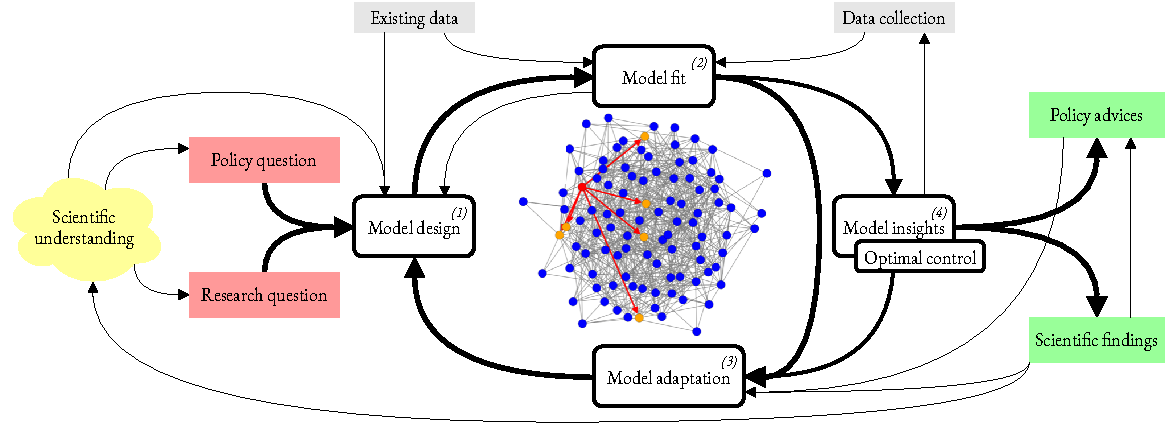
\includegraphics{fig/modeling_cycle}
  \caption[Processes for infectious disease modeling][-1\baselineskip]{Processes for  infectious disease modeling. The numerous feedback loops makes this procedure iterative. All boxes save for data collection were explored in this thesis. The central figure represents an agent-based model of disease transmission in a random graph (by Thomas Fry, a master student supervised during this thesis, with permission).}\label{fig:modeling}
\end{figure*}
\paragraph{Model fit} \textit{Fitting} conditions the model on the observed data. It allows one to infer unobserved states and parameters from reported quantities, such as the reduction of transmission during lockdown from hospitalization and deaths. A panel of methods for fitting a model to data has been developed. Usually computer-age statistical inference relies on thousands of model simulations to explore the high dimensional parameter and state spaces; each realization being evaluated against the data. The inner working of the fitting algorithms varies depending on the formal framework it is built on, but also on the numerous computational tools to make inference fast and precise. In this thesis, two classes of methods are used: Bayesian methods based on Markov chain Monte Carlo (MCMC) derivatives and frequentist Iterated Filtering (IF) methods. Fitting the model allows one to uncover previously unknown transmission parameters and unobservable states. As such, it requires a high-degree of care as inferred features may be caused by modeling artifacts instead of real epidemic features. Moreover results may misrepresent the uncertainties associated with the process and beware these methods fail more or less gracefully, thus it is possible to obtain results that seem reliable but are invariably wrong.
 
\paragraph{Model adaptation} An evaluation of the \textit{fit} of the model and the implications on the results is done by performing visuals and formal checks. More often than not, it is necessary to adapt either the fitting procedure or the model structure. It could be the inclusion or the removal of a process from the model. Or perhaps choosing to account for dynamics in a more or less explicit, detailed way. Models are lossy compressions of reality (from an information theory point of view), and choices on the processes to be included, and how to include them are the cornerstone of epidemiological modeling. Indeed despite its recent formalism, statistical inference remains an art, uncomfortably dependent on the practitioners, their backgrounds and their expectation\footnote{Multi-modeling studies -- where several modelers are tasked to answer the same question -- uncover the importance of the choices while performing statistical inference and mitigate the issues linked to opinionated model design.}. The cycle \textit{design}$\rightarrow$\textit{fit}$\rightarrow$ \textit{adapt} is then repeated until the predictive accuracy is satisfying for the goal of the exercise. 

\paragraph{Model insights}  Armed with a reliable model whose parameters and states are consistent with data and knowledge about an epidemic, it is now possible to answer the research questions. A model that reproduces observed dynamics may accurately represent epidemiological processes. It can be used as a substitute for experiments: it enables to simulate different intervention scenarios and to evaluate the impact of past or planned policies on a virtual system. This sets the range of expectations one can have with regard to the real world consequences of modeled policies. In some cases, the model is designed to replicate mechanistic relationships between the epidemiological processes, and several different models might be compared to identify which transmission routes are responsible for the observed dynamics.  Finally, the communication of model results ought to come with proper awareness of the limitations, as models are always incomplete and biased in reproducing the real epidemiological dynamics. It provides an additional opportunity for feedback towards an eventual adaptation of the model\cite{Heesterbeek:ModelingInfectiousDisease:2015}. 

\paragraph{Optimal control} Another application of epidemiological models explored in this thesis is their integration with optimal control methods to search for the \textit{best} intervention against infectious diseases. Optimal control methods are recent mathematical optimization procedures extending the calculus of variations to enable the derivation of control policies for dynamical systems. While technical adaptations are necessary to perform optimal control on epidemiological models, this rigorous framework identifies the most effective control measures under a set of operational constraints, discovering non-intuitive features and policies. These optimal interventions exploit every features of the complex interactions modeled, allowing to \eg best allocate a limited vaccine supply in space and time. Such tools, currently in their infancy and requiring accurate models, are promising as reasoning aid, uncovering another facet of disease transmission, and for the effective allocation of control resources in the fight against epidemics.



%\sidenote[][8\baselineskip]{Multimodeling studies and collaborative experiments strive to mitigate this issue by bringing together assumption and projections by different groups. See \eg \url{covid19forecasthub.org/community}}.

\section{Thesis aim and outline}
\begin{table*}[t]
\label{tab:allmodels}
\centering\small
\begin{tabularx}{\textwidth}{x{14mm}cccx{15mm}cx{15mm}p{30mm}}
\toprule
   \small{\textsc{Chapter}}     & Disease           & Compartments & Processes         & \small{$N_{\text{spatial}}$} & Fit       & Aim            & Reference\\
\midrule
4 & Cholera           & SEIR+B      & Stochastic    & --           & IF-like  & explain         & \tiny{\fullcite{Lemaitre:RainfallDriverEpidemic:2019}}\\
4 & Cholera           & SEIR+B      & Deterministic & --             & MCMC-like & explain        & \tiny{\fullcite{Lemaitre:RainfallDriverEpidemic:2019}}\\
5  & Cholera           & SEAIR$^3$+V & Stochastic    & 10        & IF-like   & project (scenarios)       & \tiny{\fullcite{Lee:AchievingCoordinatedNational:2020}} \\ \addlinespace
6  & \textsc{\textsc{covid}}-19 & SEI$^3$R+VH & Stochastic    & 3’000+    & MCMC-like & project (scenarios)        & \tiny{\fullcite{Lemaitre:ScenarioModelingPipeline:2021}} \\
7  & \textsc{\textsc{covid}}-19  & SEI$^3$R+H  & Stochastic    & --             & IF-like  & infer           & \tiny{\fullcite{Lemaitre:AssessingImpactNonpharmaceutical:2020}}\\
8  & \textsc{\textsc{covid}}-19  & SEIAR+VH    & Deterministic & 107       & MCMC-like & optimal\newline control & \tiny{\fullcite{Lemaitre:OptimizingSpatiotemporalAllocation:2021}}\\ 
\bottomrule
\end{tabularx}
\caption[Summary of the models described in this thesis]{Summary of the compartmental models described in this thesis.}
\end{table*}
The present thesis has been developed within the Swiss National Foundation project ``Optimal control of intervention strategies for waterborne disease epidemics (\textsc{snf} 200021–172578)’’. It initial goal was to develop a decision support system for the real-time design of optimal intervention strategies against cholera, which includes an operational forecasting tool coupled with an optimal control solver. This framework has been developed, albeit for \textsc{covid}-19 transmission in Italy, and is presented in \textsc{Chapter~6}. 


The work presented extensively builds on the ECHO laboratory expertise on the spatially-explicit modeling of cholera transmission\footnote[][2\baselineskip]{and waterborne diseases in general; see: \fullcite{Rinaldo:RiverNetworksEcological:2020a, Rinaldo:Reassessment20102011:2012}}. The group has developed over a decade a rainfall-mediated, spatially explicit cholera model that has inspired each of the other models presented in this thesis. The original model is presented in \textsc{Chapter~1} with a short introduction on the ancient disease that is cholera, and its sorrowful history.

Cholera is the focus of two additional chapters. The explanatory power of two existing models linking cholera transmission with rainfall are compared in \textsc{Chapter~2}, through the analysis of an outbreak in Juba, South-Sudan. In \textsc{Chapter~3}, a scenario planning estimation of the probability of eliminating cholera from Haiti through a mass vaccination campaign is presented; this work has been carried within the framework of a multi-modeling study with other groups, and input from the ministry of health of Haiti.
%\marginnote[-5\baselineskip]{Most bibliographic items and some additional precision are presented as margin notes for convenience. However, the full bibliography is included at the end of the thesis.}

The remaining chapters focus on \textsc{covid}-19. In \textsc{Chapter~4}, some facets of dealing with uncertainties from an emerging disease pandemic are uncovered, with a focus on a pipeline for scenario modeling that has been used to inform governments, in the United States and in other countries. 
Using data collected while participating in the \textsc{covid}-19 response, it was possible to estimate the impact of early interventions against \textsc{covid}-19 in Switzerland, this study is presented in \textsc{Chapter~5}. %\marginnote[-5\baselineskip]{Incidentaly, this organisation reflects the chronogical order of the work.}
And finally, \textsc{Chapter~6} presents how to integrate a spatially explicit epidemiological model for the Italian epidemic within an optimal control framework in order to discover the optimal strategy for vaccine allocation.





%%
% Start the main matter (normal chapters)
\mainmatter

\part{Cholera modeling}
\begin{fullwidth}
\chapter{A modelling oriented primer on cholera}
\end{fullwidth}
Cholera is an acute intestinal infection causing severe diarrhea that may lead to dehydration, and sometimes death. While the global burden of cholera is difficult to estimate as the majority of cases are not reported, it is estimated that 3 million cases and 95'000 deaths occurs every year in endemic areas (around 50 countries), with millions more at risk\cite{Ali:UpdatedGlobalBurden:2015}. Despite its household name, cholera belongs to the neglected tropical diseases group as our understanding of many important aspects of cholera clinical course and transmission is limited.
A political will to eliminate this ancient disease has recently arisen. The World Health Organization (WHO) initiated the Global Task Force for Cholera Control (GTFCC), who provides a concrete path towards the elimination of cholera by 2030\footnote{Elimination being defined as a 90\% reduction of cholera deaths/year, see \url{gtfcc.org} for more information.}. The general consensus is that to reach this goal in endemic countries, there must be substantial long-term improvements in safe water distribution systems, adequate sanitation and accessible hygiene education.  Moreover, in the event of a cholera outbreak, timely interventions such as vaccination campaigns are crucial to limit the spread of the disease, and proper medical treatment reduce the toll of the disease on communities. %With limited resources, public health officials face a number of challenging decisions, and a data driven decision support to guide the rational deployment of cholera control strategies is needed. Furthermore, on the road toward elimination, the need to setup context-specific tailored approaches appears. 
%The poorest of the poor
%most infected individuals are asymptomatic, i.e., they do not present symptoms, while other experience mild or severe symptoms.  %Since their mobility is not hindered, they become a vector of the infection. If not properly treated, cholera can kill children and adults within hours. 


\vspace{.7cm}
\section{History and epidemiology}
\begin{marginfigure}%[0\baselineskip]
%\centering
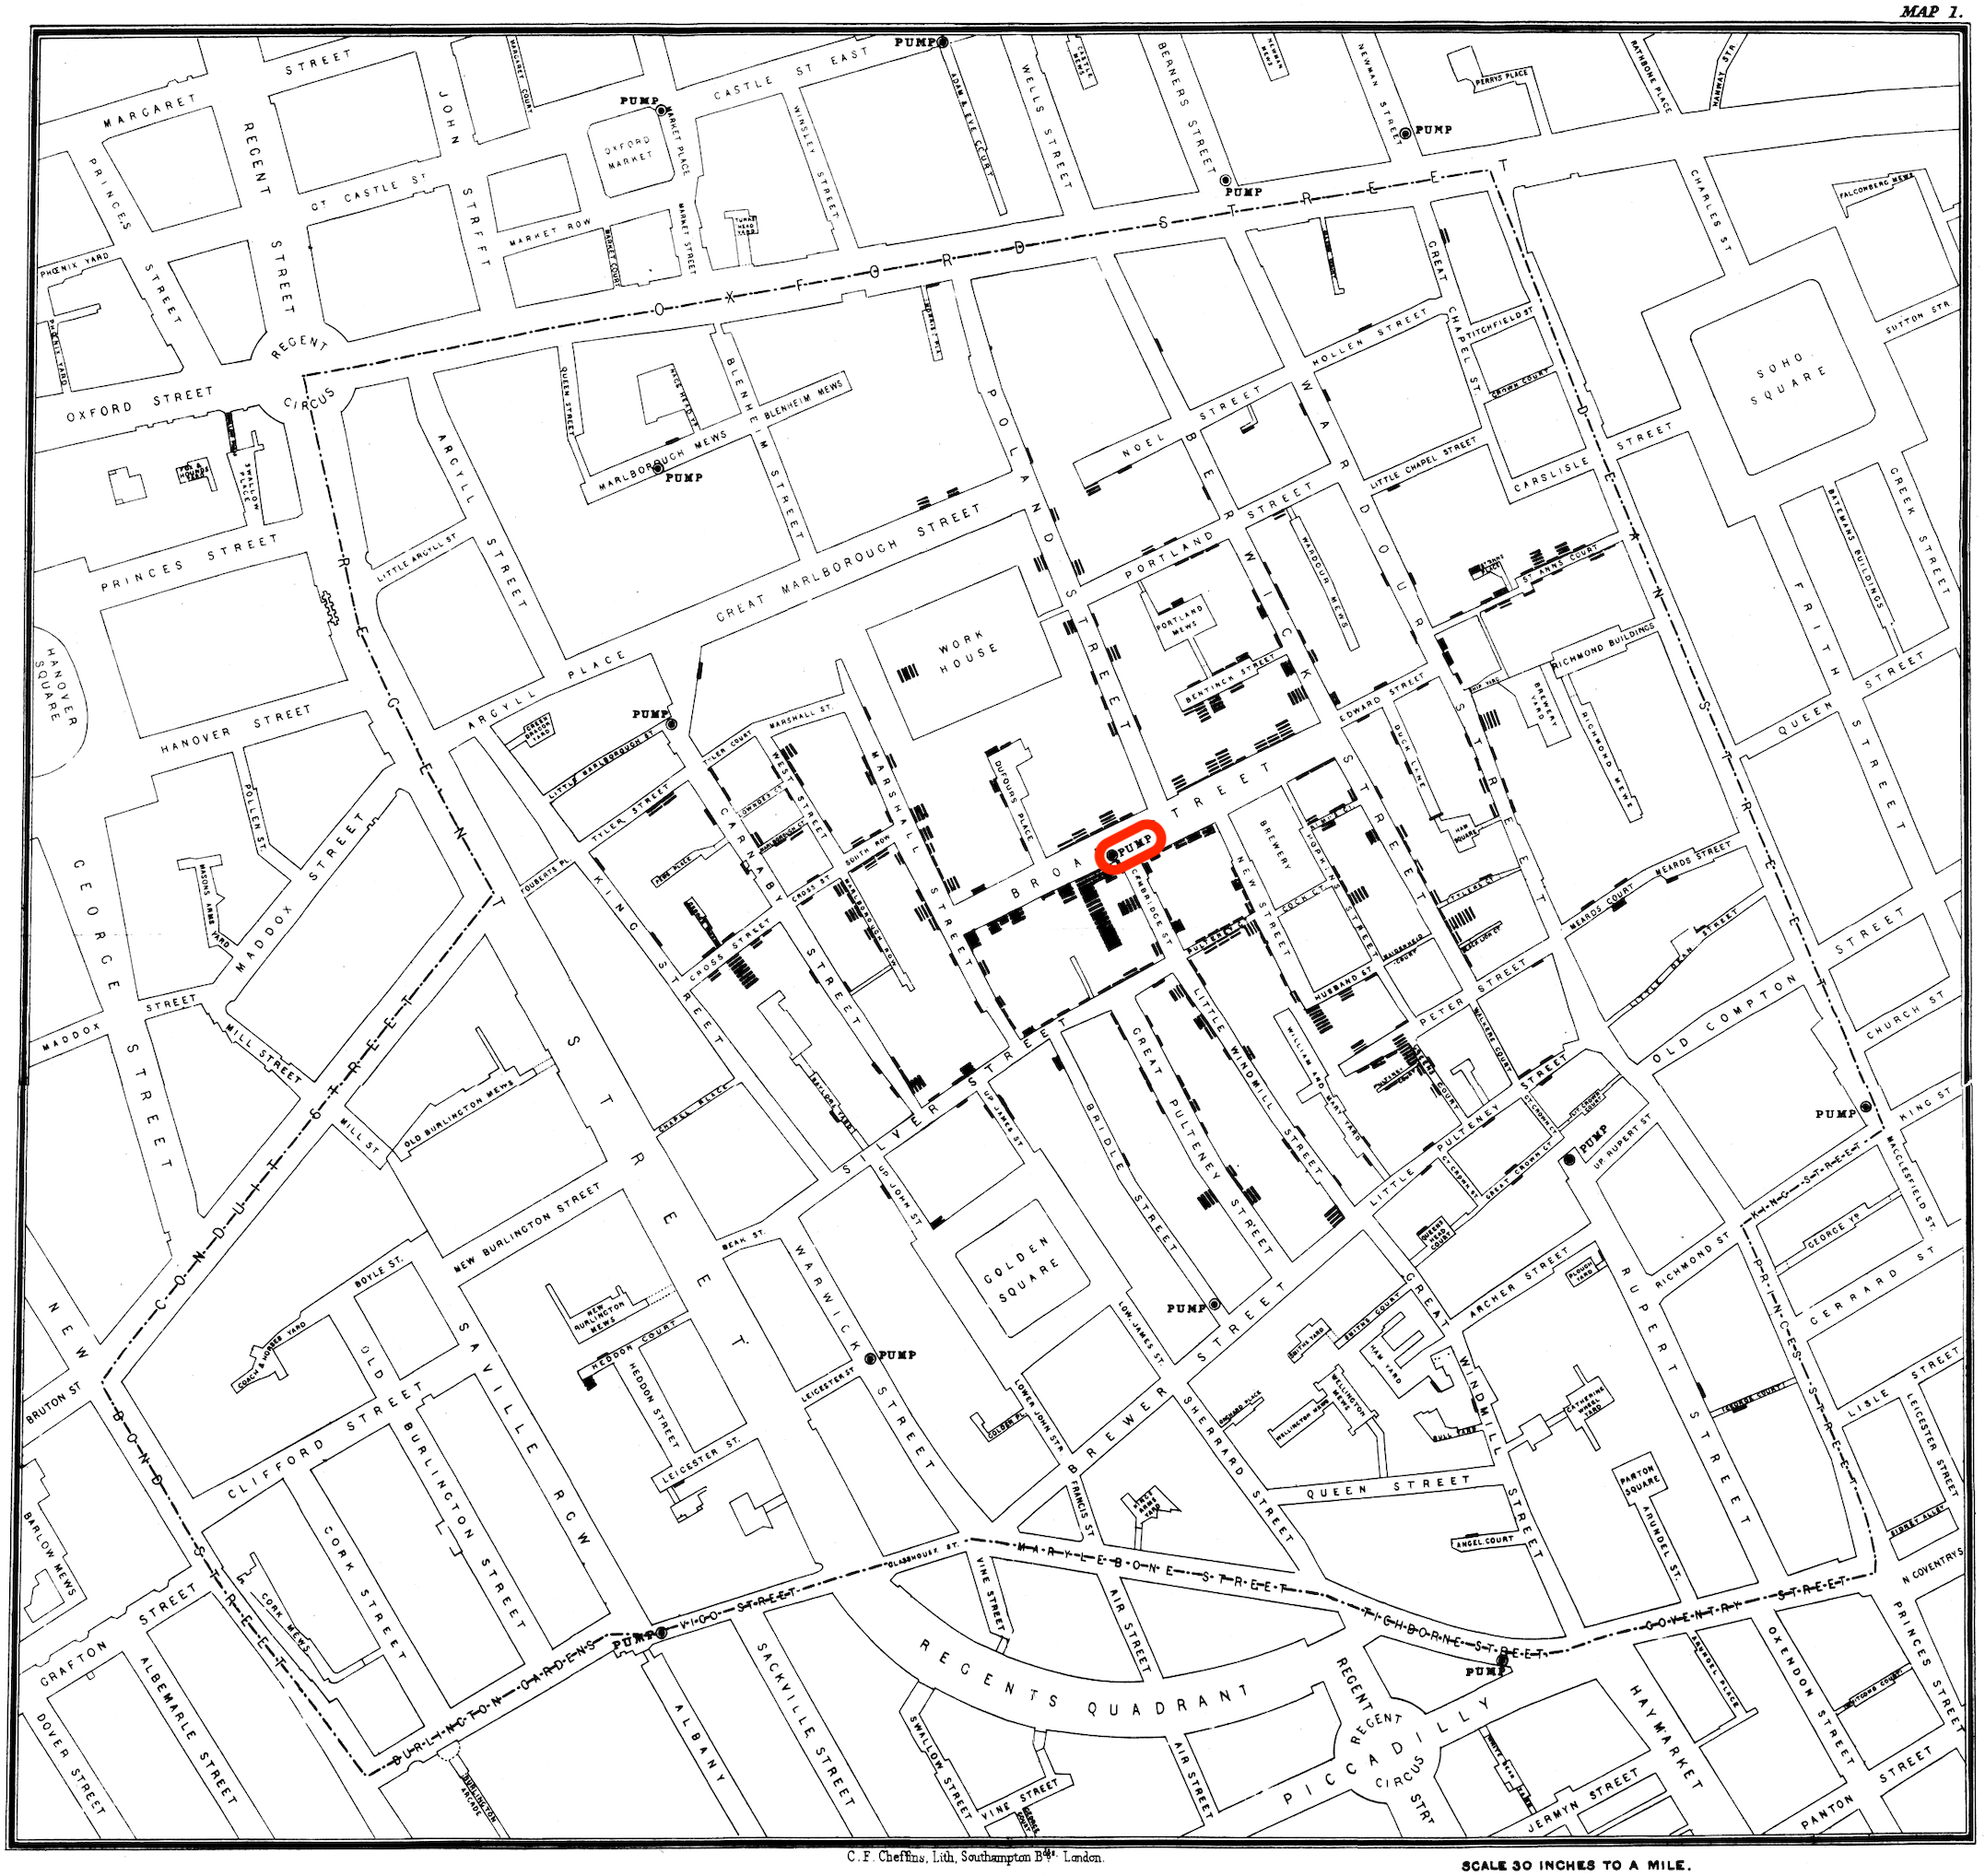
\includegraphics[width=\textwidth]{fig/snow-cholera-map_edit}
\margincaption[John Snow map of cluster cholera cases in London, 1854]{Original map by John Snow. Stacked rectangles represent cholera cases of the 1854 Broad Street outbreak. The work of John Snow conviced the authorities to close the water pump (circled in red), leading to a decrease in Mortality. Lithography by Charles Cheffins, in "\fullcite[p. 54]{Snow:ModeCommunicationCholera:1855}.}\label{johnsnow}
\end{marginfigure}
Humanity and cholera share a long history, with supposed mentions as early the 5th centurey \textsc{bce}. The disease became more widely know in the modern era. From 1817 to 1923, six successive pandemics -- all originated in the delta of the Ganges river, but taking different paths accross the world -- occured. Cholera spread around the world owning to the the nascent mobility, leaving 10s of millions dead accross countries and continents.  Scientific developments sped up during the third cholera pandemic (1846-60). In 1854, a cholera outbreak in Broad Street (Soho, London) was studied by physician John Snow and lead to an impressive early work in investigative epidemiology and public health. Analyzing the contamination pattern among residents, Snow postulated that cholera spread through water contaminated by an infectious agent, instead of foul air\sidenote[][-1\baselineskip]{At the time, the accepted mode of contamination for cholera and many other disease was through miasma, \textit{bad air} contaminated by organic matter. Chasing odor  justified urban amangement along streets and river banks in Paris and London. But also in Lausanne, where rivers Flon and Louve where covered in 1832 in response to a cholera outbreak. The cholera dish from Valais is a testimony of the strong impression cholera left on the Swiss.}.  Simultaneously, Italian microbiologist Filippo Pacini isolated the bacterium in Florence. Thirty years after Pacini, German scientist Robert Koch independently rediscovered the cholera pathogens after investigation in Egypt and India and first posited its causative relationship with the disease. Finally a hundred year later, Indian researcher Sambhu Nath De discovered the cholera toxin in 1959.

Throughout the seventh pandemic from 1961 onwards, cholera spread in several waves, through Asia in the 1960s, reachin Africa and the Middle East in the 1970s and the Americas in 1991\cite{Mutreja:EvidenceSeveralWaves:2011}. Improvement in sanitation and hygiene spared higher income country from disease, and cholera became a burden of the poorest of the Global South. Series of outbreaks (\eg Zimbabwe 2008, Haïti 2010, Yemen 2016), continuous transmission in endemic countries and millions at risks keeps this ancient disease a ongoing public health issue.

The span of this thesis was marked by a cholera outbreak in Yemen (2016--2021) -- an humanitarian crisis with 2.5M suspected cases and nearly 4'000 deaths -- an outbreak in Zimbabwe and flare up in Algeria in addition to seasonal outbreaks and endemic cholera transmission in the Asia and sub-saharian Africa.  But also by the last confirmed cases of cholera in Haiti in 2019.

While the number of cholera cases doubled from 2018 to 2019 to nearly a million, reported cholera death decreased to less than 2'000 in 2019, with Africa reporting lowest number since the 2000s. Haiti reported its last confirmed cholera cases in january 2019, bringing hope to cholera elimination from its last foothold in the Americas. Effort towards improvement of sanitary conditions and reactive vaccinations (24M doses of cholera vaccines were distribued in 2019) hope to bring these number down\footnote{see \fullcite{WHO:Cholera2019:2020} and previous \textit{Weekly Epidemiological Records} about cholera.}. 

In the following we highlight some relevant aspects about cholera transmission, while leaving some biological and medical features of cholera outside the scope of this thesis.


\section{Pathogen} 
\begin{marginfigure}[6\baselineskip]
\centering
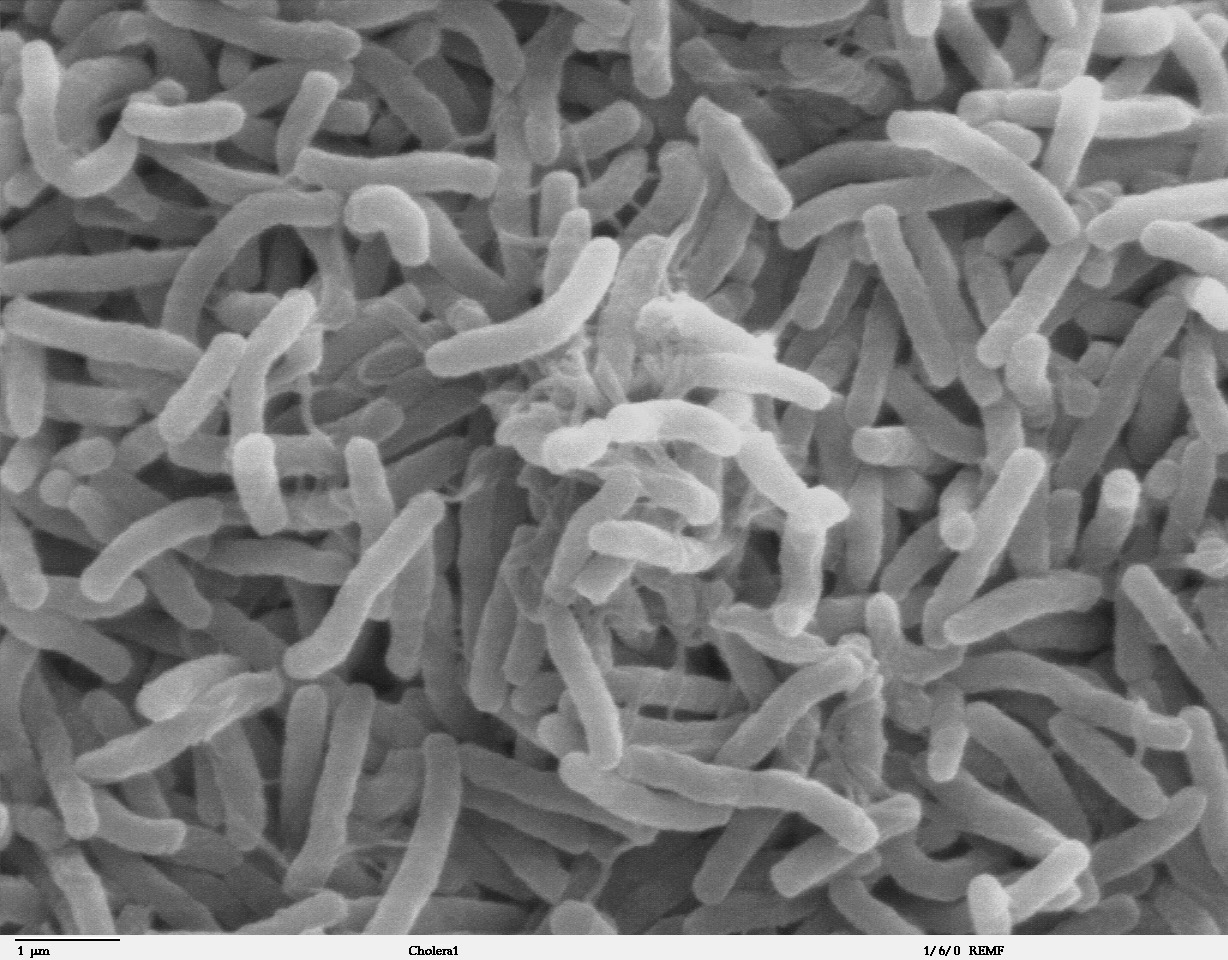
\includegraphics{fig/vibrio}
\margincaption[Vibrio cholerae bacteria]{Scanning electron microscope image of \textit{Vibrio cholerae} (Public domain image by Ronald Taylor, Tom Kirn, Louisa Howard).}
\label{rain}
\end{marginfigure}
\paragraph{Pathogen} Cholera is an infection caused by a waterborne bacteria: the \emph{Vibrio cholerae}. While many serogoups of \emph{V. cholerae} can secrete the cholera toxin reponsible for massive watery diarrhea, only serogoups O139 and O1 are responsible for disease epidemics. O1 is causing most recent epidemics, and is divided in two biotypes: Classical O1 and El Tor, which are both divided into three serotypes: Ogawa, Inaba and the rare Hikojima\cite{Kaper:Cholera:1995}. Cholera classification has its importance as it affects many epidemiological characteristic \eg, El Tor survives longer in water and has an higher asymtomatic/symptomatic ratio\cite{WHO:CholeraVaccinesWHO:2017}. The current cholera pandemic is mainly caused by El Tor, while the Classical derivative caused previous fifth and sixth pandemic and is now limited to the Gange delta\cite{Nair:CholeraDueAltered:2006}. 

 \paragraph{Environmental reservoir}  \textit{V. cholerae} exists as natural habitant in some aquatic ecosystem, in particular in brackish waters and estuaries. There is no marine host, but complex ecological association processes take place in the aquatic medium, and natural genetic transformation is enabled by chitin, the polymer constituting the crustacean exoskeleton\cite{Reidl:VibrioCholeraeCholera:2002,Meibom:ChitinInducesNatural:2005}. There is no concensus on how long \textit{V. cholerae} remains infectious in water and under which conditions it is able to reproduce\cite{Mavian:ToxigenicVibrioCholerae:2020}. In cholera epidemics, it is difficult to isolate the role of the natural cholera reservoir from freshly introduced \textit{Vibrios} from the feces of an infected person, though the later is suspected to drive  transmission during outbreaks.

\paragraph{Climatic Drivers} Cholera expresses marked seasonality patterns that takes different shapes in accross setups. A complex and unclear association between precipitation and cholera infections has been put forward in many research works. After hurricane Matthew and heavy rainfall in October 2016, a cholera flare-up started from low transmission in Haiti\cite{Pasetto:RealtimeForecastingCholera:2018}. Similarly, cholera in many African countries follows a seasonal trend, with the epidemiological curve raising during the rainy season\cite{Baracchini:SeasonalityCholeraDynamics:2017}.  Rainfalls might play a major role in water contamination, for instance through the washout of open-air defecation and raw sewage circulation in the environment. A litterature review of the relationship between cholera and rainfall is provided in the next chapter. Temperature, water acidity, sunlight and other environemental factors have also been shown to affect the survival and reproduction of \textit{V. cholerae} in water bodies. Hence macro climate phenomena such the El Niño Southern Oscillation have been associated with changes in transmission, even if no causal link could be established\cite[-2\baselineskip]{Pascual:CholeraDynamicsNinoSouthern:2000}\footnote{Marc Lipsitch and Cécile Viboud beautifully describe the difficulty evaluating the environmental factors in disease transmission, writing for influenza: "This potpourri of possible mechanisms places us in a kind of Popperian purgatory, in which data in support of every hypothesis exist, yet none of the hypotheses has been subjected to tests that are rigorous enough to reject it." in \fullcite{Lipsitch:InfluenzaSeasonalityLifting:2009}}.

\section{Cholera in the human} 
\paragraph{Disease} An human host becomes infected through the ingestion of a critical dose of \emph{V. cholerae}\shortcite{Kaper:Cholera:1995,Nelson:CholeraTransmissionHost:2009}. The susceptibility depends on many factors such as gastric acidity and age, with under 5 much more likely to become infected\cite{Sack:Cholera:2004}. \textit{V. cholerae} colonize the small intestine for an incubation period lasting 12 hours to 5 days\cite{Azman:IncubationPeriodCholera:2013} before symptoms. Then, a wide range of outcomes are possible. Most of the time the infection is inapparent, resulting in asymptomatic individuals. On the other end of the spectrum severe infection (or \emph{cholera gravis}), caracterized by vomiting and profuse rice water diarrhea, occurs in 1\% to 15\% of the cases. Many stages of mild infections lie between asymptomatics and severe infections. Unless tested in a laboratory, symptoms are indistinguishable  from those of numerous other infections causing diarrhea\footnote{\fullcite{King:InapparentInfectionsCholera:2008};  \fullciteshortb{Kaper:Cholera:1995, Nelson:CholeraTransmissionHost:2009}; \fullcite{vandeLinde:ObservationsSpreadCholera:1965,Mccormack:CommunityStudyInapparent:1969}}.  The severity of illness correlates with the quantity of \textit{V. cholerae} ingested\cite{Brouwer:DoseresponseRelationshipsEnvironmentally:2017}, and depends on the cholera strain and personal characteristics, immunity, pregnancy, blood type\cite{WHO:CholeraVaccinesWHO:2017,Azman:IncubationPeriodCholera:2013}, ...%Table 1 for a review of individual data studies.
Treatment is crucial: severely infected individuals migth loose up to 20 litres of water through diarrhea a day and may die within hours. If left untreated, natural mortality reaches up to 60\% but proper therapy lowers mortality below 1\%\cite{Luquero:MortalityRatesCholera:2016}.

\paragraph{Shedding and transmission} The intensity of the bacterial shedding varies with the intensity of the infection. It is estimated to range from $10^3$ to $10^{9}$ vibrios per gram of stool for asymptomatic infected and severely infected individual respectively\shortcite{Nelson:CholeraTransmissionHost:2009}. Similarly, the duration of the shedding period typically ranges from a day up to two weeks\shortcite{Nelson:CholeraTransmissionHost:2009, Kaper:Cholera:1995}.
Transmission occurs along the fecal-oral route (consumption of contaminated water or food, contact with fomites), but contamination is also possible from aquatic reservoirs, through water or seafood. Freshly shed \textit{Vibrios} may be in an hyperinfectious state, which could be of great importance in driving epidemic transmission\cite{Butler:CholeraStoolBacteria:2006}. The principle mechanism of transmission is the intake of water contaminated by the untreated diarrheal discharge of other infectious individuals.
Asymptomatic individuals remains mobile and shed bacteria, thus may be of importance for cholera dissemination.

\paragraph{Human mobility and hydrological transport} Spatial spread of cholera outbreaks may occurs through two networks. \textit{V. Cholerae} may be transported through the river network. A example is the spread of the 2010 Haiti epidemic along the Artibonite river\cite{Piarroux:UnderstandingCholeraEpidemic:2011}. Human mobility also plays a major role in the spreading of the infections possibly due to the large number of asymptomatic that transport and disperse cholera across a country or even worldwide.  Indeed also in Haiti, cholera was brought into Haiti by infected United Nations peacekeepers\cite{Piarroux:UnderstandingCholeraEpidemic:2011}. %However, mobility, especially in humanitarian crisis situations often associated with cholera, remains difficult to predict\cite{Lu:PredictabilityPopulationDisplacement:2012,Riley:LargeScaleSpatialTransmissionModels:2007,Bengtsson:ImprovedResponseDisasters:2011,Rebaudet:DrySeasonHaiti:2013}.

\paragraph{Immunity} Infected individuals that recover from the infection are immunized against \textit{V. cholerae}  of the same serogroup. The duration of acquired immunity is difficult to estimate, and depends on many factors. Acquired immunity has been reported to range from few months to several years \footnote{Most current estimages ranges from 2 to 10 years.}, possibly depending on the virulence of the infection\cite{Levine:DurationInfectionDerivedImmunity:1981,Kaper:Cholera:1995,Woodward:CholeraReinfectionMan:1971,Glass:SeroepidemiologicalStudiesEI:1985,Clemens:BiotypeDeterminantNatural:1991,Leung:ProtectionAffordedPrevious:2021}.

\subsection{Cholera Control} 
Cholera interventions may be preventive or concern the treatment of infected individual. Treatment plays an important role in reducing the reproduction number of the epidemic and mainly consists of:
\begin{description}
\item[Oral (or Intravenous) Rehydratation Therapy] The main treatement for cholera consists of replacing fluids as fast as they are lost. Despite its simplicity, it is very effective in reducing mortality. Fluids with the same electrolyte composition must be administred\cite{Kuhn:GlucoseNotRiceBased:2014}.  Rehydratation is usually done in treatment centers, but may take place at the patient home. This differentiation might determine if stools contribute to the infection cycle or are properly disposed.
\item[Antibiotics] reduce the severity and the duration of the infection. WHO recommends their use only for the most severe cases as antibiotic resistance of \emph{V. cholerae} is raising worldwide\cite{Sack:GettingSeriousCholera:2006}.
\end{description}

Prevention measures may be carried out before and during the outbreak, and are described below.

\paragraph{Surveillance \& Reporting} During an outbreak, surveillance consists of the timely reporting of new cases. In many countries where outbreaks occurs annually during the rainy season, the observation of past epidemics provides insight on the severity and timing of the infection that can be used for preparation\cite{Baracchini:SeasonalityCholeraDynamics:2017}. Environmental surveillance, monitoring for \textit{V. Cholerae} in the water, is also possible. However, never has \textit{V. Cholerae} been found in the environment before an epidemic. 
Without laboratory equipement, it is impossible to distinguish cholera from another pathogen in a patient with acute watery diarrhea. The has been an effort to standardize the clinical definition of a suspected cholera case, which varies between countries and during outbreaks. A suspected case combine acute watery diarrhea and severe dehydration, the latter condition being dropped in case of outreak. This diagnosis can be validated using rapid diagnosis tests (RTDs), with a pretty high sensibility but low sensitivity. Precise indentification is obtained through culture, the current gold standard\footnote{\fullcite{Camacho:CholeraEpidemicYemen:2018} and \fullcite{CDC:DiagnosisDetectionCholera:2018}}. RTDs and culture are not always available, especially during an outbreak.  As a consequence, over-reporting during an outbreak situation is likely, as is under reporting as transmission settings might be isolated or plagued with conflicts, natural disaster. WHO guidelines recommend that, when a patient enters a treatment center, his name, address, sex, age (over or below 5) and symptoms are recorded\cite{WHO:FirstStepsManaging:2010}. % https://apps.who.int/iris/bitstream/handle/10665/334241/WER9537-eng-fre.pdf?ua=1 end, and https://www.cdc.gov/cholera/diagnosis.html

\paragraph{WaSH} Water, Sanitation and Hygiene (WaSH) is a broad term that includes many intervention strategies that are key to the long term elimination of cholera. The improved sanitary conditions have been the main factor that led to cholera elimination  in first world countries. WaSH is divided into short and long term measures. Short term strategies involve sterilization, decontamination, hand washing, education sessions and water purification and filtering (chlorination, ...)\cite{Rebaudet:NationalAlertresponseStrategy:2018,Fewtrell:WaterSanitationHygiene:2005}. Long-term sanitation strategies involve the construction of infrastructures for fecal sludge management, sewage systems, toilets and access to safe water sources. From a modeling point of view, WaSH reduces exposure (water purification, sari filtration) and shedding (sewage and fecal sludge management). By its nature and its delayed, longterm effects, WaSH improvement is difficult to quantify in modeling framework.

\paragraph{Vaccination} is a safe and effective way to protect individuals from cholera, and to reduce the propagation of the epidemic. It can be used in a preventive or reactive way. Several vaccine exists for cholera, with different characteristics. As of today, two main oral cholera vaccines (OCVs) are used in vaccination campaigns around the world: WC-rBS and BivWC\footnote[][-3\baselineskip]{An other vaccine, Vaxchora, was recently approved by the FDA, mostly for travelers.}. The main characteristics of these two vaccines are shown in Table~\ref{tab:vacc}.

\begin{table}[h]
\centering\small
\label{tab:prior}
\begin{tabular}{lp{40mm}p{40mm}}
\toprule
Generic Name &  BiWC & WC-rBS\\ 
\midrule
Commercial name   &  mORCVAX, Shanchol,  Euvichol, Cholvax & Dukoral  \\
Target strain O1 &   yes (classical, El Tor, Ogawa, Inaba)& yes (classical, El Tor, Ogawa, Inaba), also  target a cholera toxin  \\
Target strain O139   &  yes &      no     \\
Doses   &  2 doses, 2 weeks apart & 2 doses (3 for children) 1--6 weeks apart  \\
%Vaccine Efficacy & 58\% &  \\
Field Effectiveness  & between 37\% and 87\% for two years & 78\% protection 1--6 months after vaccination\\
Age   &  $>$ 1 year & $>$ 2 year      \\
Usage & Mass vaccination, Global OCV stockpile, 25M doses administered & Mainly for travelers ($>$ 1M doses administered)\\
Protection length & 3 years (1 dose: short term protection) & 2 years\\
Constraints & -- & needs buffer solution\\
Price per dose & 1.85\$ & 5.25\$ \\ 
Usage & Since 1998 in most recent outbreaks & Between 1997 and 2009 in Uganda, Tanzania, Indonesia,~... \\
\bottomrule
\end{tabular}
\caption[Characteristic of currently available vaccines][-2\baselineskip]{Characteristic of currently available vaccines. The proposed value for field effectiveness, along with vaccine efficacy (not shown here) is really difficult to evaluate, cannot be written in a simple way without omitting crucial information. A good review of research on cholera vaccine is the WHO Position paper on cholera vaccines~\fullcite{WHO:CholeraVaccinesWHO:2017}. See also~\textcite{WHO:BackgroundPaperWholeCell:2017,Azman:PopulationLevelEffectCholera:2016,Luquero:FirstOutbreakResponse:2013,WHO:BackgroundPaperIntegration:2009,Luquero:UseVibrioCholerae:2014,Qadri:EfficacySingledoseRegimen:2018,Bi:ProtectionCholeraKilled:2017,Azman:ImpactOneDoseTwoDose:2015,Tohme:OralCholeraVaccine:2015}.}
\label{tab:vacc}
\end{table}

 Vaccine can either be administered in a targeted fashion or to whole populations in mass vaccination campaigns. Despite effort to build a worldwide vaccine stockpile, demand for cholera vaccine vastly exceeds supply\cite[-1\baselineskip]{Parker:AdaptingGlobalShortage:2017a,Seidlein:PreventingCholeraOutbreaks:2018}.


\section{Cholera Modeling}
Cholera modeling has received renewed a lot of attention during the 2010 Haiti outbreak, and serves different purposes. 
Most of recent modeling efforts focus on phenomenological (or statistical) models with different degrees of deterministic processes\shortcite[-2\baselineskip]{Azman:UrbanCholeraTransmission:2012,Finger:PotentialImpactCasearea:2018,Camacho:CholeraEpidemicYemen:2018,Lessler:MappingBurdenCholera:2018,Koelle:DisentanglingExtrinsicIntrinsic:2004}. Mechanistic cholera models embed uncertainties into their parameter distribution, and differ in the way they account for the epidemiological processes\shortcite{Kirpich:ControllingCholeraOuest:2017,Tuite:CholeraEpidemicHaiti:2011,Chao:VaccinationStrategiesEpidemic:2011,Kirpich:CholeraTransmissionOuest:2015}. Most cholera models are spatially implicit, however there have been a number of attempts to describe the spatial spread of the epidemic. For example, Andrew and Basu used an approach with isolated nodes and independent transmission parameters in each node\shortcite{Andrews:TransmissionDynamicsControl:2011}.

\subsection{ECHO's cholera model}
A spatially-explicit model has been developed at ECHO in the past 10 years \parencite{Bertuzzo:SpacetimeEvolutionCholera:2008}. It has been used for studies on the dynamics of several cholera epidemics, such as in South Africa in 2000 \parencite{Mari:ModellingCholeraEpidemics:2012}, Senegal in 2005, Haiti from 2010 to 2019 \parencite{Bertuzzo:PredictionSpatialEvolution:2011,Bertuzzo:ProbabilityExtinctionHaiti:2016}, Democratic Republic of the Congo from 2004 to 2011 and many others\cite{Finger:PotentialImpactCasearea:2018}.  
We present here a complete formulation of the model, including patterns and effectiveness of vaccinations, human and hydrological mobility \parencite{Bertuzzo:ProbabilityExtinctionHaiti:2016,Pasetto:RealtimeForecastingCholera:2018}. This model has inspired to a various degree all the other model described in this thesis.

The model is a variation of the SIR model introduced first by Kermack and McKendrick\cite{Kermack:ContributionMathematicalTheory:1927}, with additional compartments for the vaccinated individuals and the bacteria concentration in the environment.

The model subdivides the area potentially concerned by the epidemic into $n$ sub-regions. The sub-regions, defined by political boundaries or geomorphological features (like watersheds\cite{Bertuzzo:ProbabilityExtinctionHaiti:2016}), are represented as connected nodes. The $n$ nodes represent $n$ human communities having population size $H_i$, $i=1,\dots, n$. 

At time $t$ and for each node $i$, the individuals in the node can be grouped into six compartments:

\begin{itemize}
\item $S_i(t)$: susceptible individuals  have no immunity, and may enter in contact with the bacteria and become infected (symptomatic or not),
\item $I_i(t)$: infected individual shed bacteria into the community reservoir,
\item $R_i(t)$: recovered are temporally immune, and don't participate in disease transmission,
\item $V^S_i(t)$: vaccinated susceptible,
\item $V^I_i(t)$: vaccinated infected,
\item $V^R_i(t)$: vaccinated recovered.
\end{itemize}

In addition, the model considers the bacterial concentration of \textit{V.~cholerae} in the water reservoir of the community, $B_i(t)$. The $n$ nodes are connected by both human mobility and pathogen transport through water.

Individuals commute from node $i$ to node $j$ with probability $Q_{ij}$. Bacteria are transported along the river network from node $i$ to node $j$ with probability $P_{ij}$.

The cholera dynamics are described by the following set of coupled ordinary differential equations:
\begin{fullwidth}

\begingroup
\allowdisplaybreaks
\begin{eqnarray}
\frac{dI_i}{dt} &=& \sigma F_i(t) S_i - (\gamma + \mu + \alpha) I_i \label{eq:I2}\\
\frac{dR_i}{dt} &=& (1-\sigma) F_i(t) S_i + \gamma I_i - (\rho + \mu+\frac{\nu_i(t)}{S_i+R_i}) R_i \label{eq:R2}\\
\frac{dV^S_i}{dt} &=& \nu_i(t) \frac{S_i}{S_i+R_i}-\mu V^S_i \label{eq:VS2}\\
\frac{dV^I_i}{dt} &=& \sigma (1-\eta) F_i(t) V^S_i - (\gamma + \mu + \alpha) V^I_i \label{eq:VI2}\\
\frac{dV^R_i}{dt} &=& \nu_i(t) \frac{R_i}{S_i+R_i} + (1-\sigma) (1-\eta) F_i(t) V^S_i + \gamma V^I_i - (\mu+\rho_v) V^R_i \label{eq:VR2}\\
\frac{dB_i}{dt} &=& - \mu_B B_i +\frac{p}{W_i}\left[1 + \phi J_i(t) \right] \left((1-m)(I_i +V_i^I)+m \sum_{j=1}^n Q_{ij} (I_j +V_j^I)\right)-  l \left( B_i - \sum_{j=1}^n P_{ji} \frac{W_j}{W_i} B_j \right)
\end{eqnarray}
\endgroup
\end{fullwidth}
where the population~$H_i$ of each node is assumed to be at demographic equilibrium, thus $S_i=H_i-I_i-R_i-V_i^S-V_i^I-V_i^R$.

The force of infection, i.e the rate at which individual enters in contact with the diseases, is written as:

\begin{equation}
F_i(t) = \beta \left[ (1 - m) \frac{B_i}{K + B_i} + m \sum_{j=1}^n Q_{ij} \frac{B_j}{K + B_j} \right].
\label{force}
\end{equation}

The parameter~$\beta$ represents the maximum exposure rate, which may decrease in time due to awareness of the population on the cholera transmission factors\cite{Bertuzzo:ProbabilityExtinctionHaiti:2016}. The fraction $B_{i}/(K+B_{i})$ is the probability of becoming infected due to the exposure to a concentration~$B_i$ of \textit{V.~cholerae}, $K$ being the half-saturation constant\cite{Codeco:EndemicEpidemicDynamics:2001}. The force of infection in a given node depends for a fraction ($1-m$) to the local concentration of \textit{V.~cholerae}, $B_i$, while the remaining fraction $m$, represents the community-level probability that individuals travel outside their node, accounts for the contribution of the concentration~$B_j$ of the remote communities. 
The human mobility is accounted with the matrix $Q_{ij}$ representing the probabilities that an individual living in node $i$ reaches~$j$ as a destination. Because of human mobility, a susceptible individual residing at node $i$ can be exposed to pathogens in the destination community $j$. 
In the lack of detailed mobility data,  the probabilities~$Q_{ij}$ can be estimated through a gravity approach\cite{Erlander:GravityModelTransportation:1990} to model human mobility:

\begin{equation}
Q_{ij} = \frac{H_j e^{-d_{ij}/D}}{\sum_{k \neq i}^n H_k e^{-d_{ik}/D}} \, ,
\label{eq:mob}
\end{equation}
where the attractiveness of node~$j$ depends on its population size $H_j$, while the deterrence factor is assumed to be dependent on the distance~$d_{ij}$ between the two communities via an exponential kernel (with shape factor~$D$).  

Due to the contact with contaminated water, a fraction $\sigma$ of the infected individuals develops symptoms, passing from compartment $S$ to $I$. The remaining fraction~$(1-\sigma)$ does not develop symptoms, does not contribute to the disease transmission, and is considered temporally immune, thus passing from compartment $S$ to $R$.  Symptomatic infected individuals recover at a rate~$\gamma$, or die due to cholera or other causes at rates~$\alpha$ or $\mu$, respectively.
Recovered individuals lose their immunity at rate~$\rho$, thus passing from compartments $R$ to $S$, or die at a rate~$\mu$.  % TODO Too many times property.

The environmental concentration of \textit{V.~cholerae} at a node $i$ may increase due to both human mobility and to hydrologic dispersion. Human contributions depends from a fraction $1-m$ on the local infected individuals and form a fraction $m$ on the symptomatic infected individuals moving according to the mobility model. The increase in bacteria concentration is modeled with the rate~$p/W_i$, where $p$ is the rate at which bacteria excreted by an infected individual reach and contaminate the local water reservoir of volume $W_i$ (assumed to be proportional to population size, i.e., $W_i=c H_i$ as in\textcite{Rinaldo:Reassessment20102011:2012}) and $\mu_B$ is the rate of decay of \textit{V.~cholerae}. Bacteria undergo hydrologic dispersal at a rate~$l$: pathogens travel from node~$i$ to~$j$ with probability $P_{ij}$, which is assumed to be one if node~$j$ is the downstream nearest neighborhood $i$, and zero otherwise. In order to express the worsening of sanitation conditions caused by rainfall-induced runoff, when relevant, which causes additional pathogen loads to enter the water reservoir due to effects such as the overflow of pit latrines and washout of open-air defecation sites\cite{Gaudart:SpatioTemporalDynamicsCholera:2013}, the contamination rate $p$ is increased by the rainfall intensity $J_i(t)$ via a coefficient $\phi$\cite{Rinaldo:Reassessment20102011:2012,Righetto:RainfallMediationsSpreading:2013}. By introducing the dimensionless bacterial concentrations $B_i^*=B_i/K$,  it is possible to group three model parameters into a single ratio $\theta=p/(cK)$\cite{Bertuzzo:SpacetimeEvolutionCholera:2008}.

The estimation of the local incidence is computed integrating over the new symptomatic individuals,

\begin{equation}
\frac{d C_i}{dt} \ = \ \sigma F_i S_i  \, , \label{eq:C}
\end{equation}

During the vaccination campaign, OCV doses are assumed to be distributed with rate $\nu_i(t)$ to susceptible and recovered individuals, which enter the compartments $V^S$ and $V^R$. As the OCV provides a partial immunity having efficacy $\eta$, $0\leq \eta \leq 1$, vaccinated susceptibles ($V^S$) can become infected ($V^I$) through a decreased force of infection of a factor $(1-\eta)$ with respect to non-vaccinated individuals. Vaccinated infected individuals behave exactly like infected ones, but are placed in a different compartment to exclude them from future vaccination campaigns. After recovering at  rate $\gamma$, they lose their vaccine protection at rate $\rho_{v}$.


%ffective targeted interventions 
%could eliminate 50\% of the region’s cholera by covering 35·3 million people (95% CrI 26·3 million to 62·0 million),
%which is less than 4\% of the total population\cite{lessler_mapping_2018} + hotspot vs optimal strategiy
%hotspot\cite{azman_micro-hotspots_2018}

%The Dry Season in Haiti: a Window of Opportunity to Eliminate Cholera\cite{rebaudet_dry_2013}

%\paragraph{Interventions design} The planning of the interventions described above is difficult to establish, as many factors enter into consideration including logistical and political constraints. Expert opinion is a valuable resource, however its use during outbreaks is not necessarily feasible and a consensus on strategy choice does not always emerges\cite{Cyranoski:CholeraVaccinePlan:2011}. Moreover, the global vaccine shortage\cite{Parker:AdaptingGlobalShortage:2017a,Seidlein:PreventingCholeraOutbreaks:2018} calls for an optimal use of current resources. Mass vaccination campaigns should be conducted only when strictly necessary. Case-area targeted interventions (CATIs) are an effective way of mitigating an outbreak while saving scarce resources. However, the optimal allocation in time and space of such interventions is strongly context-dependent which hinders the definition of general guidelines\cite{Eubank:ModellingDiseaseOutbreaks:2004,Finger:PotentialImpactCasearea:2018,Seidlein:PreventingCholeraOutbreaks:2018,Azman:MicrohotspotsRiskUrban:2018,Lessler:MappingBurdenCholera:2018,Rebaudet:DrySeasonHaiti:2013}. 

%This thesis will explore the possibility to apply optimal control for  both short- and long-term interventions across all scales. 

\begin{fullwidth}
\chapter[Rainfall as a driver of epidemic cholera: Comparative assessments of the effect of intra-seasonal precipitation events]{Rainfall as a driver of epidemic cholera:\\Comparative assessments of the effect of\\intra-seasonal precipitation events}\label{ch:cholera-rainfall}

The correlation between cholera epidemics and climatic drivers, in particular seasonal tropical rainfall, has been studied in a variety of contexts. Several mechanistic models have included rainfall as a driver of cholera transmission by focusing on two possible pathways: either by increasing exposure to contaminated water (\eg due to worsening sanitary conditions during water excess), or by increased water contamination with freshly excreted bacteria (\eg due to washout of open-air defecation sites or overflows). In this chapter, the explanatory power of these different model structures is assessed by formal model comparison using deterministic and stochastic models of the type susceptible-infected-recovered-bacteria (SIRB). The incorporation of rainfall effects is generalized using a nonlinear function that can increase or decrease the relative importance of large precipitation events. The modelling framework is applied on the daily epidemiological data collected during the 2015 cholera outbreak in Juba, South Sudan. This epidemic is characterized by a particular intra-seasonal double peak of incidence in apparent relation with particularly strong rainfall events. Results suggest that rainfall-based models in both their deterministic and stochastic formulations outperform models that do not account for rainfall. In fact, classical SIRB models are not able to reproduce the second peak, suggesting it was rainfall-driven. Moreover stronger support is found for rainfall acting on increased exposure rather than on exacerbated water contamination. Although these results are context-specific, they stress the importance of a systematic and comprehensive appraisal of transmission pathways and their environmental forcings when embarking in the modelling of epidemic cholera.

This section is adapted from:
\longfullcite{Lemaitre:RainfallDriverEpidemic:2019}.%\footnote[][-4\baselineskip]{JL, JP-S and DP developed the numerical tools required for the comparison. JL and DP conducted the numerical analyses for the deterministic model while JP-S conducted the numerical analyses for the stochastic model. AR and DP designed the framework for this study. JFW provided the epidemiological data. CS analyzed the data and prepared the model input. All authors contributed to the discussion of the results and writing of the manuscript.}.
\end{fullwidth}

\section{Rainfall and the transmission of cholera}\label{sec:rainfall-cholera-transmission}
Two main exposure pathways fuel cholera transmission across endemic and epidemic settings.
First, an \textit{indirect} exposure occurs from consumption of water contaminated by untreated sewage%\footnote{discovered by John Snow during the 1854 Broad Street cholera outbreak\fullcite{Snow:ModeCommunicationCholera:1855}}
; rainfall and the ensuing hydrologic transport processes might play a role in water contamination, for instance through the washout of open-air defecation sites and sewage circulation in the environment.
Alternatively, \textit{Direct}, or human-to-human exposure occurs when the bacteria is transmitted from an infectious individual directly to a susceptible one, for example via contaminated food or fomite. In this case, environmental factors do not play a major role, except for transmission changes due to behaviour modifications.
The mechanism behind the transmission of cholera has been postulated to be a combination of environmentally-mediated and direct exposures\shortcite[-4\baselineskip]{Sugimoto:HouseholdTransmissionVibrio:2014,Bi:MicroscaleSpatialClustering:2016,Lessler:MeasuringSpatialDependence:2016,Rinaldo:ModelingKeyDrivers:2017}.
% Cholera and climate (STOP)
\paragraph{Cholera and Rainfall} The relationship between different climatic and environmental factors and the transmission of cholera has long been studied. Works linking cholera outbreaks to anomalies in the El Niño Southern Oscillation\shortcite[-2\baselineskip]{Colwell:GlobalClimateInfectious:1996, Pascual:CholeraDynamicsNinoSouthern:2000, Hashizume:DifferentialEffectIndian:2013}  have paved the way for a new field in epidemiological research.
 \begin{marginfigure}[-1\baselineskip]
\centering
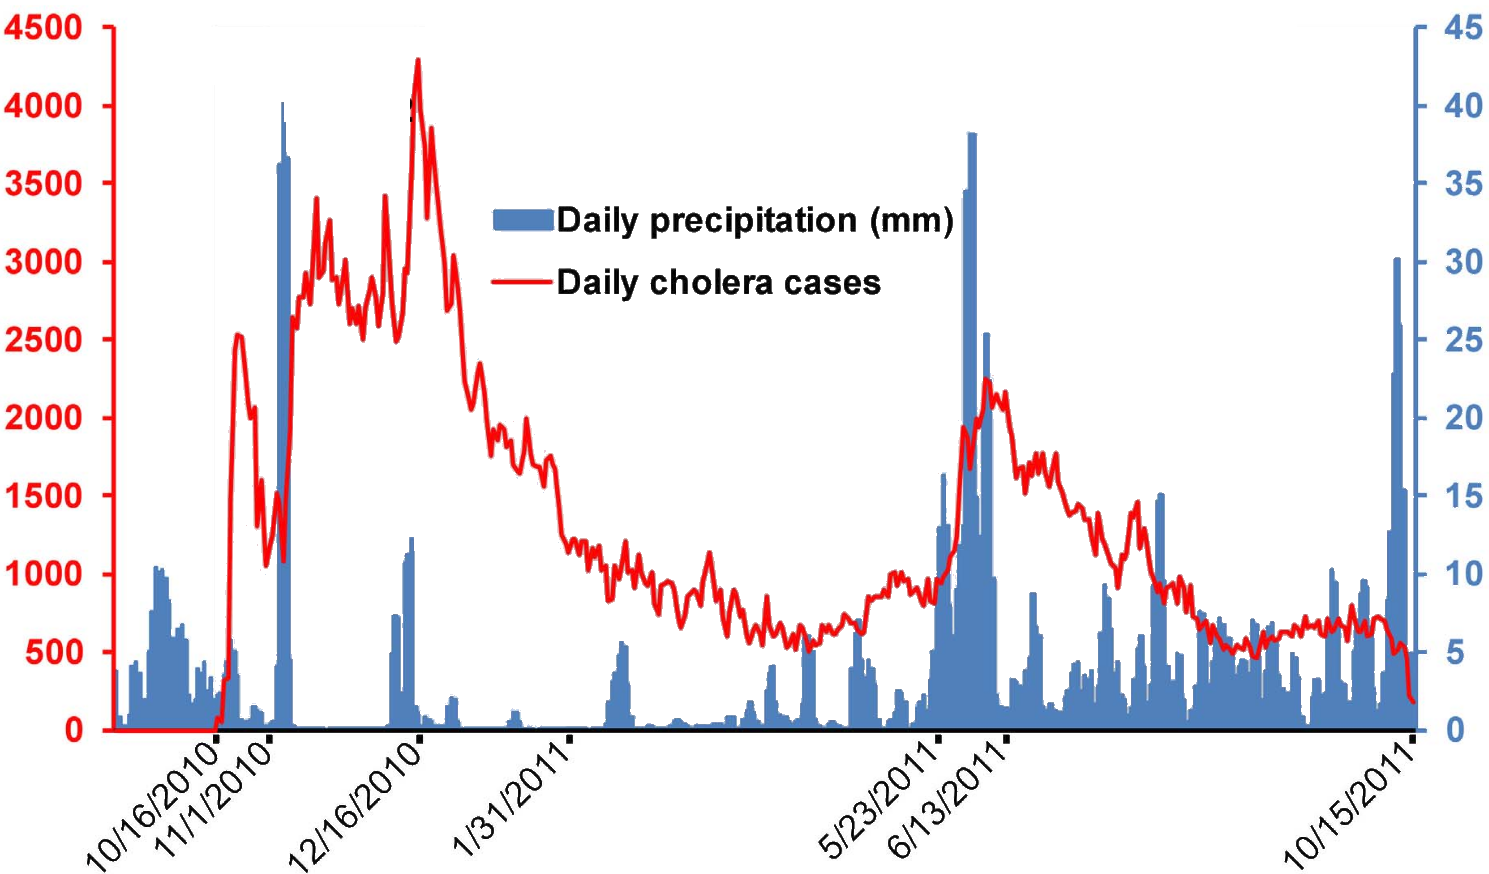
\includegraphics{fig/cholera-rainfall.png}
\margincaption[Similarities between daily cholera incidence and rainfall in Haiti]{\footnotesize Daily cholera cases (red) and daily rainfall (blue) in Haiti from September 15, 2010 to October
16, 2011. It highlights the visual correlation between heavy rainfall event and cholera outbreaks. Adapted from \fullcite{Gaudart:SpatioTemporalDynamicsCholera:2013}.}
\label{fig:rain}
\end{marginfigure}
 Previous studies have highlighted the role of climatic drivers on cholera dynamics, mostly focusing on climate change effects on disease spread\shortcite{Rinaldo:ModelingKeyDrivers:2017,Hashizume:EffectRainfallIncidence:2008,Magny:CholeraOutbreakSenegal:2012,Rodo:ClimateChangeInfectious:2013,Ramirez:NinoClimateCholera:2016,Vezzulli:ClimateInfluenceVibrio:2016} or on the impacts of spatial and temporal heterogeneities\shortcite{Reiner:HighlyLocalizedSensitivity:2012, Baker-Austin:EmergingVibrioRisk:2013, Vezzulli:OceanWarmingSpread:2013, Cash:CholeraShigellosisDifferent:2014,Escobar:GlobalMapSuitability:2015, Vezzulli:EffectsGlobalWarming:2015,Perez-Saez:ClimatedrivenEndemicCholera:2017}. The effect of temperature on cholera transmission has been described (though mainly through the lense of \textit{Vibros} survival and ecology in natural environments), but for rainfall, it remains to be fully elucidated, possibly due to the multiple ways in which it can influence transmission at the local and regional scales\shortcite{Rinaldo:Reassessment20102011:2012,Eisenberg:ExaminingRainfallCholera:2013,Baracchini:SeasonalityCholeraDynamics:2017}. Indeed, intense rainfall events have been shown to alter infection risk through a variety of potential mechanisms, including: flooding, leading to sewage contamination of water sources\shortcite{Ruiz-Moreno:CholeraSeasonalityMadras:2007, Hashizume:EffectRainfallIncidence:2008}; increased hydrologic transport-driven iron availability in environmental waters that enhances pathogen survival and the expression of toxins\shortcite{Lipp:EffectsGlobalClimate:2002,Faruque:SeasonalEpidemicsCholera:2005, Hill:ToxigenicVibrioCholerae:2011}; dry spells inducing persistent low water levels leading to increased use of unsafe water sources\shortcite{Rebaudet:EnvironmentalDeterminantsCholera:2013}; and crowding during strong flood events\shortcite{Reiner:HighlyLocalizedSensitivity:2012}.

Most countries where associations between rainfall and cholera risk have been studied experience endemic cholera transmission. Empirical studies have shown a range of correlations, both positive and negative, endowed with time lags ranging from weeks to months\shortcite{Ruiz-Moreno:CholeraSeasonalityMadras:2007,Emch:SeasonalityCholera1974:2008,Magny:CholeraOutbreakSenegal:2012}. In general, rainfall has been found to increase cholera transmission, but there is evidence of the inverse, possibly due to pathogen dilution\shortcite{Ruiz-Moreno:CholeraSeasonalityMadras:2007}. Such variability reflects the variety of potential mechanisms whereby rainfall may alter infection risk. Similarly, a clear empirical correlation between intense rainfall and enhanced transmission is found in several regions hit by cholera epidemics\shortcite[][but Haiti is treated specifically in the next chapter]{Magny:EnvironmentalSignaturesAssociated:2008,Magny:CholeraOutbreakSenegal:2012,Rebaudet:EnvironmentalDeterminantsCholera:2013,Rebaudet:CholeraCoastalAfrica:2013,Jutla:WaterMarkerMonitored:2013} (fig. \ref{fig:rain}). Results therein showed that at all spatial scales and locations examined, tropical storms were correlated with increased cholera incidence with lags of the order of a few days. As a consequence, accounting for the related forcing of dynamic models resulted in improved fits of reported incidence. 

Properly incorporating the effects of rainfall in mathematical models of cholera transmission is thus paramount to discriminate among the above-mentioned alternative transmission pathways, thus unlocking a predictive framework to evaluate the potentially rainfall-sensitive efficacy of available intervention strategies in endemic and epidemic settings. This becomes  critically important when evaluating the number of averted infections by deploying vaccines, as was done in the aftermath of the passage of Hurricane Matthew\shortcite{Pasetto:RealtimeProjectionsCholera:2017}, or considering optimal deployment in space and time.

The effect of rainfall on indirect cholera transmission has been accounted for in two main fashions in recent mathematical models. On one side, a \textit{contamination}-centered approach suggesting that bursts of infections could be linked to increased contamination of the water compartment\shortcite{Rinaldo:Reassessment20102011:2012}, as in the ECHO model presented in \textsc{Chapter~2}. This process conceptualizes the washout of open-air defecation sites by hydrologic transport. The same `transport' effect may be realized by sewer collectors' overflows. In fact, both mechanisms have the net effect of charging progressively the bacterial concentration in the water reservoir\shortcite{Codeco:EndemicEpidemicDynamics:2001}. Pathogens' loads are washed out from a hydrologic catchment enclosing human settlements and their infective individuals shedding bacteria. Therein, pathogen survival and thus the toxicity of their loads depend on hydrologic residence time distributions\shortcite{Rinaldo:Reassessment20102011:2012,Rinaldo:ModelingKeyDrivers:2017}. Such loads increase as a function of rainfall, which acts as proxy of runoff volumes. The second approach is \textit{exposure}-centered and employs a rainfall-dependent exposure rate subsuming both pathogen availability and the probability of the ingestion of contaminated water during wet spells\shortcite{Eisenberg:ExaminingRainfallCholera:2013}. Although both approaches are physically plausible, they have not been compared directly on the same datasets within a formal statistical framework, which would allow to highlight their respective merits and further recommendations for their use in different settings.

In this chapter, the explanatory power of these different types of rainfall-driven mechanistic models applied to a cholera outbreak in South Sudan is compared. The link between rainfall and cholera during the outbreak recorded in Juba in 2015, when an intra-seasonal peak of cholera cases was recorded possibly in correspondence to intense precipitation events is quantitatively examined. The analysis of the lagged relationship between rainfall rates and revamped cholera incidence is addressed via dynamical compartmental models considered both in deterministic and stochastic versions incorporating both direct (human-to-human) and indirect (water-to-human) disease transmission, and rainfall effects on both contamination and exposure.
\section{Case study: the 2015 cholera outbreak in Juba, South Sudan}\label{sec:data sets}
\begin{figure}\centering
  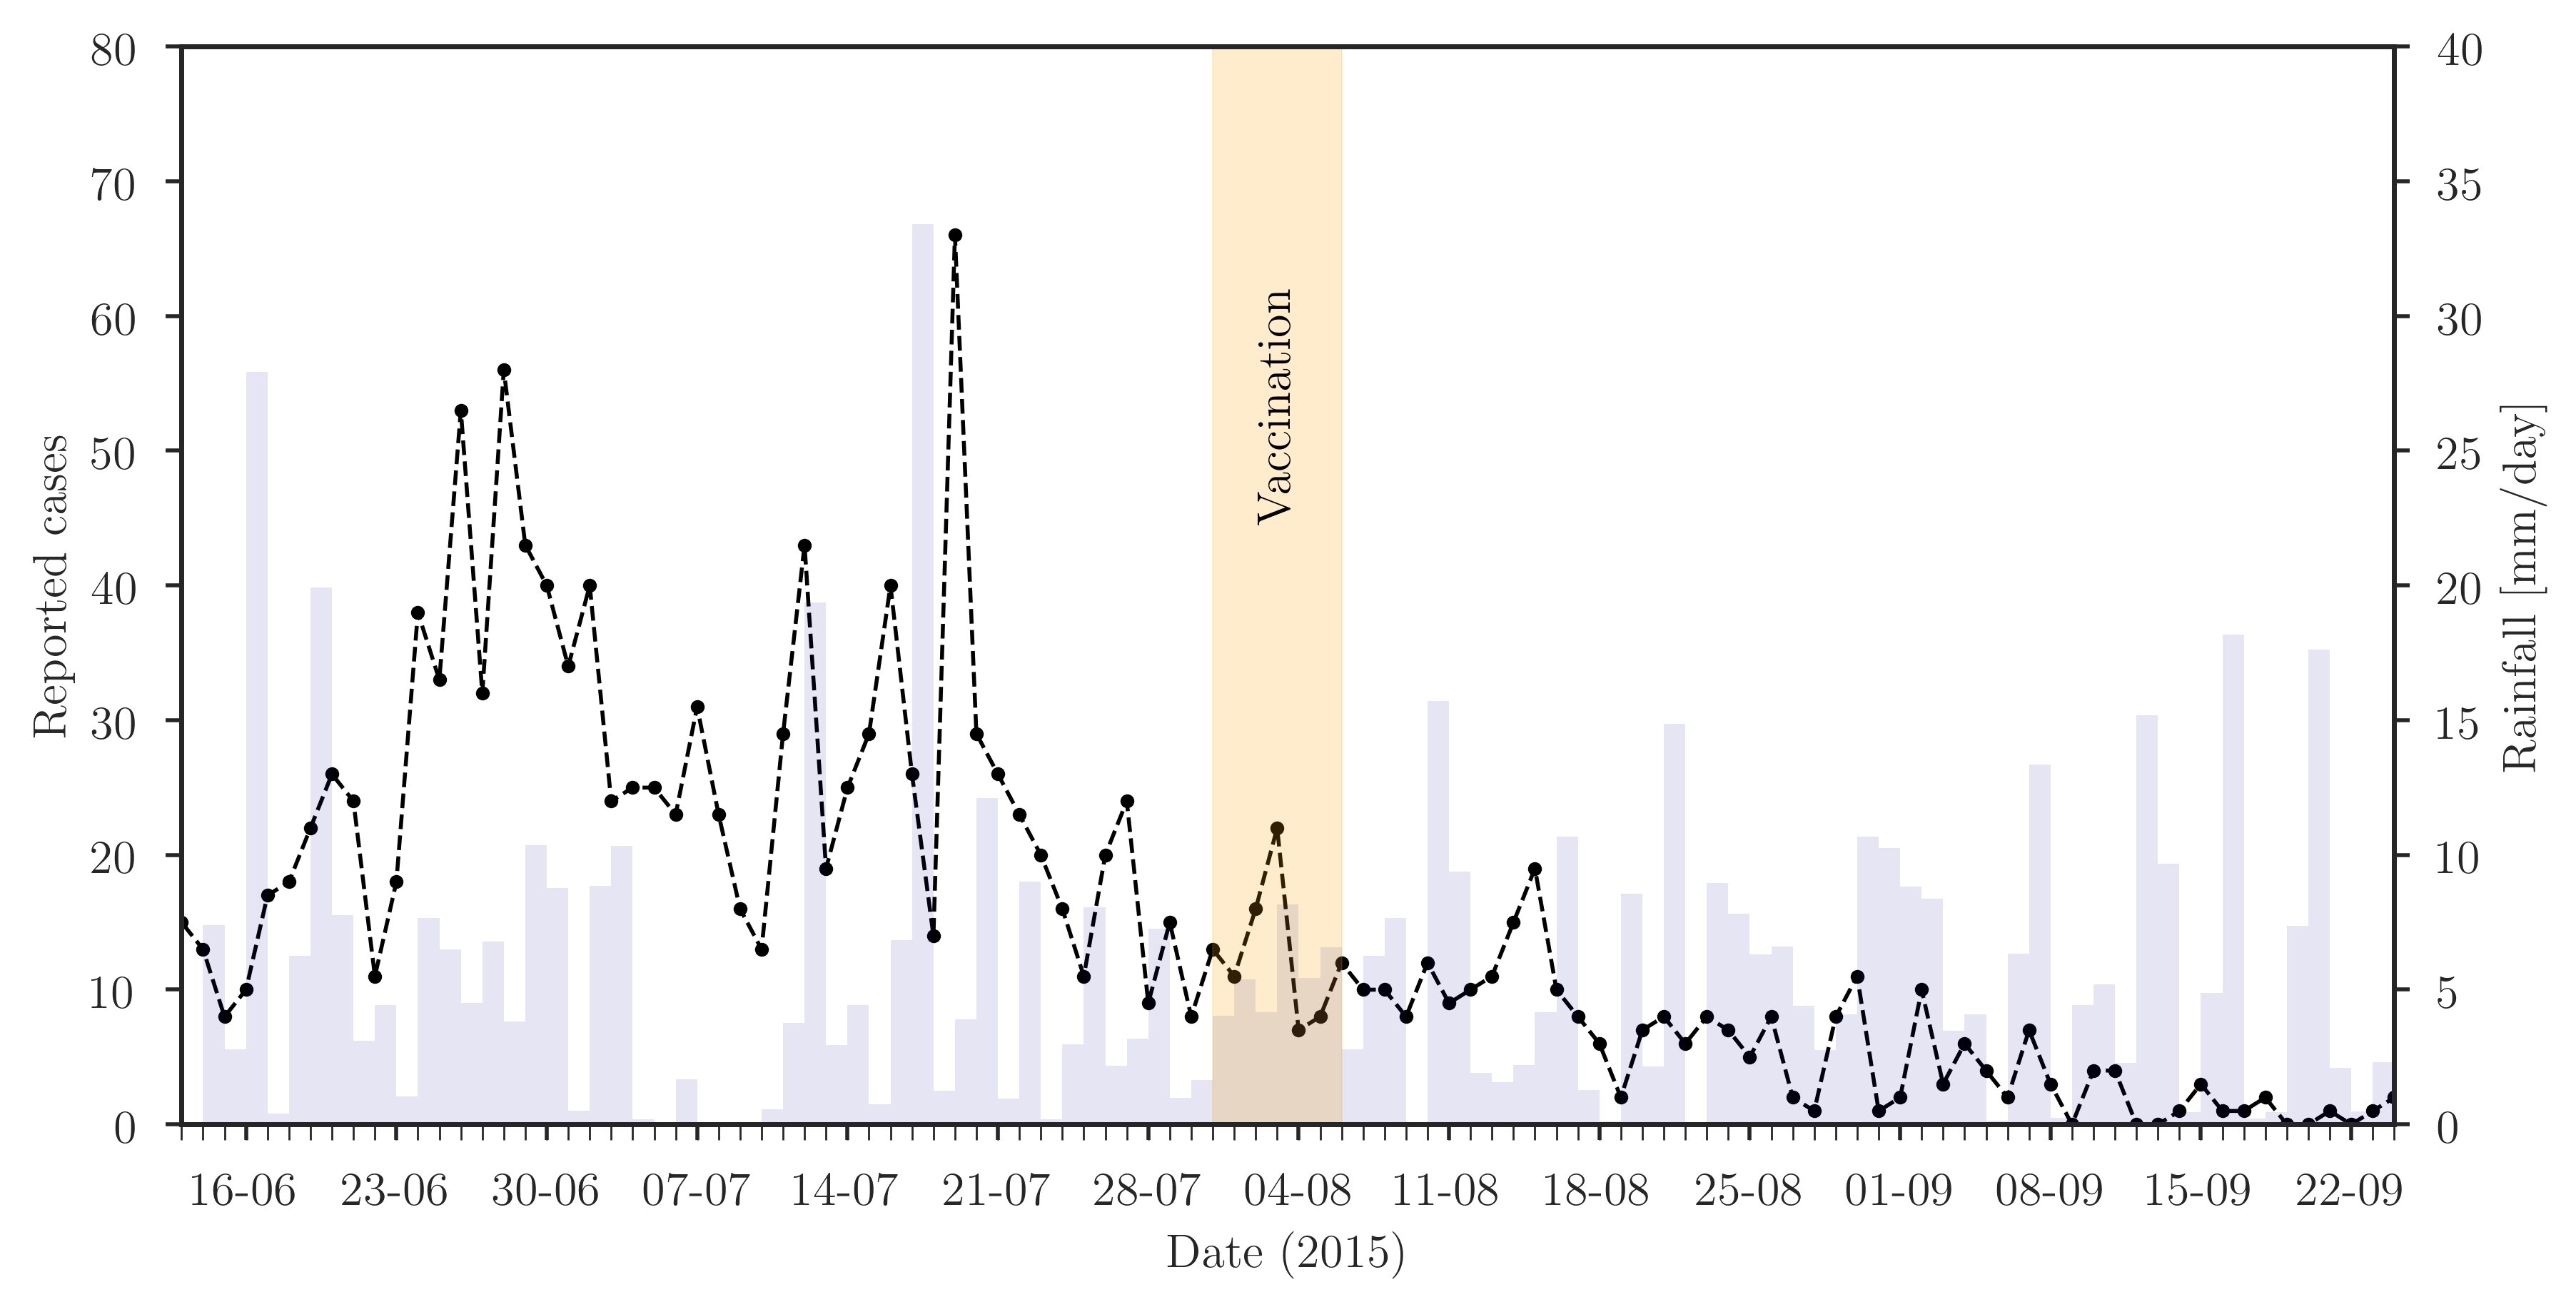
\includegraphics{fig_cholera-rainfall/Lemaitre_ACTROP_2018_42_R1_fig2.png}
  \caption[Cholera cases and precipitation during the 2015 cholera epidemic in Juba][2\baselineskip]{Reported cholera cases (dots) and precipitation (bars) during the 2015 cholera epidemic in Juba. The timing of the vaccination campaign is highlighted in yellow.}\label{fig:report}
\end{figure}
In the past years, South Sudan had been struck by several cholera outbreaks\footnote{More details on the history of cholera in South Sudan are found in: \fullcite{Sciarra:MathematicalModelingCholera:2018}}. Here the analysis focuses on the 2015 outbreak in Juba, when a particular double peak of cholera cases was associated to a strong intra-seasonal precipitation event (fig.~\ref{fig:report}). Access was to granted to epidemiological records for the 2014 and 2015 cholera epidemics that include daily cholera incident cases and hospitalization at the second-lowest administrative level (Payams), reported by the Ministry of Health of South Sudan. The cases in the 7 Payams that constitute the administrative area of Juba have been aggregated to obtain the reported time series for the county level. The population data for Juba county is taken from the South Sudan National Bureau of Statistics\cite[-4\baselineskip]{SSNBS:PopulationProjectionsSouth:2015}. Daily rainfall estimates for years 2014 and 2015 were obtained from the Climate Data Library\cite[-3.5\baselineskip][with a resolution of {0.1}$^\circ$, rainfall was averaged over the study area.]{IRI/LDEO:ClimateDataLibrary:2016}. In 2015, 167'377 OCV doses were distributed in the county of Juba during 6 days of a mass vaccination campaign started on July 31, 2015\cite[-3.2\baselineskip]{Abubakar:FirstUseGlobal:2015,Azman:EffectivenessOneDose:2016,Parker:AdaptingGlobalShortage:2017}, and are taken into account in the model.
%FFN: South Sudan has a lot of one dose
\newpage
\section{Cholera models}
\label{sec:meth}
\subsection{Generalized cholera model}
The proposed model is inspired from the model presented in the previous chapter: we have the susceptible $S$, infected $I$, and recovered $R$ compartments for individuals, with an additional variable $B$ describing the concentration of the bacteria in the environment. Previous modelling exercises had considered rainfall intensity $J(t)$ either to i) multiplicatively increase water \textit{contamination} with bacteria shed by infected  individuals\cite{Bertuzzo:ProbabilityExtinctionHaiti:2016,Pasetto:RealtimeProjectionsCholera:2017}, or ii) assumed that the rainfall multiplicatively increases the \textit{exposure} to contaminated water\cite{Eisenberg:ExaminingRainfallCholera:2013}. A generalized formulation of these cholera-forced models, wherein both formulations are nested, is proposed. It enables the systematic comparison of the effect of rainfall through these two different transmission pathways.

The model described in \textsc{Chapter~1} was designed to deal with weekly data. Here, given the daily temporal resolution at which incidence data was available for the 2015 Juba's epidemic, a compartment of exposed individuals $E$ is added to the model structure. It describe the incubation period: the lag between the time of exposure and the onset of the symptoms. Moreover, in order to account for the vaccination campaigns that were deployed in Juba in August 2015, four compartments ($V^S$, $V^E$, $V^I$, and $V^R$) are added to describe the dynamics of vaccinated individuals and their removal from the pool of susceptibles.

The proposed generalized cholera model is described in fig.~\ref{diagram}, and formulated as:
\marginnote[7\baselineskip]{
\begin{tabular}{ll}
\toprule
     symbol      & signification   \\
    \hline
$\alpha$ & cholera induced mortality\\
$\mu$ & natural mortality\\
$\sigma$ &symptomatic fraction\\
$\gamma$ & infectious period \\
$\rho$ & duration of immunity \\
$\rho_v$ & duration of vaccine protection \\
$\eta$ & vaccine efficacy \\
$\theta$ & shedding rate \\
$\mu_B$ & bacteria decay in water \\
$J(t)$ & rainfall \\
\bottomrule
\end{tabular}\\Reminder of the parameters already described in \textsc{Chapter~1} (p.\pageref{eq:I2}).}

\begingroup
\allowdisplaybreaks
\begin{eqnarray} \label{eq:fullmodel}
S(t) &=& H - I(t) - E(t) - R(t) - V^S(t) - V^E(t) - V^I(t) - V^R(t) \label{eq:S2j} \\
 \frac{dE}{dt} &=& \sigma F(t) S - (\phi + \mu +\nu) E \label{eq:E2j}\\
 \frac{dI}{dt} &=& \phi E - (\gamma + \mu + \alpha) I \label{eq:I2j}\\
 \frac{dR}{dt} &=& (1-\sigma) F(t) S + \gamma I - (\rho + \mu+\nu) R \label{eq:R2j}\\
 \frac{dB}{dt} &=& - \mu_B B +\theta\left[1 + f_{\mathcal{c}}\left(J(t)\right) \right] (I+V^I)\label{eq:B2}\\
\frac{dV^S}{dt} &=& \nu S - \mu V^S+ \rho_{v} V^R - (1-\eta) F(t) V^S \label{eq:VS2j}\\
 \frac{dV^E}{dt} &=& \nu E + \sigma (1-\eta) F(t) V^S-(\phi + \mu) V^E \label{eq:VE2}\\
 \frac{dV^I}{dt} &=&  \phi V^E -(\gamma + \alpha + \mu) V^I \label{eq:VI2j}\\
 \frac{dV^R}{dt} &=& \nu R -(\mu +\rho_{v})V^R +\gamma V^I +(1-\sigma) (1-\eta) F(t) V^S\label{eq:VR2j}\; ,
\end{eqnarray}
\endgroup
where $F(t)$ takes into account both human-to-human transmission and nonlinear water-to-human transmission:
\begin{equation}
  F(t) = \beta_B \underbrace{ \left[\frac{B}{K + B} \right] \bigg(1+f_{\mathcal{e}}\left(J(t)\right)\bigg)}_{\text{indirect transmission}} + ~\beta_{I} \underbrace{\frac{(I+V^I)}{H}}_{\text{direct transmission}}.
\label{eq:force2}
\end{equation}
 The notation is consistent with \textsc{Chapter~1} and we refer the reader to the description of the processes provided on \pageref{eq:I2}, and reminded in the margin table. In addition to tge previously decribed dynamics, exposed individuals become symptomatic infected at a rate $\phi$, which corresponds to an average incubation period of $1/\phi\approx$ 1.5 days\cite{Azman:IncubationPeriodCholera:2013}. As few reliable data on changes in Juba's population are available for the years of interest, the total population $H$, is assumed to be constant, as in \eqref{eq:S2j}. 
 
Moreover, the effect of rainfall is more precisely described. Functions $f_{\mathcal{c}}\left(J(t)\right)$ and $f_{\mathcal{e}}\left(J(t)\right)$ account for the rainfall effect respectively by increasing the bacteria contamination in the water reservoir or directly through amplifying the exposure in the force of infection.
\begin{figure}
  \centering
  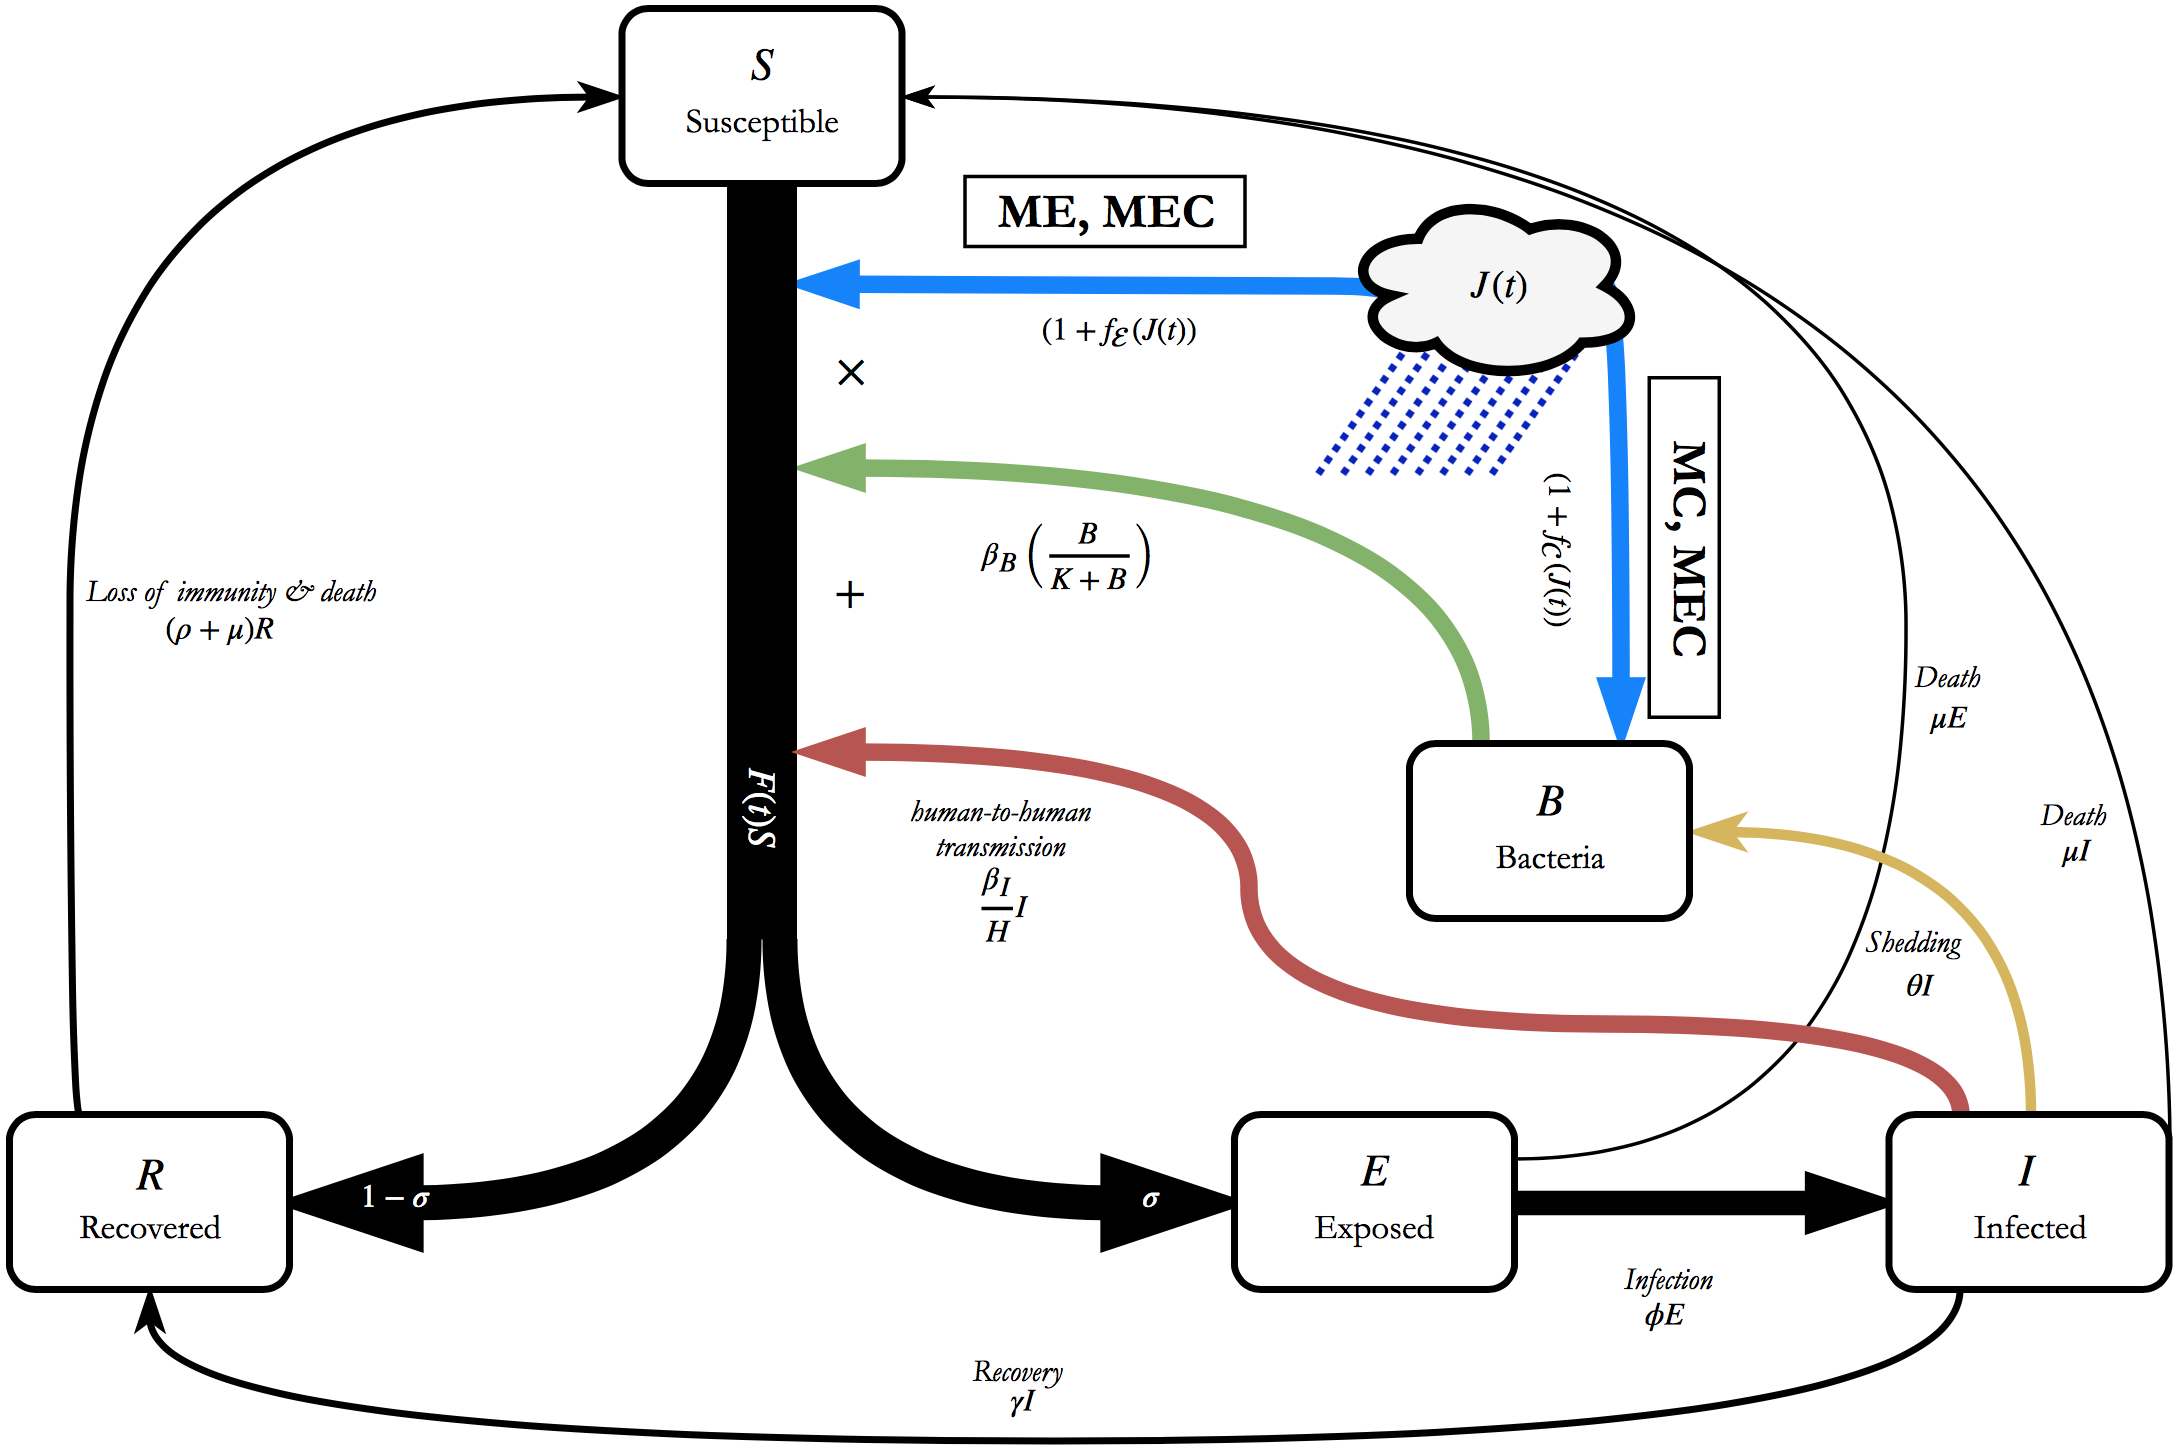
\includegraphics{fig_cholera-rainfall/Lemaitre_ACTROP_2018_42_R1_fig1.png}
  \caption[Transition diagram for the competing cholera models]{Transition diagram for the different cholera models considered, with the different variations \textsc{me}, \textsc{mr}, and \textsc{mec} indicated.}
  \label{diagram}
\end{figure}
With the objective of assessing the importance of rainfall on cholera transmission, a generalization of the linear relation found in the litterature\footnote{Specifically the reference exposure \parencite{Eisenberg:ExaminingRainfallCholera:2013} and contamination \parencite{Rinaldo:Reassessment20102011:2012} models.} is proposed, by using a nonlinear function form for  $f_{\mathcal{c,e}}\left(J(t)\right)$:
\begin{equation}
    f_{\mathcal{c,e}}\left(J(t)\right)=\lambda_{\mathcal{c,e}} \left(\frac{J(t)}{\max_t J(t)}\right)^{\alpha_{\mathcal{c,e}}}
    \label{eq:nonlinear_rain}
\end{equation}
\begin{marginfigure}
	\centering
	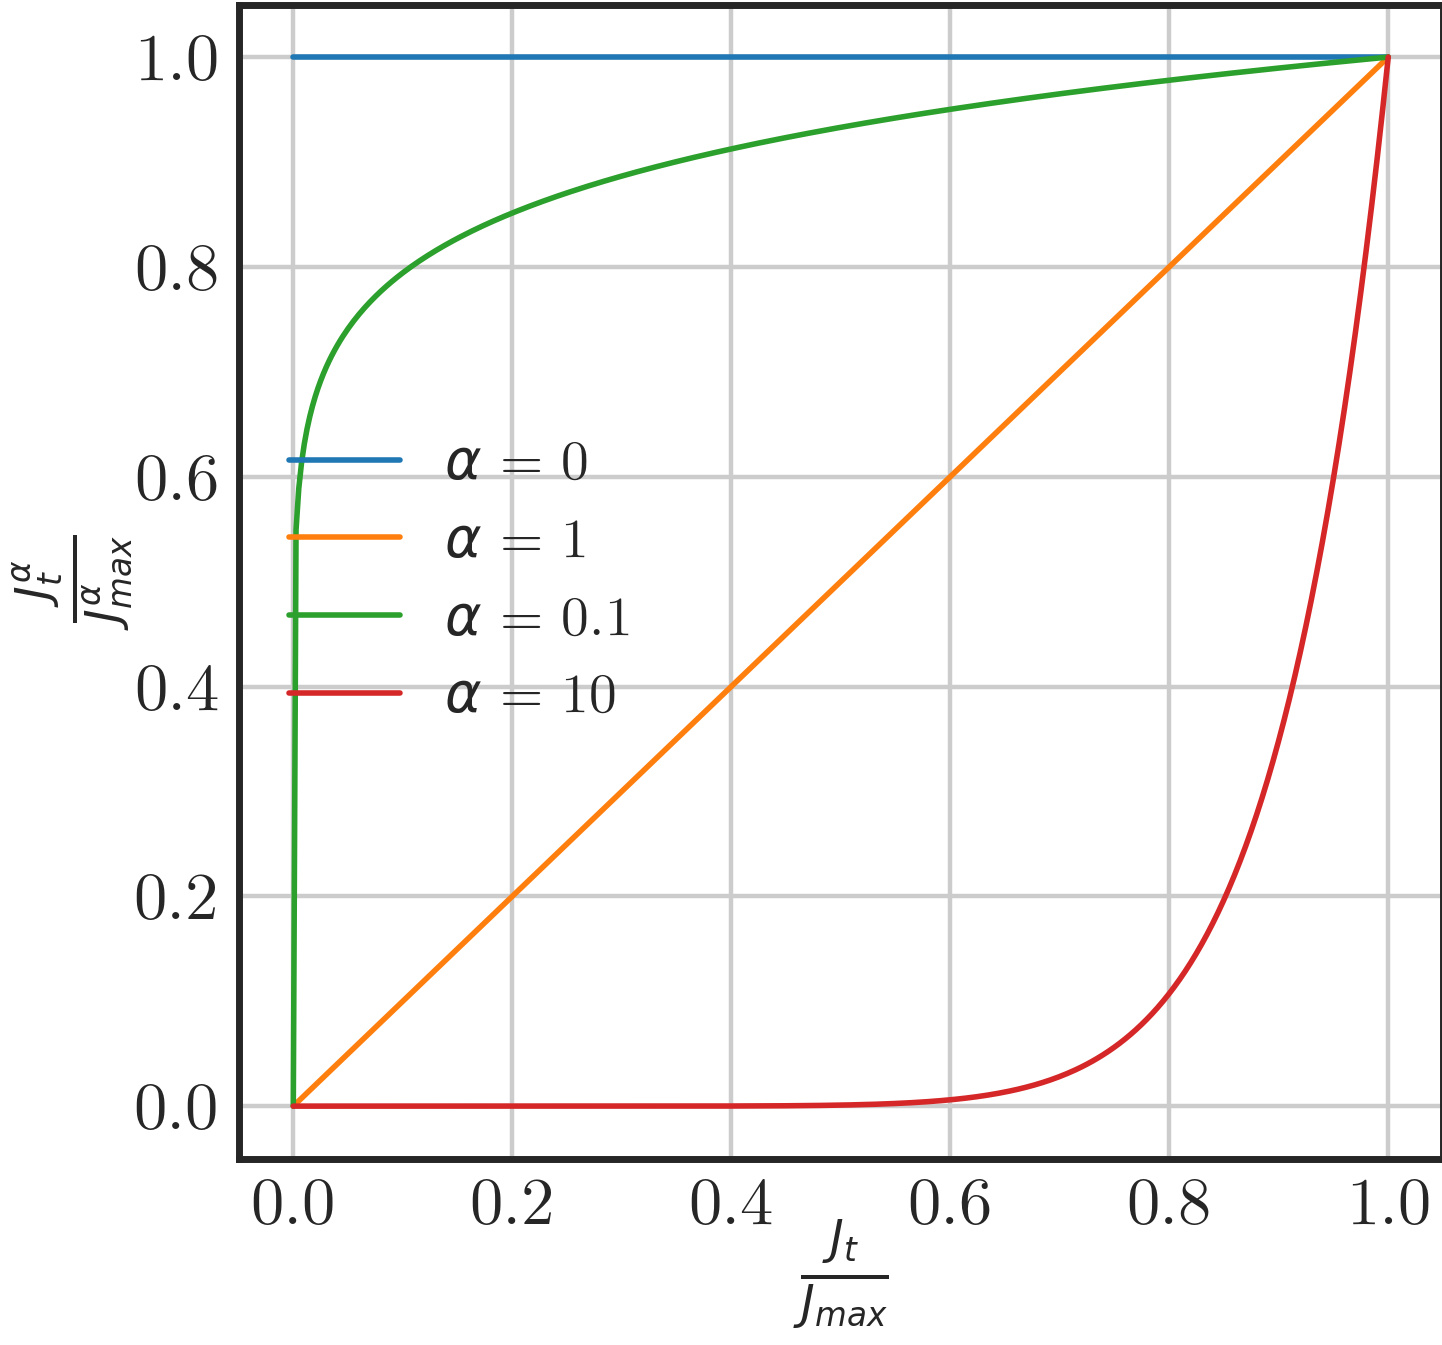
\includegraphics{fig_cholera-rainfall/alpha.png}
	\margincaption[Non-linear rainfall effect on transmission]{$\left(\frac{J_t}{J_{max}}\right)^\alpha$ for different values of $\alpha$. For $\alpha = 1$, the linear model described in previous works is obtained, and larger $\alpha$ corresponds to an increased relative importance of heavy rainfall events.}
	\label{fig:alpha}
\end{marginfigure}
where the subscripts $_\mathcal{c,e}$ respectively denote the effect of rainfall on exposure and contamination, $\max_t J(t)$ is the maximum recorded rainfall intensity during the epidemic, and the $\alpha_{\mathcal{c,e}}\ge0$ controls for the relative importance of different rainfall intensities in their effect on the force of infection. Indeed, since the ratio $\frac{J(t)}{\max_t J(t)} \in [0,1]$, for $\alpha_{\mathcal{c,e}} \gg 1$ the ratio will tend to $0$ for all small precipitation events, leaving only the effect of the strongest events, whereas for $\alpha_{\mathcal{c,e}} < 1$ all precipitation events will be assigned a similar weight in the force of infection (fig. \ref{fig:alpha}). The formulations found in litterature are recovered by setting $\alpha_{\mathcal{c,e}} = 1$. The flexibility allowed by eqn.~\eqref{eq:nonlinear_rain} allows to discriminate between rainfall effects along a continuum from acting on disease transmission regardless of intensity to a threshold-like effect for the largest events which could be associated to severe flooding causing damages to the city's water and sanitary system, for instance leading to sewer overflow.

\subsection{Competing transmission models}
The relevance of the two rainfall-driven transmission pathways is assessed here by comparing the following models:
\begin{itemize}
 \item \textsc{mn} SIRB model without rainfall: $\lambda_{\mathcal{c}} = \lambda_{\mathcal{e}} = 0$, $\beta_{I} = 0$, as the null hypothesis for the importance of rainfall.
  \item \textsc{mc} SIRB model where for rainfall enhances the \textit{contamination} of the water reservoir: $\lambda_{\mathcal{e}} = 0$, $\beta_{I} = 0$. 
  \item \textsc{me} SIRB model where rainfall increases the \textit{exposure} to bacteria: $\lambda_{\mathcal{c}} = 0$, $\beta_{I} = 0$. 
  \item \textsc{mec} SIRB model combining both approaches \textsc{mc} and \textsc{me} ($\beta_{I} = 0$). Both ways of accounting rainfall play a role simultaneously.
\end{itemize}
\marginnote[-8\baselineskip]{\textsc{me} models uses a similar transmission pathway as in \textcite{Eisenberg:ExaminingRainfallCholera:2013}, whereas \textsc{mc} models were described in \textcite{Rinaldo:Reassessment20102011:2012}. These models were adapted to the generalized configuration, \eg in eqn.~\eqref{eq:force2} precipitation enters in the term $\left(1+f_E \left(J(t)\right)\right)$ which entails water-to-human transmission also when $J(t)=0$, unlike the published version. The steps take to adapt these models are shown in the postprint supplementary, section S.1.}
\begin{table}[h!]
\centering
\begin{tabular}{lccccc}
\toprule
     Model       & $\lambda_{\mathcal{c}}$ & $\alpha_\mathcal{c}$ & $\lambda_{\mathcal{e}}$ & $\alpha_\mathcal{e}$ & $\beta_I$   \\
    \hline
    \textsc{mn} &       --    &    --   &       --      &       --      &  -- \\
    \textsc{mnh} &     --      &   --    &    --         &        --     &   $\times$ \\
    \textsc{mc} &      $\times$  &  $\times$  &     --        &       --      &  -- \\
    \textsc{me} &         --  &   --    &      $\times$    &   $\times$        & --  \\
    \textsc{mch}&      $\times$  &  $\times$  &      --       &     --        &$\times$ \\
    \textsc{meh}&        --   &  --     &      $\times$    &   $\times$        &$\times$ \\
    \textsc{mec}&      $\times$ &  $\times$  &      $\times$    &    $\times$      & --\\
    \textsc{mech}&      $\times$ &  $\times$  &      $\times$    &    $\times$       &   $\times$ \\
\bottomrule
\end{tabular}
\caption[Parameters considered in the eight compared models]{Parameters considered in the eight compared models.  $\lambda$ and $\alpha$ characterize the functional forms considering the precipitation eqn.~\eqref{eq:nonlinear_rain}. $\beta_I$ is the exposure for human-to-human transmission. A dash -- indicate that the parameter is set to zero, whereas a cross $\times$  indicate that the parameter is used.}
\label{tab:models}
\end{table}

 For each model is explored the possibility of adding explicitly direct, human-to-human transmission ($\beta_{I} > 0$), which is indicated with an \textsc{H} at the end of the model name: \textsc{mnh}, \textsc{mch}, \textsc{meh}, and \textsc{mech}. The different parameters associated with the considered models are summarized in tab.~\ref{tab:models}.

 The eight models are compared on the basis of their ability to match the time series of daily reported cases during the cholera epidemic in Juba of 2015. In the postprint, tab. S.1 summarizes which parameters are calibrated for each model and their prior distribution. The degrees of freedom of the models, $n_p$, vary from $n_p=7$ for \textsc{mn} to $n_p=12$ for \textsc{mech}. Given the low number of daily reported cases and their ensuing variability, a stochastic equivalent is also implemented\footnote[][-8\baselineskip]{The sole difference in formulation is the introduction of overdispersion in the infection process. The force of infection is multiplied by a time-continuous white noise process, as detailled in the eqns. \eqref{eqn:sta}--\eqref{eqn:stb}.} of the deterministic ODE system, eqns. \eqref{eq:fullmodel}-\eqref{eq:VR2j}, formulated as a continuous time partially observed Markov process model, accounting for both demographic and disease transmission stochasticities\cite{Breto:TimeSeriesAnalysis:2009}. The formulation of the stochastic model is left in the \textsc{Appendix}, eqn. \eqref{eq:stochsys} on p. \pageref{eq:stochsys}.

\subsection{Models calibration}
\marginnote{For details about fixed and calibrated parameters, along with prior and posterior distributions, the reader is referred to the supplemental information of \fullcite{Lemaitre:RainfallDriverEpidemic:2019}.}
\paragraph{Initial conditions} The past history of cholera epidemics in South Sudan, and particularly in Juba, plays an important role in the determination of the size of susceptible and recovered compartments at the beginning of the 2015 epidemic. These two compartments are also largely impacted by the rate of immunity loss $\rho$ of the recovered individuals, and by the probability of asymptomatic infection $1-\sigma$\footnote[][2\baselineskip]{values in literature range between $\sigma=0.5$, meaning one asymptomatic per each symptomatic infected, to less than $\sigma=0.01$, corresponding to more than 99 asymptomatic infected per each symptomatic infected \parencite{Fung:CholeraTransmissionDynamic:2014}.}. The initial conditions must therefore be estimated for each parameter set considered during calibration.

 
 To take into account the uncertainty associated with the immunity landscape of Juba, the initial number of recovered individuals in April 2014 is calibrated for each model. Then, the detailed daily data of suspected cases during 2014 is used to estimate the associated number of recovered individuals at the start of the 2015 epidemic. Suspected cases in 2014 are scaled to the reporting fraction and  undergo an exponential decay with average time of immunity loss $1/\rho$\footnote{Something similar has been done in \parencite{Pasetto:RealtimeProjectionsCholera:2017}.}. Simulations are then initialized on June 5, 2015 considering two exposed individuals, two infected, and the associated steady-state bacteria concentration. 
 
\paragraph{Calibration} Calibration of the deterministic model is performed using a Markov Chain Monte Carlo based algorithm\footnote{Differential Evolution Adaptive Metropolis, \textsc{dream}: \parencite{Vrugt:MarkovChainMonte:2016}, which was developed to explore high-dimensional parameter spaces. Given the parameters' prior distribution, \textsc{dream} searches and selects new samples in the posterior distribution by using multiple \textsc{mcmc} chains that run in parallel and that jointly contribute to the computation of the proposal parameter samples. \textsc{Mcmc} chains  converge toward the posterior probability distribution based on the log-likelihood function of the data given the model output.} , which draws samples from the posterior distribution of the parameters.
Inference on the stochastic model is performed using a frequentist iterated filtering algorithm\footnote{MIF, an algorithm proposed by \parencite{Ionides:InferenceDynamicLatent:2015}, which is a frequentist-based approach for identifying the maximum likelihood estimation. It has proved successful even for a range of complex models of cholera dynamics \parencite{King:InapparentInfectionsCholera:2008,Baracchini:SeasonalityCholeraDynamics:2017}. The MIF2 algorithm, which employs iterated Bayes maps, is implemented in the R package \texttt{pomp} \parencite{King:StatisticalInferencePartially:2015}. %For this exercise, it is configured using 120 initial parameter vectors for each model, built using Sobol sequences over the parameter bounds.
}. Both model were fit against the daily reported cases accounting for over- or under- reporting, and assuming a Poisson likelyhood\shortcite{Camacho:CholeraEpidemicYemen:2018}. Each datapoint at reporting date $t_i$,  $y_{t_i}$, is assumed to belong to a Poisson distribution centered on the modeled incidence $C_{t_i}$\footnote{$C_{t_i}$ is computed as in  eqn. \eqref{eq:C}, but for the $E \rightarrow I$ transition. For the deterministic model: $ C_{t_i} = \int_{t_i}^{t_{i+1}} \phi \left(E(t) + V^E(t)\right) dt$. For the stochastic model the reporting process is described in eqn. \eqref{eq:stochrep}.
% $ C_{t_i} = [N_{EI}(t_{i+1}) - N_{EI}(t_i)] + [N_{V^EV^I}(t_{i+1}) - N_{V^EV^I}(t_i)] $, where $N_{AB}$ denotes the stochastic counting process of transitions between classes $A$ and $B$ .
} and its associated parameter vector $\boldsymbol{\theta}$ altered by the reporting rate $\epsilon$, as:
\begin{equation}
 y_{t_i}  \sim \text{Poisson}\left(\epsilon \,C_{t_i}(\boldsymbol{\theta})\right), \; \epsilon > 0,
 \label{eq:obs}
\end{equation}
 Models were then compared using the Bayesian Information criterion (BIC), Bayes factors, and the likelihood ratio test for the nested models.
 
 
\section{Results}

\subsection{Model selection of the rainfall effects on cholera transmission}
The summary statistics of the deterministic and stochastic models considered in the study are given in tab.~\ref{tab:stats}. Overall, the stochastic models outperform their deterministic counterparts for all model structures by $\approx 40$ log-likelihood units. Both model types agree in the significance of rainfall in explaining the time series of daily reported cases, in particular through the increased exposure pathway, although the specific ordering of the models differs between model types. The BFs for the deterministic models suggest a strong support for model \textsc{mec}, followed by model \textsc{me} ($BF^{-1}_{ME,MEH} = 0.16$), with very little support for all other models ($BF^{-1}_{\boldsymbol{\cdot},MEH}< 10^{-2}$ for all other models than ME). For the stochastic model, the BFs estimated with the BIC suggest the strongest support for model \textsc{me}, with the basic SIRB model coming in second with 5 times less evidence ($BF^{-1}_{MN,ME} \approx 0.15$). 
\begin{table}[h!]
\centering
\small
\begin{tabular}{lcccccccc}
  \toprule
  & \multicolumn{4}{c}{Deterministic} & \multicolumn{4}{c}{Stochastic} \\
    \cmidrule(rl){2-5}\cmidrule(rl){6-9}
  Model & $n$ & $\hat{\ell}$ & BIC & ${BF}^{-1}$ & $n$ & \makecell{$\hat{\ell}$ \vspace{-.1cm} \\ \scriptsize{(s.e.)}}  & BIC  & $BF^{-1}$ \\ 
  \cmidrule(rl){2-5}\cmidrule(rl){6-9}
  \textsc{mn} &   7 & -368.62 & 770.27 & 3.1E-05 &   8 & \makecell{-326.45 \vspace{-.1cm} \\ \scriptsize{(0.105)}} & 690.65 & 1.5E-01 \\ 
   \textsc{mnh} &   8 & -368.95 & 775.64 & 1.1E-09 &   9 & \makecell{-327.52\vspace{-.1cm} \\ \scriptsize{(0.052)}} & 697.51 & 4.7E-03 \\ 
   \textsc{mc} &   9 & -358.32 & 759.11 & 5.5E-03 &  10 & \makecell{-323.50\vspace{-.1cm} \\ \scriptsize{(0.037)}} & 696.01 & 2.5E-02 \\ 
   \textsc{mch} &  10 & -359.06 & 765.30 & 1.7E-04 &  11 & \makecell{-324.89\vspace{-.1cm} \\ \scriptsize{(0.041)}} & 701.68 & 5.9E-04 \\ 
   \textsc{me} &   9 & -356.96 & \textsc{756.40} & 1.6E-01 &  10 & \makecell{\textsc{-319.81}\vspace{-.1cm} \\ \scriptsize{(0.035)}} & \textsc{687.38} & \textsc{1} \\ 
   \textsc{meh} &  10 & -358.06 & 763.30 & 6.3E-04 &  11 & \makecell{-320.64\vspace{-.1cm} \\ \scriptsize{(0.030)}} & 693.18 & 4.1E-02 \\ 
   \textsc{mec} &  11 & \textsc{-356.87} & 765.64 & \textsc{1} &  12 & \makecell{-320.17\vspace{-.1cm} \\ \scriptsize{(0.031)}} & 696.96 & 6.2E-03 \\ 
   \textsc{mech} &  12 & -357.55 & 771.73 & 2.4E-06 &  13 & \makecell{-320.38\vspace{-.1cm} \\ \scriptsize{(0.024)}} & 702.09 & 4.8E-04 \\ 
   \bottomrule
\end{tabular}
\caption[Model comparison statistics]{Model comparison statistics. For each model is reported its number of parameters $n$, the associated estimated log-likelihood $\hat{\ell}$ (and its Monte Carlo standard error for the stochastic model), and the inverse of the Bayes Factor ($BF^{-1}$) with respect to the model with the largest evidence. The BFs for the deterministic models were computed directly from the parameters posteriors, whereas for the stochastic models they were estimated with the Bayesian Information Criterion (BIC) as $BF_{i} \approx e^{\frac{1}{2} \left( BIC_i - BIC_{min}\right)}$. The BIC for the deterministic models was computed using the maximum log-likelihood value visited with the MCMC algorithm across chains.}\label{tab:stats}
\end{table}
When considering only the BIC, model \textsc{me} ranks first for both the deterministic and the stochastic formulations. Interestingly, all models that include human-to-human transmission present smaller or equal log-likelihoods than their counterparts with only the bacteria compartment, which suggests that the data does not support both environmental and human-to-human transmission within the set of the models considered here.

The results of the nested LR-tests confirm the statistical significance of including rainfall in the cholera transmission models, with the effect on exposure better supported by the data in both model types than the effect on contamination. In the deterministic case, the extension of the basic SIRB (model \textsc{mn}) with rainfall effects were significant for all direct comparisons (fig.~\ref{fig:lltests},\textsc{a}). The addition of human-to-human transmission was not significant mostly due to the above-mentioned lower estimate of the log-likelihood in these models. When considering only a single effect of rainfall (either increasing exposure or contamination), \textsc{me} outperforms \textsc{mc} in terms of likelihood for the same number of parameters. Interestingly, the inclusion of rainfall-induced contamination in model \textsc{me} is rejected due to the very limited increase of the estimated log-likelihood of \textsc{mec}, in contrast with the BFs favouring the latter. Model \textsc{me} is thus the one retained by the LR-tests in the deterministic set of models. In the case of the stochastic models, the LR-tests also highlight the importance of the effect of rainfall on exposure rather than on contamination (fig.~\ref{fig:lltests},\textsc{b}). In fact, the much stronger performance of \textsc{mn} in comparison with its deterministic counterpart relative to all other model structures imposes a stronger condition for retaining additional transmission processes. Indeed, both models \textsc{mc} and \textsc{mch} were rejected when compared to \textsc{mn}, thus only models with rainfall-driven exposure were retained. As in the deterministic case, model \textsc{me} is the one finally retained due to the lack of significance of the inclusion of additional transmission processes. Note that the conclusion based on the LR-tests for the deterministic models should be taken with caution because the \textsc{mcmc} algorithm used for calibration does not directly aim at maximizing the likelihood, but rather at sampling from the posterior distribution of the parameters given the data and the model. Moreover, the best likelihood visited by the chains when sampling the posteriors that are used in the LR-tests is not a formal estimate of the models' likelihood. However, the fact that the LR-tests applied to both model types agree with the selection of \textsc{me} supports their use in both cases.
\begin{figure*}
    \centering
    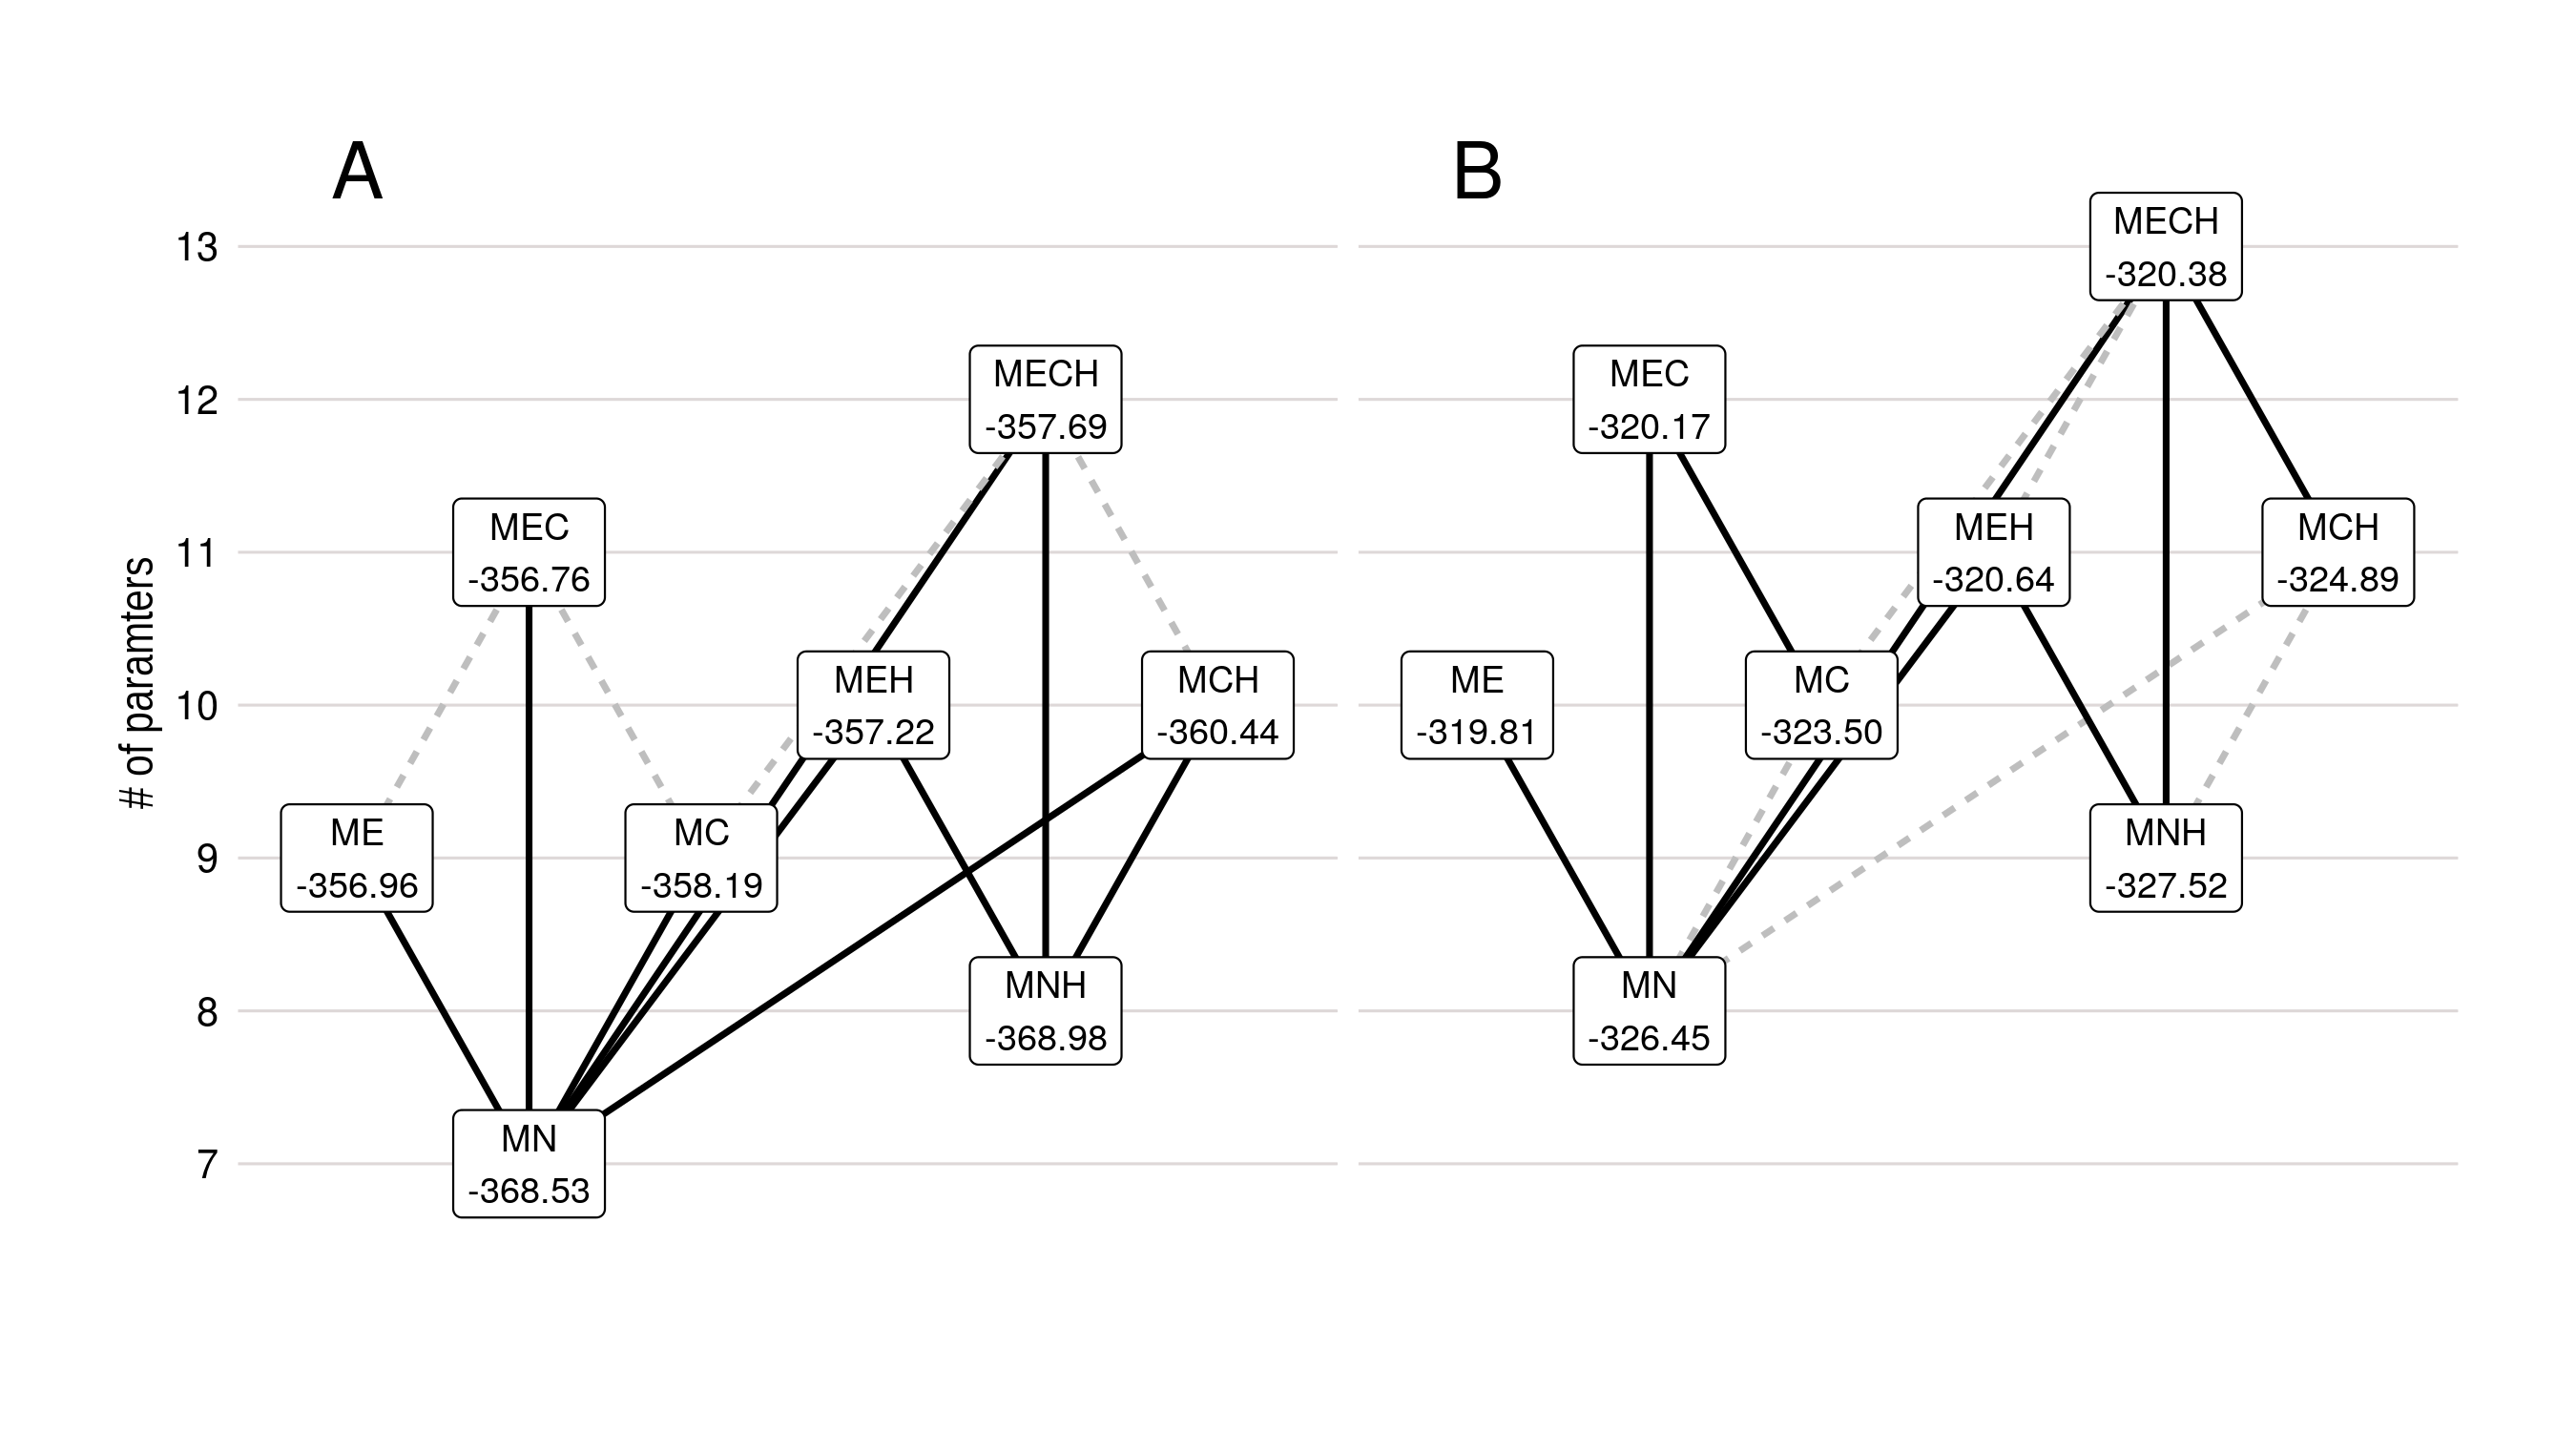
\includegraphics[width = \textwidth, trim = 11mm 19mm 10mm 12mm, clip]{fig_cholera-rainfall/Lemaitre_ACTROP_2018_42_R1_fig3.png}
    \caption[Likelihood ratio tests of model nesting]{Likelihood ratio tests of model nesting. The LL-tests were computed for each nested pair of models $\{\mathcal{M}_0, \mathcal{M}_1\}$, with parameter vectors $\boldsymbol{\theta}^0,\boldsymbol{\theta}^1$, for which at least on of the parameters that is not null is $\boldsymbol{\theta}^1$ is equal to $0$ in $\boldsymbol{\theta}^0$. Each model is labeled with its associated estimated maximum log-likelihood value, $\hat{\ell}$, for the deterministic (A) and the stochastic (B) models, and linked based on whether the likelihood ratio is significantly (full black lines) or not (dashed gray lines) at the 5\% level. The absence of lines indicates a lower $\hat{\ell}$ for the more complex model.} 
    \label{fig:lltests}
\end{figure*}


Both statistical methods for model comparison therefore agree about the importance of the effect of intra-seasonal rainfall on the exposure to transmission during the 2015 cholera epidemic in Juba. For the deterministic type of models the BFs suggest a stronger support for model \textsc{mec}, and the LR-tests for \textsc{me}, whereas for the stochastic models both the BIC-based estimates of BFs and the LR-tests favor \textsc{me}. 

\subsection{Intra-seasonal rainfall events and the 2015 Juba epidemic}

The comparison between the estimated output cases computed by the basic SIRB model (\textsc{mn}) and the most significant rainfall-based processes (\textsc{mec} and \textsc{me} for the deterministic and stochastic types, respectively) highlight the importance of rainfall in retrieving the second epidemiological peak (fig.~\ref{fig:sim}). Both deterministic and stochastic models fit well the general trend of the data, but they clearly underestimate the large number of reported cases on the 19th of July (65 cases). Instead, the more complex models \textsc{me} and \textsc{mec} follow the SIRB dynamics and then are forced by the precipitation occurred in the 18th of July (33 mm/d)  toward the epidemiological peak. 
%

Model calibration results suggest that precipitations with smaller intensities did not have a strong impact on cholera transmission during the 2015 epidemic in Juba. Indeed, the exponents $\alpha_{\mathcal{c}}$ and $\alpha_{\mathcal{e}}$ were found to be systematically larger than 1. %  (as shown by posteriors of the deterministic models in fig. S.2 and the Monte Carlo confidence intervals for the stochastic \textsc{me} in fig. S.4 of the SI) --> appendix or not ? DECISION
  Thus, in the considered epidemic, the nonlinear function used to account for rainfall in the model, eqn.~\eqref{eq:nonlinear_rain}, helps isolating the contribution of the largest rainfall.

The best measures of fit computed for the stochastic \textsc{me} (see tab.~\ref{tab:stats}) are thus explained by a larger sensitivity to precipitation, which causes the match between the mean of the simulated cases and the data during the second peak.

\begin{figure}[ht]
    \centering
    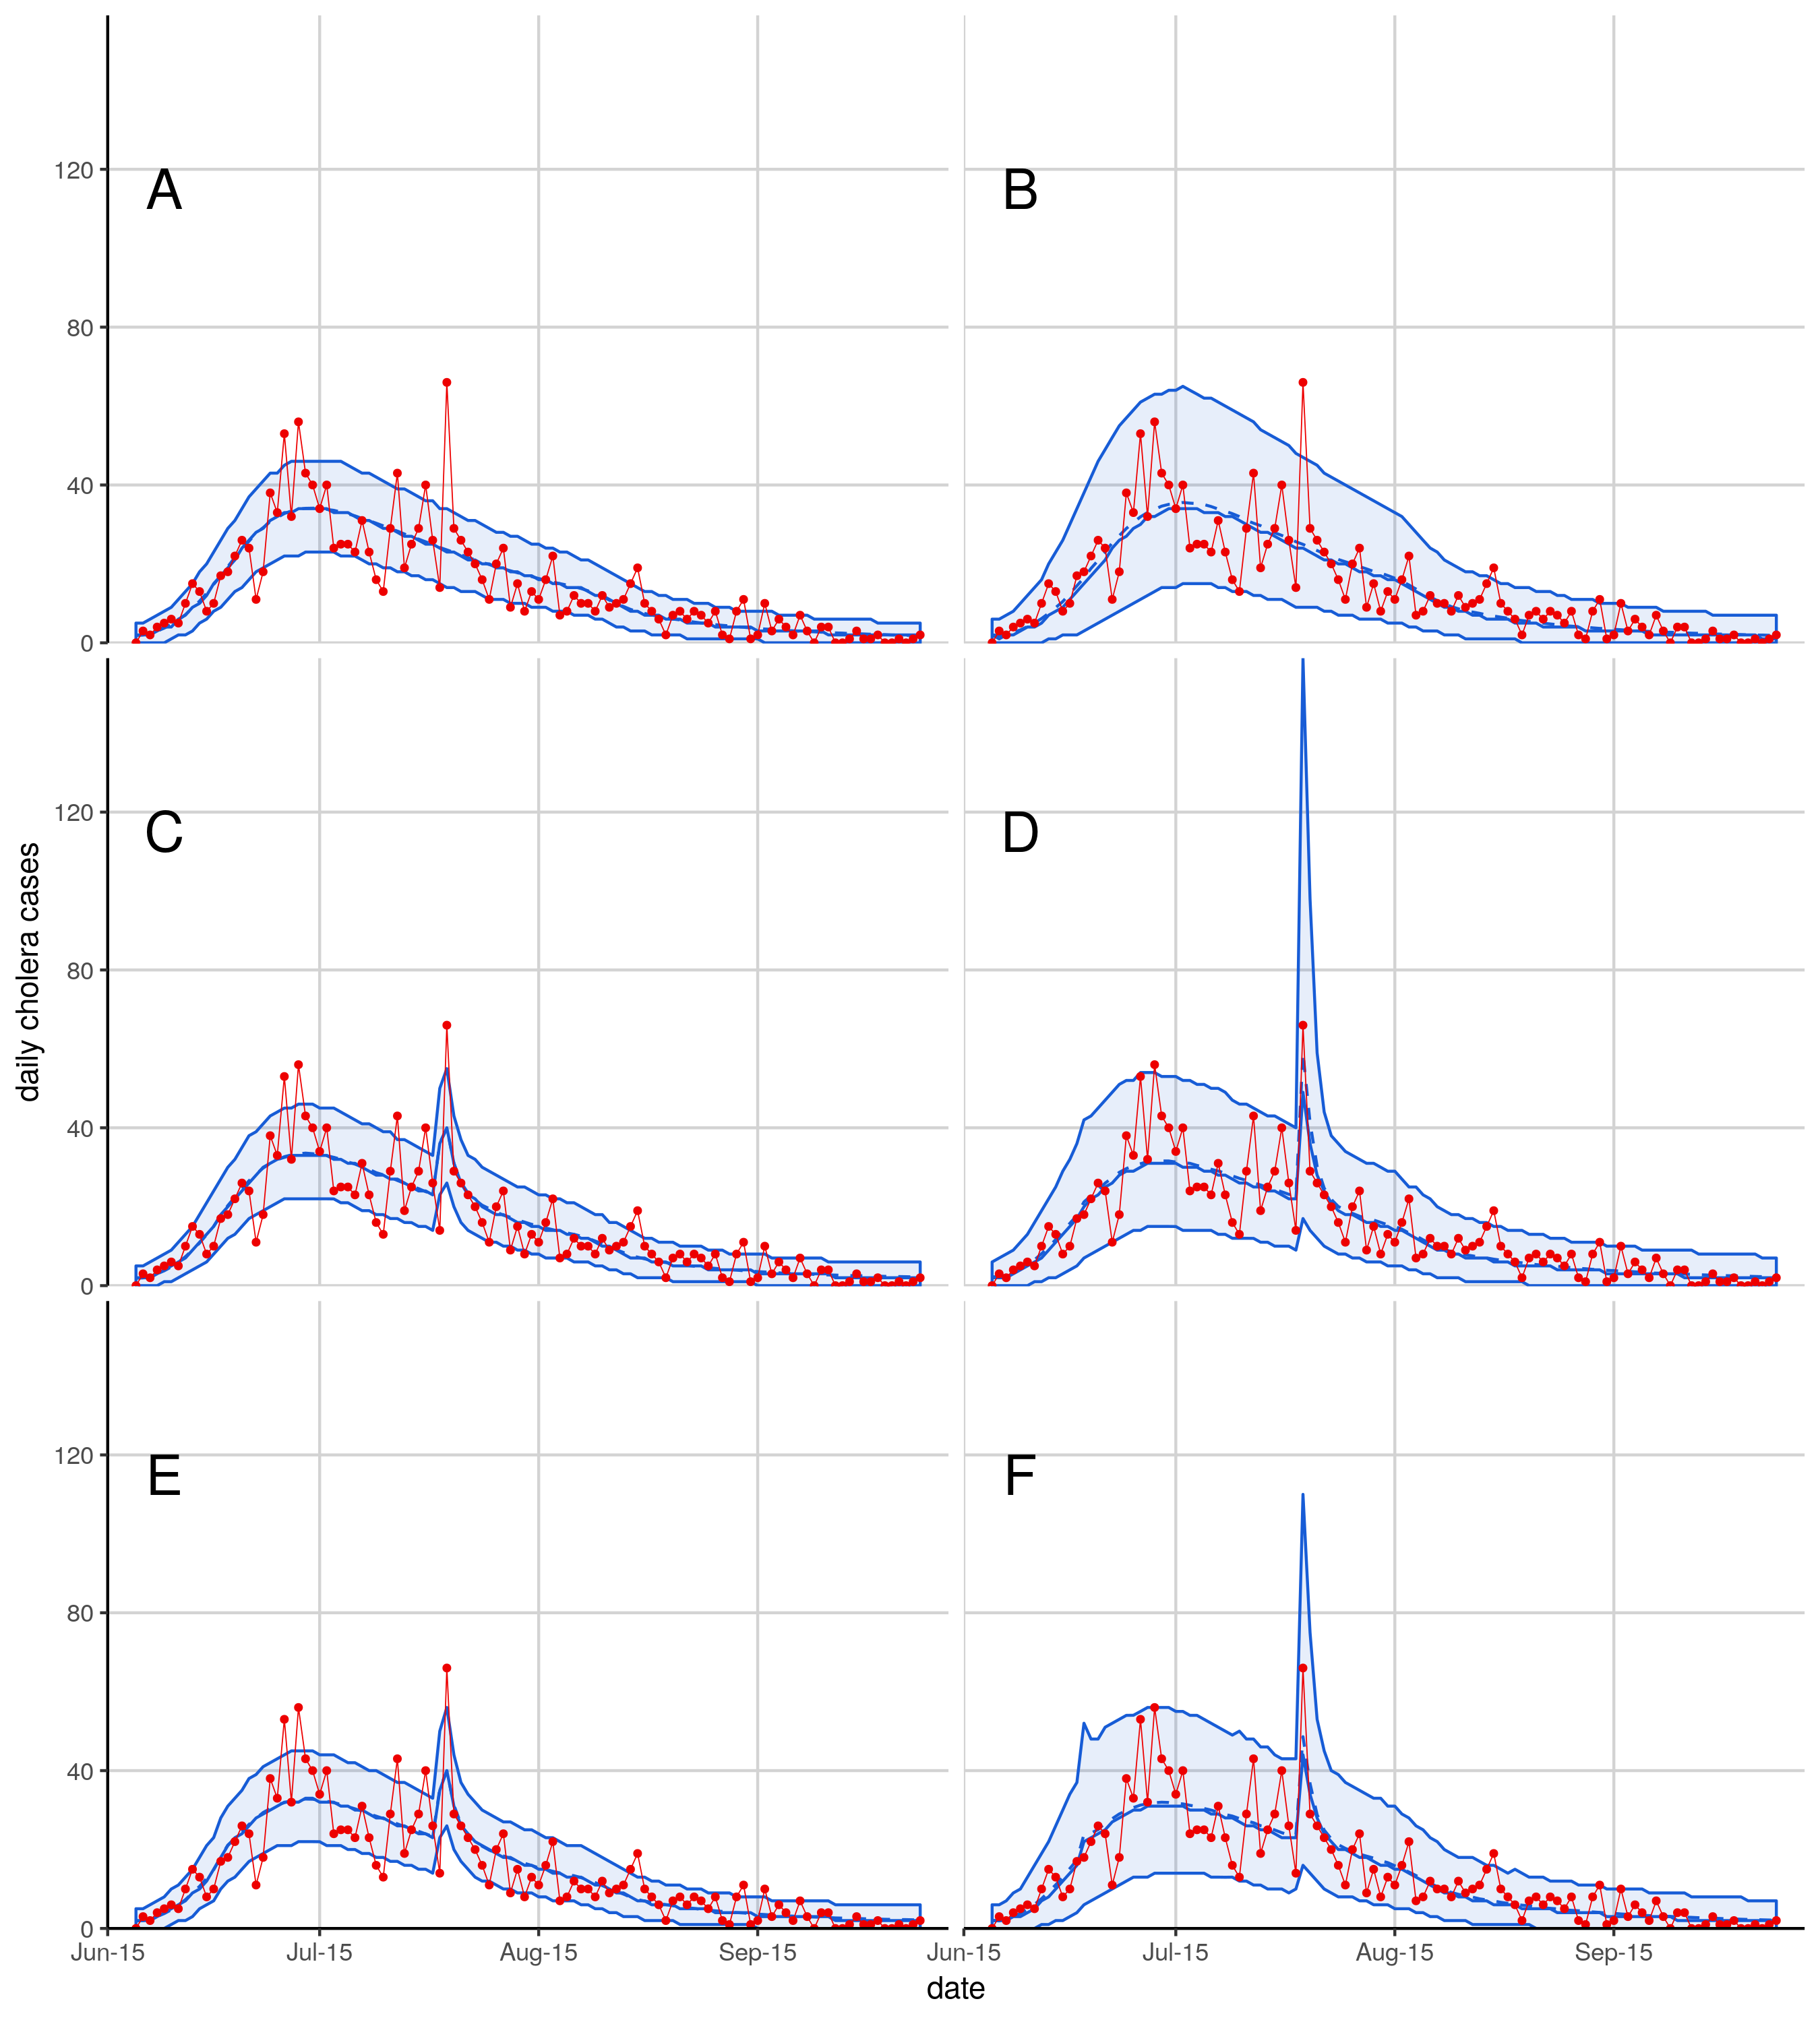
\includegraphics{fig_cholera-rainfall/Lemaitre_ACTROP_2018_42_R1_fig4.png}
    \caption[Fit of the different models]{Simulations of the \textsc{mn} (A-B), \textsc{me} (C-D) and \textsc{mec} (E-F) models. Simulations for the deterministic versions (A,C,E) are given by the mean (blue dashed line), median (blue full line) and 95\% simulation envelops (blue ribbon) of 100 simulations of the measurement model for each trajectory from 100 samples from the posteriors of model parameters against reported daily cholera cases (red line and dots). Simulations from the stochastic models (B, D, F) are given for 10'000 simulations of the stochastic process and measurement models.}
    \label{fig:sim}
\end{figure}

Comparing the two model types, stochastic results have a larger 95\% confidence interval, which better encompass most of the data. In particular, both epidemiological peaks are well captured by the stochastic models, while the deterministic results systematically underestimate them. Two factors contribute to this result: the intrinsic stochastic nature of the model, that requires the simulation of various model runs for the same set of parameters, and the noise that necessarily perturbs the force of the infection yielding an overdispersion in infections. The standard deviation of such (assumed white) noise is estimated in each stochastic model, and it is interesting to note that the MLE obtained for \textsc{ME} is slightly smaller than in \textsc{MN} (0.028 versus 0.022), highlighting again that the data are retrieved with a lower uncertainty when rainfall is included in the model. This is evident in fig.~\ref{fig:sim}, where the width of the 95\% confidence interval of models \textsc{me} and \textsc{mec} is smaller with respect to \textsc{mn}.

Finally, despite having different BFs, the deterministic models \textsc{me} and \textsc{mec} are qualitatively similar in terms of output response, indicating that the recorded changes in the log-likelihood function do not correspond to qualitative changes in the output.

\section{Discussion}
\label{sec:disc}

In this chapter, a general mechanistic SIRB-based epidemiological model is developed to evaluate the relevance of rainfall in the amplification of cholera transmission, focusing on the 2015 Juba outbreak. Two rainfall-based transmission processes were compared: the direct increase of the exposure to the contaminated water (model~\textsc{me})\cite{Eisenberg:ExaminingRainfallCholera:2013}, and the increase of water contamination by flooded open defecation sites (model~\textsc{mc})\cite{Rinaldo:Reassessment20102011:2012}. In addition, human-to-human transmission is considered (models' name with \textsc{H}).

Regarding the epidemiological model, this study introduced two innovations with respect to previous modeling attempts of cholera epidemics\cite{Bertuzzo:ProbabilityExtinctionHaiti:2016,Pasetto:RealtimeProjectionsCholera:2017}. First, the focus on daily incidence data, as opposed to weekly epidemiological reports commonly used in cholera studies, motivated the introduction of a compartment of exposed individuals, eqn.~\eqref{eq:E2j}, to account for the incubation period of the disease and, thus, the lag between the possibly rainfall-driven infection process and the manifestation of the symptoms resulting in the timeseries of daily reported cases at our disposal. %Such compartment had not been considered in previous cholera modelling works because they were most often working with weekly case reports. It was deemed necessary in this study to properly align the daily rainfall forcing with the daily reported cases.
Second, a non-linear version of rainfall driver, in the form of a power-law controlled by a single parameter, was introduced to generalize the previous linear dependence. Such formulation has the flexibility to either emphasize the impact of the largest rainfall events, or give equal weight to all non-zero rainfall intensities. %Suffice here to mention that the added parameter is properly discounted in the formal model comparison carried out here.  
%The idea is that large rainfall events may have a larger role in the deterioration of the sanitation conditions and, thus, in increasing the risk of transmission. The power low used for this goal allows, trough its parameter $\alpha$, to emphasize large precipitation events or to flatten the effect for all precipitation. 

All model assumptions were compared for both deterministic and stochastic model's types, in order to draw more general conclusions. The statistics and tests used to compare the model results  (tab.~\ref{tab:stats} and fig.~\ref{fig:lltests}) supported the significance of rainfall effects during the 2015 epidemic in Juba. In fact, results showed that for both model types there exists a significant positive effect of including rainfall drivers, in particular because standard SIRB models were not able to reproduce the second epidemiological peak of reported cases occurred in July during the recession period. All models considering rainfall, instead, showed an increase of the number of cases in correspondence of the second peak, which was due to the large rainfall rates occurred during the previous days (fig.~\ref{fig:sim}). 
This difference in the simulated responses of models considering (or not) rainfall lead to stronger support for rainfall-based models. Due to the small variations among the likelihoods of rainfall-based models, however, it is not straightforward to draw conclusions on the best way to include the rainfall effect (tab.~\ref{tab:stats}).
Models with the minimum BIC were those considering the increase in exposure (model \textsc{me}) for both the stochastic and the deterministic model types. For the deterministic models, the computation of the Bayes Factors (BFs), which should provide a direct estimation of the model probability, suggested the selection of the model combining exposure and contamination processes (model \textsc{mec}). However, this information criterion might be unstable due to numerical issues and oscillations in the \textsc{mcmc} used for calibration\cite{Raftery:EstimatingIntegratedLikelihood:2007}. By considering the fact that the models' outputs were similar for \textsc{mec} and \textsc{me} (fig. \ref{fig:sim}), it is advised to select the approach endowed with less parameters\footnote{in an attempt to maximize the model predictive accuracy we want to reduce potential overfitting.}, in this case~\textsc{me}, as indicated by the BIC. Note that the inclusion of human-to-human transmission was not statistically relevant in this modeling exercise.

\marginnote{It is also possible that the stochastic model has benefitted from improved indentifiablity. It has been shown that stochastic models can often extract more information about parameters than deterministic counterparts, see: 
\fullcite{Browning:IdentifiabilityAnalysisStochastic:2020}.}
The comparison between the likelihoods of the two models' types (deterministic and stochastic) showed that considering the stochasticity of the processes improves the model results (tab.~\ref{tab:stats}). This suggests that also deterministic models should include a stochastic term in the computation of the force of infection, eqn.~\eqref{eq:force2}, which might increase the flexibility of the outputs.

Several limitations should be considered when analyzing the present results. The calibration exercise attempted in this study considered daily rainfall and cholera reported cases, which are characterized by significant random fluctuations that might partly cloud the description of the underlying infection processes. 
Small random delays in reporting could change the infection curve and thus the effect of rainfall. This issue was partially addressed by considering the exposed compartment, eqn. \eqref{eq:E2j}, for simulation of the incubation period, and unknown reporting rate $\epsilon$ for the observed cases.

Here, it is aimed to reproduce the epidemic by modelling epidemiological transmission processes. %As usual for modelling studies, the level of description of such processes is chosen by balancing model complexity and accuracy: an increase in the number of modelled processes results in a larger number of unknown parameters, and thus a more complex calibration of the model.
While non-linear rainfall effects and possible over-reporting are taken into account, human mobility effect\cite[-4\baselineskip]{Gatto:GeneralizedReproductionNumbers:2012,Bertuzzo:SpatiallyExplicitModels:2010,Mari:PredictiveAbilityMechanistic:2015,Perez-Saez:ClimatedrivenEndemicCholera:2017} is not considered, which could help modeling the importation of infected individual.  Moreover, in this model asymptomatic infected individuals do not contribute transmission. From a modeling viewpoint, these unaccounted processes were compensated by the calibration procedure, at the loss of predictive power.

The prior bounds to be assigned to parameters are typically wide\cite{Akman:ExaminationModelsCholera:2016} because the rates governing transmission processes are highly dependent on the specific epidemiological context, so that somewhat contradictory values had been estimated in literature. These considerations, together with the intrinsic noise affecting recorded cases, underlie the possibility that some of the model parameter might be unidentifiable\cite{Eisenberg:IdentifiabilityEstimationMultiple:2013}, in the sense that different parameter combinations would yield the same model output (also called equifinality). 
The exploration of the posterior parameter distribution using an \textsc{mcmc} approach allowed us to evince the possible correlation among parameters that were well identified by the data, with the main risk of the algorithm getting trapped in a local minimum of the fitness landscape (the distribution of parameters). The posterior probability distributions of the model parameters (see the postprint supplementary information, Section S4) are associated with the model uncertainty, and were here explored by the chains of the \textsc{mcmc} calibration.

The lack of available data prevented us to include the effects of the overall efforts towards WaSH improvement in this study, but vaccination is implemented in order to eliminate one possible covariate of the rainfall effect. 
Despite these limitations, the proposed model comparison using both a deterministic and a stochastic model gave coherent results. The agreement of the two modeling types strengthened the results regarding the importance of rainfall patterns to significantly affect the development of cholera cases in time.

Overall, the findings of the study are consistent with the lessons learned in South Sudan with most of the transmission starting with the onset of the rainy season. In 2016 and 2017, cases in the dry season were observed and associated to the overexploitation of scarce water resources by nomadic herdsmen. This suggests that, as already observed, a general assessment of the relationship between precipitation and general waterborne or water-based disease infections is far from obvious and surely case-dependent. It has been argued, for example, that in the domain of water-based parasitic infections rainfall could not only boost disease transmission but also reduce it substantially\cite[-12\baselineskip]{McCreesh:ChallengesPredictingEffects:2013}, e.g. by increasing water flow (which in turn decreases habitat suitability in water). Rainfall patterns may also drastically affect human activities related to water contacts, thus potentially altering exposure and transmission risk\cite{Lai:SpatialDistributionSchistosomiasis:2015}. To that end, a hydrology-driven assessment cannot ignore certain characteristics, in particular the ephemeral or permanent nature of the waterways fostering contacts among pathogens and hosts\cite{Perez-Saez:HydrologyDensityFeedbacks:2016}. Also, temporal fluctuations of rainfall patterns may be particularly important in determining the seasonality of transmission\cite{Bertuzzo:HydroclimatologyDualpeakAnnual:2012,Bertuzzo:PredictionSpatialEvolution:2011,McCreesh:PredictingEffectsClimate:2015,Perez-Saez:HydrologyDensityFeedbacks:2016}.


%Subsuming the results obtained by this major computational exploration focused on the analysis of Juba's 2015 epidemics, it is concluded that rainfall patterns are fundamental drivers for epidemic cholera models, whether deterministic or stochastic, not only to capture seasonal trends, but also to describe short-term fluctuations in the number of reported cases. 


%\begin{fullwidth}
\chapter[Estimating the probability of eliminating cholera from Haiti through a mass vaccination campaign]{Estimating the probability of \\ eliminating cholera from Haiti \\ through a mass vaccination campaign}%Spatial stochatic model for modeling\\cholera elimination through mass vaccination campaigns}

This chapter describes a model developed for a multi-modelling study. Four teams with existing experience in modeling cholera in Haiti were tasked to model scenarios of mass vaccination administration towards cholera immunity. The timing was meant to take advantage of the low incidence to affect the endemicity of cholera in Haiti in order to achieve elimination. The multi-model study was led by Elizabeth C. Lee and has been published as:

	\longfullcite{Lee:AchievingCoordinatedNational:2020}%\footnote{ECL, ASA, JL, and LCI conceived of the study and contributed to project administration. ECL, DLC, JCL, and LM did the primary modelling analysis, and ECL, DLC, JCL, LM, DP, JP-S, and FF wrote the model supplements. FF, RT, KV, and LCI contributed to data collection. ECL and JL wrote the first draft of the report. ECL, DLC, JCL, LM, DP, JP-S, JDS, FF, MEH, IML, ASA, JL, and LCI contributed to the study design, and all authors contributed to data interpretation and revision of the report.}. 


For this collaborative effort, a hidden Markov model of cholera transmission is developed, with specific modeling choices to account for vaccination and to gather information on elimination timing and probability.
The present chapter is adapted from Supplement 3 of the aforementioned publication, which focuses on the model designed by our team. The reader is referred to the publication by Lee et al. for the modeling exercise results and the comparison between models predictions.
\label{ch:cholera-haiti-ocv}
\end{fullwidth}


\paragraph{Cholera in Haiti} In January 2010, an earthquake hit Haiti, disrupting healthcare and water infrastructure and displacing a million persons. Ten month later, Cholera (\textit{V. Cholerae} of serogroup O1, serotype Ogawa and biotype El Tor) was introduced in Haiti by United Nation peacekeeper soldiers\cite[-3\baselineskip]{Frerichs:NepaleseOriginCholera:2012, Piarroux:UnderstandingCholeraEpidemic:2011}. 
This introduction in a naive population caused a major outbreak, totalling 820'000 reported cases and 10'000 death, most of them occurring in the first two years\cite[-1\baselineskip]{Barzilay:CholeraSurveillanceHaiti:2013}.  Since 2016, cases decreased steadily and finally the last cholera (culture) confirmed case occurred in early 2019\cite{Mitchell:PAHOWHOHaiti:2020}. Cholera exhibited a seasonal pattern with two annual peaks, and spread in every department of the country (fig. \ref{fig:data2}).
\begin{figure*}
	\centering
	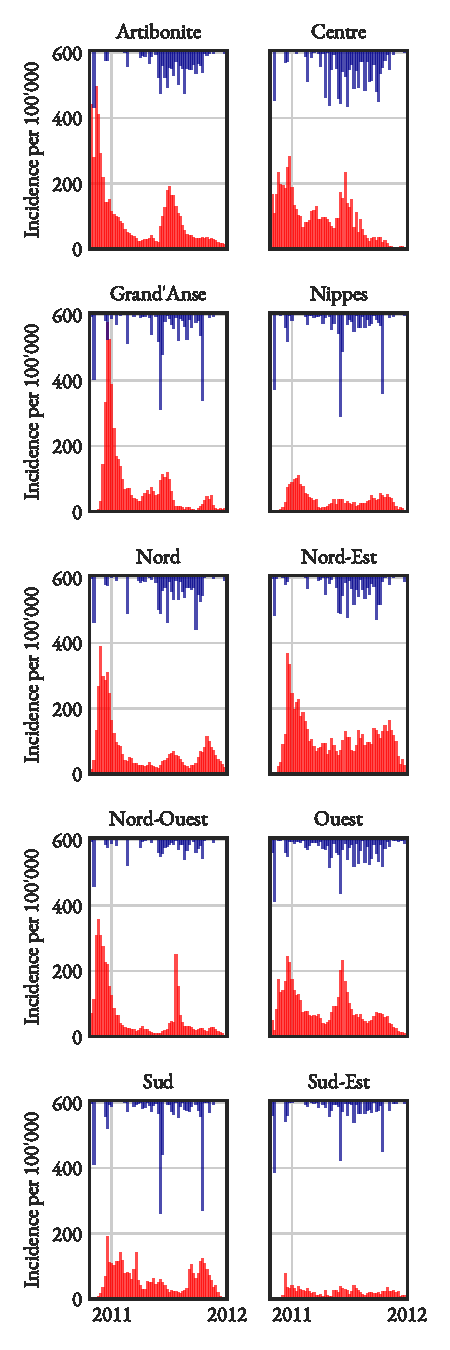
\includegraphics[height=11cm,keepaspectratio]{fig_cholera-haiti-ocv/haiti-2010.pdf}
		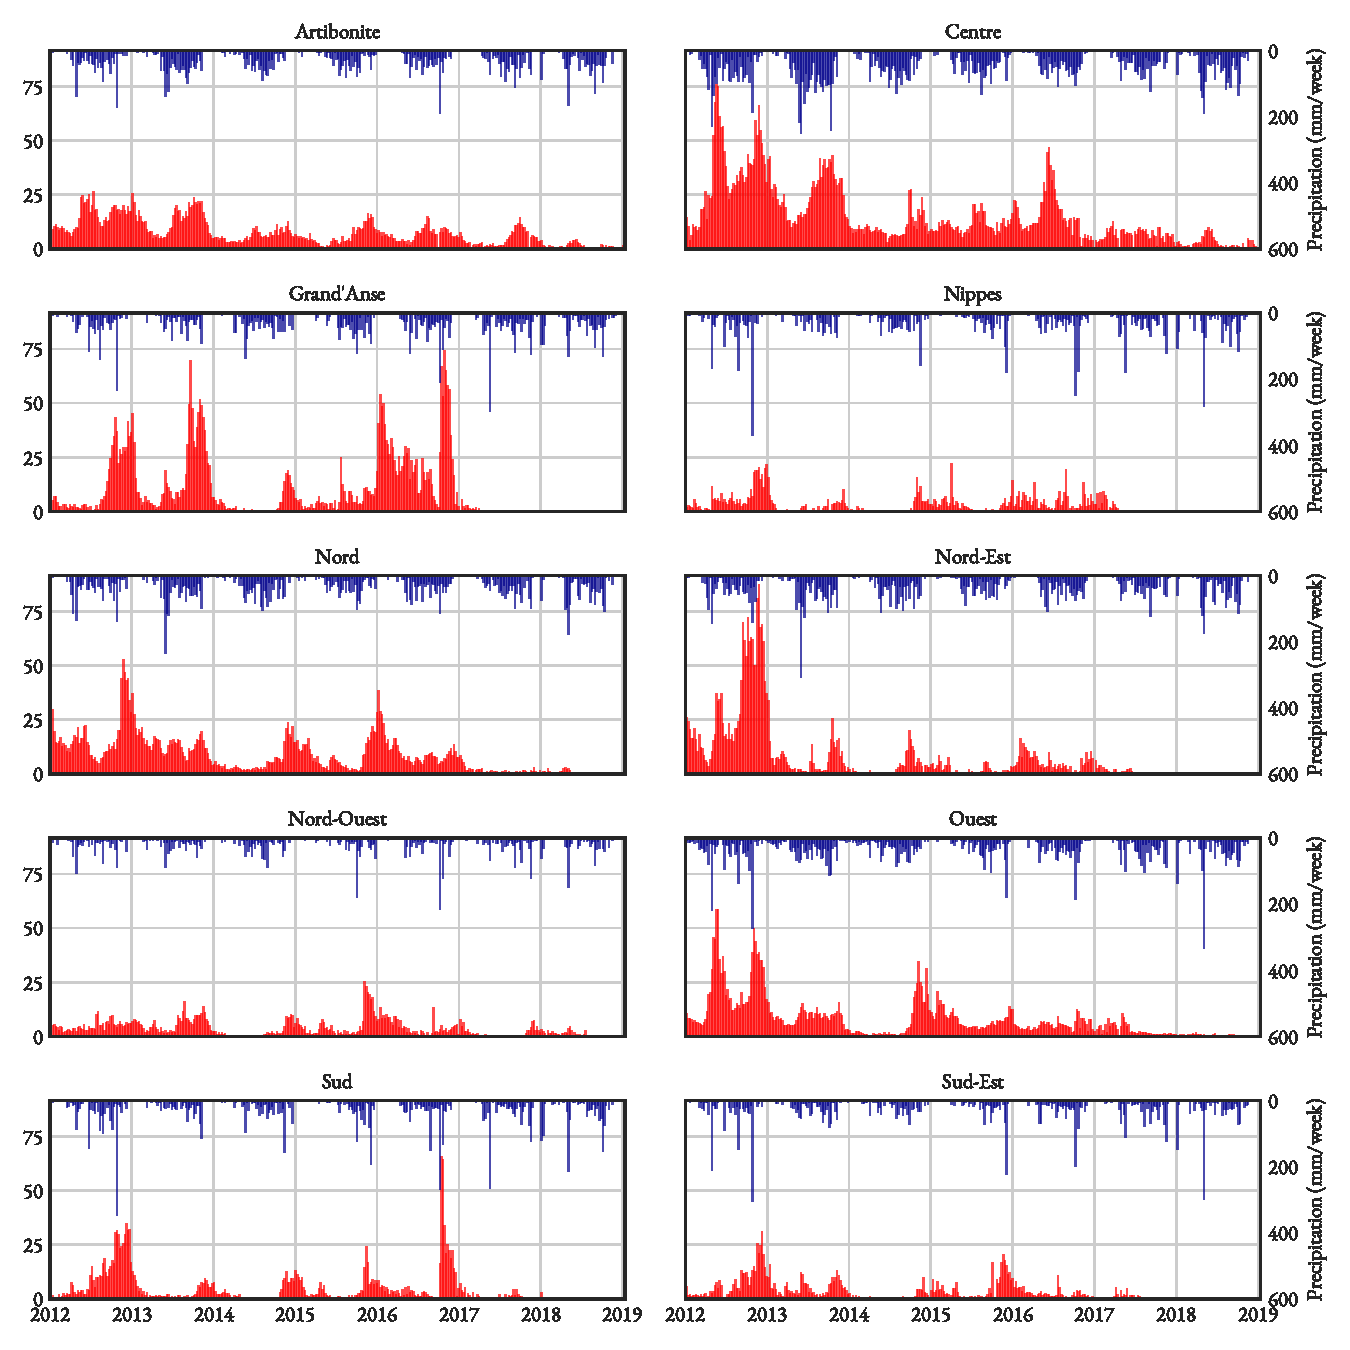
\includegraphics[height=11cm,keepaspectratio]{fig_cholera-haiti-ocv/haiti-2012.pdf}
	\caption[Incident cholera cases and rainfall in Haiti from 2010 to 2019]{Weekly incident cases and rainfall in the ten departments of Haiti from 2010 to 2019. Note that the first two years are shown with a different scale. The ressurgence in 2016 is linked to hurricane Matthew \parencites{Pasetto:RealtimeForecastingCholera:2018,Khan:AssessmentRiskCholera:2017}. The seasonality pattern is evident especially in Artibonite.}
	\label{fig:data2}
\end{figure*}


\section{Description of the model}
% Describe structure of their model and make appropriate references to their previous work. Ideally this will include at least one diagram illustrating the assumed natural history of disease and how vaccination works within the model and appropriate ODE/PDEs

\paragraph{General principles} The cholera model adopted to study the Haitian epidemic is a stochastic compartmental model applied at the level of the ten Haitian departments. 
The model is based on a Partially-Observed Markov Process (POMP), simulating the stochastic transitions between compartments as discrete events. 
It is the stochastic translation of a deterministic SIRB model based on ordinary differential equations which has been extensively used to simulate the Haitian cholera epidemic in previous studies\cite[-8\baselineskip]{Rinaldo:Reassessment20102011:2012,Bertuzzo:ProbabilityExtinctionHaiti:2016,Pasetto:RealtimeForecastingCholera:2018} and is described in \textsc{Chapter~1}. % ,Camacho:PredictionCholeraDynamics:2016
The model subdivides the population of each department\footnote[][9\baselineskip]{The case data was provided for the ten departments of Haiti, so the model spatial unit was choosen to be the department. Other teams decided either the same scale, coarser (national for Lee et al.) or finer (1km grid for Chao et al.).} into compartments counting the number of individuals at the different stages of the disease. In addition to susceptible $S$, symptomatic infected $I$ and recovered individuals $R$, a compartment for infectious asymptomatic $A$ is added for the purpose of this exercise. As in previous chapters,an environmental compartment describing the bacterial concentration $B$ in the local environment is used to estimate the force of infection. Precipitation is an important environmental driver of cholera transmission\cite{Camacho:CholeraEpidemicYemen:2018}, especially in Haiti\shortcite{Rinaldo:Reassessment20102011:2012}. As done in the contamination formulation in \textsc{Chapter~2}, rainfall increases the rate at which bacteria shed by infected individuals enter the environmental reservoir and thus increases the bacterial concentration and finally the force of infection. A diagram of the model is given in fig.~\ref{figEPFL}.
\subsection{Model dynamics} 
The following cholera dynamics are included in the model:
\begin{description}
    \item[Force of Infection and mobility] The force of infection in each department contains as additional term  the number of cholera cases in the rest of Haiti. This allows for a possible introduction of cholera due to  human mobility between departments. The force of infection in each department is composed of two parts. The first is related to the local bacterial concentration of the department. The second is related to case importation from other departments through human-to-human transmission. The corresponding equation for the $i^{th}$ department reads:
    \marginnote[-5\baselineskip]{The force of infection uses indirect (water-mediated) local transmission but direct (human-to-human) transmission for mobility exchanges. One of the reasons behind this discrepancy is technical: scalability issues linked to particle depletion hinder iterated filtering performance. Thus, it becomes very hard to calibrate a spatial model. To alleviate this issue, a custom procedure has been developed (see below) that was only tractable with simple mobility link. Instead today, the choice would be to use the improved methods that have been developed for spatial inference on pomp models \parencite{Asfaw:PartiallyObservedMarkov:2021, Park:InferenceHighdimensionalImplicit:2020}.}
    \begin{equation*}
    F^i_0(t)=\beta^i\frac{B_i(t)}{1+B_i(t)}+c^i \sum_{j\ne i} (I_j(t)+A_j(t)).
    \end{equation*}
    The first term in the sum represents local transmission governed by the department-specific exposure parameter $\beta^i$ which multiplies the logistic dose-response of the re-scaled local bacterial concentration $B = B^*/K$, where $B^*$ is the unscaled concentration of vibrios and $K$ the half-saturation constant of the logistic function $\frac{B^*_i(t)}{K+B^*_i(t)}$.
    Case importation from other departments is given by the sum of the asymptomatically and symptomatically infected in department $j$, modulated by a parameter $c^i$ which represents the intensity of case introduction from other departments in Haiti  to department $i$.
    \item[Rainfall] We account for rainfall using the contamination pathway described in the previous chapters. Rainfall increases the amount of \textit{Vibrios} per infected individual that contaminate the water reservoir. In Haiti, rainfall was empirically associated with resurgence of cholera infections in many research works\shortcite{Gaudart:SpatioTemporalDynamicsCholera:2013,Bertuzzo:ProbabilityExtinctionHaiti:2016,Adams:HaitiPreparesCholera:2012,Periago:EliminationCholeraTransmission:2012,Adams:CholeraHaitiTakes:2013,Rinaldo:Reassessment20102011:2012,Eisenberg:ExaminingRainfallCholera:2013,Kirpich:CholeraTransmissionOuest:2015}
    \item[Symptoms] A proportion $\sigma$ of infected individuals become symptomatic, and $1-\sigma$ remain (shedding, hence infectious) asymptomatic and transitions into compartment $A$ (instead of $R$ in previous chapter, because past model formulation did not account for shedding asymptomatic).
    \item[Shedding] Both symptomatic and asymptomatic infected individuals shed bacteria. The shedding rate of asymtomatics, $\theta_A$, is modeled as a fraction of the shedding rate of symptomatic individuals  $\theta_I$\cite{Kuhn:GlucoseNotRiceBased:2014}.
    \item[Recovery rate] The recovery rate is the same for both asymptomatic and symptomatic individuals ($\gamma_I=\gamma_A=0.2$ d$^{-1}$)\cite{Kaper:Cholera:1995, Codeco:EndemicEpidemicDynamics:2001}.
    \item[Acquired immunity] Individuals acquire natural immunity and remain in the recovered compartment ($R$) for a period that lasts for $1/\rho=$ 8 years on average, before reintegrating the susceptible compartment\footnote{This was surprisingly consistent across teams, with values ranging from 5 to 8 years.}.
    \item[Erlang-distributed immunity loss] To model extinction through coordinated immunity, it is needed to better approximate distribution that typically characterizes the duration of immunity\cite{King:InapparentInfectionsCholera:2008}. Instead of a exponential distribution, recovered individuals pass through a succession of three separate recovered compartments ($R_1$, $R_2$, $R_3$) characterized by the same transition rate $\rho_1=\rho_2=\rho_3=3\rho$. Hence the duration of immunity is Erlang-distributed.
    \item[Bacterial dynamics] The size of the bacterial reservoir is proportional to the population density $D_i$ of the department. This is another difference with respect to past models which used population. The goal is better capture the risk posed by cholera in slums and dense urban areas such as Port-au-Prince. Bacteria die at rate $\mu_B$ (with a mean persistence, calibrated, of less than three days). Rainfall influences the bacteria concentration by increasing the rate at which bacteria enter the environmental reservoir.
    \item[Reporting process] The reported cases are modelled by a negative-binomial distribution with dispersion parameter $p$. Over- or under-reporting is accounted for through the reporting parameter $\epsilon$.
\end{description}
    
    
\paragraph{Stochasticity} Overdispersion in the infection process is introduced by multiplying the force of infection $F_0$ by a time-continuous white noise process \(\xi(t)\) defined as the differentiation of an integrated noise process \(\xi(t) = \frac{d}{dt}\Gamma(t)\), here taken to be have a Gamma distribution with mean \(\Delta t\) and variance \(\sigma^2 \Delta t\)\cite[-3\baselineskip]{Breto:CompoundMarkovCounting:2011}:

\[
\xi(t) = \Gamma (t+\Delta t) - \Gamma (t) \sim \text{Gamma}\left( \frac{\Delta t}{\sigma^2}, \sigma^2\right).
\]

Since \(\xi(t)\) is non-negative it can serve as a multiplicative noise on
the force of infection: \[
F_i(t) = F^i_0(t) \xi(t),
\]
which yields to over-dispersion in the transitions.
%\(\Delta N_{SE}(t), \Delta N_{SR}(t), \Delta N_{V^SV^E}(t), and \Delta N_{V^SV^R}(t)\).

\begin{figure}%[htbp]
\begin{center}
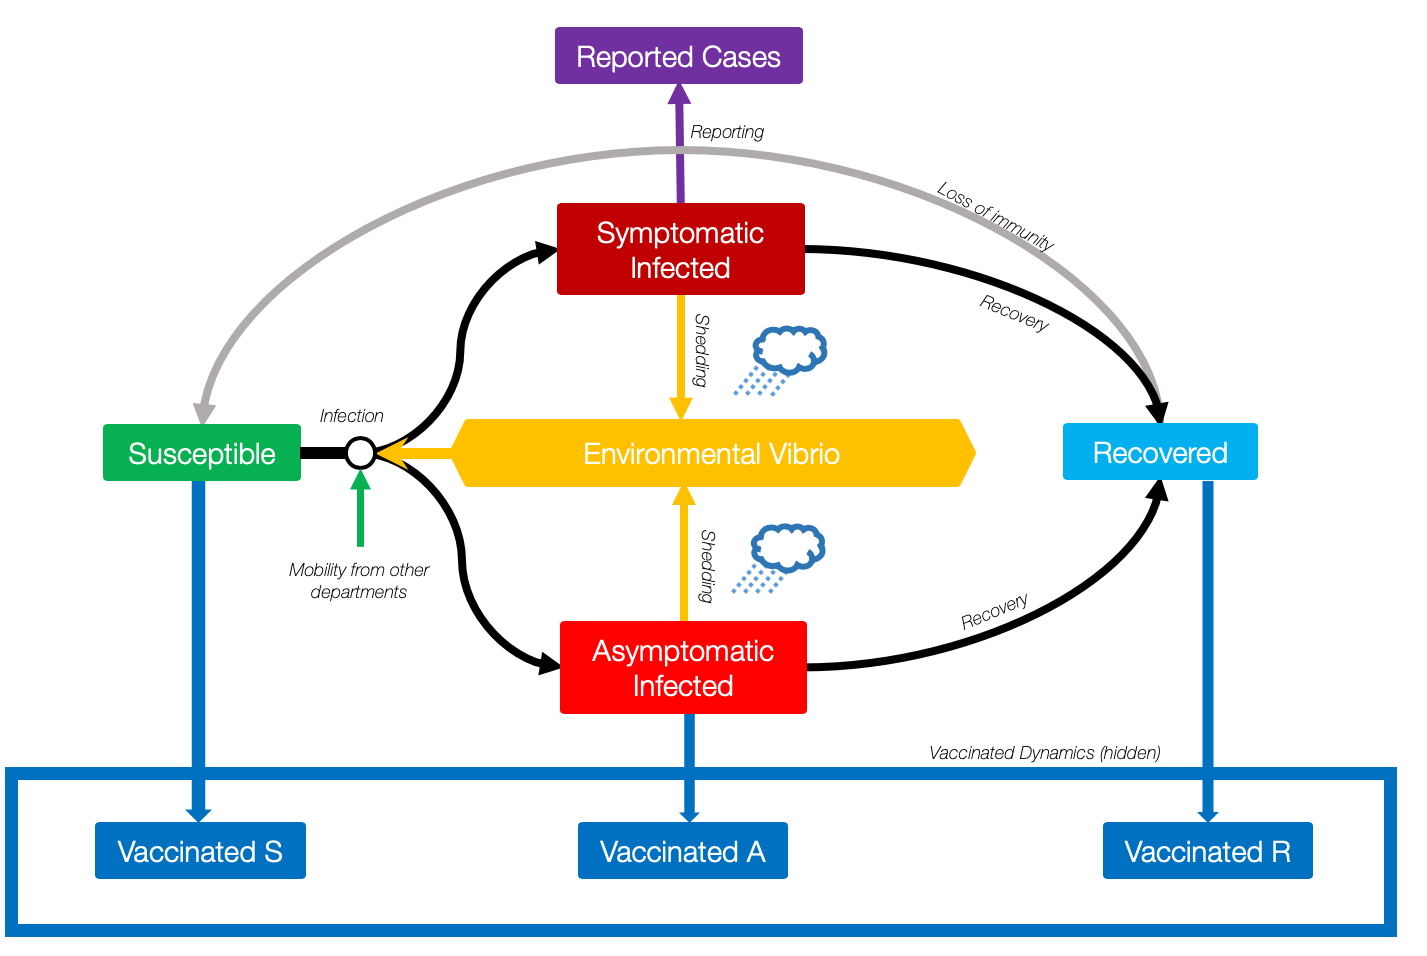
\includegraphics{fig_cholera-haiti-ocv/compartiments.png}
\caption[Schematic diagram of the cholera transmission processes in a single department]{Schematic diagram of the cholera transmission processes in a single department. Dynamics of vaccinated compartments are not shown.}
\label{figEPFL}
\end{center}
\end{figure}

\paragraph{Vaccination dynamics} The estimated vaccine efficacy was waning from 76\% over 60 month for adults, and conservatively assumed to provide no protection after 5 years. These assumptions were shared across modeling teams. 
At each vaccination campaign, the available vaccine doses are uniformly distributed among susceptible $S$, asymptomatic infected $A$ and recovered $R_{1}$, $R_2$, $R_3$ individuals. The rate of vaccination is denoted with $r_V$. Individuals can receive either one or two doses of OCV, which yield efficacies of $\eta_{1d}(t)$ and $\eta_{2d}(t)$, respectively. These parameters are common across modeling teams and the reader is reffered to the manuscript for their time-varying values. There is no age structure but the efficacy is set to be the population-weighted average of estimated efficacy for those under 5 years old and those over 5 years old.
 The model considers ten additional compartments for each vaccination campaign, in order to distinguish among individuals who received one (compartments $V^S_{1d}$, $V^A_{1d}$, $V^{R_k}_{1d}$, $k=$1, 2, 3) or two (compartments $V^S_{2d}$, $V^A_{2d}$, $V^{R_k}_{2d}$, $k=$1, 2, 3) doses of OCV. Vaccinated susceptible individuals ($V^S_{1d}$ and $V^S_{2d}$) have a lower probability to become infected (and thus entering classes $I$ or $A$) than non-vaccinated susceptibles. This is modeled through the multiplicative reduction of the force of infection by a  factor $(1-\eta_{1d}(t))$ or $(1-\eta_{2d}(t))$ respectively.
The vaccination campaign window is split equally between departments (i.e for a vaccination campaign of 5 years duration, each department will be vaccinated during a 6 month period). Vaccine efficacy starts waning after the first half of the duration of the department's vaccination campaign. For example, if for department $i$ the vaccination campaign $j$ spans from $t^{i,j}_a$ to $t^{i,j}_b$, then:
    \begin{equation}
\eta^{i,j}(t) = \left\{
    \begin{array}{ll}
        \eta_0(0) & \mbox{if t $<  t^{i,j}_a + \frac{t^{i,j}_b - t^{i,j}_a}{2}$} \\
        \eta_0(t -  (t^{i,j}_a +  \frac{t^{i,j}_b - t^{i,j}_a}{2}) ) & \mbox{if t $>  t^{i,j}_a + \frac{t^{i,j}_b - t^{i,j}_a}{2}$} \\
    \end{array}
\right.
\end{equation}
where $\eta_0(t)$ is the scenario dependant vaccine efficacy as defined in the meta-supplement.
The rates at which individuals leave compartments $V^A$ and $V^{R_k}$ ($k=$1, 2, 3) are equivalent to $A$ and $R_i$. Individuals enter the compartment $V^S$ with a vaccine efficacy reduced according to the amount of time they spent in $V^A$ and $V^{R_k}$. The actual deployment of the vaccine doses in shown in fig.~\ref{fig:deploy}.

\paragraph{Other interventions} WaSH and other intervention efforts are not explicitly considered in the model, but their impact is implicitly taken into account by calibrating the exposure rates $\beta^i$ to disease incidence that occurred while interventions were taking place. $\beta^i$ is modelled to be constant in time, meaning that changes in number or type of interventions or population behaviour over time are not taken into account. %The goal is to see if elimination is possible independently of WaSH improvement. for discussion


\subsection{Model equations}\label{sec:stoch}
The model is implemented as a stochastic counting process\cite{Breto:TimeSeriesAnalysis:2009}. Let \(N_{AB}(t)\) be the number of individuals transiting between compartments \(A,B\in \mathcal{X}\) in the time interval \([0,t)\)  where $\mathcal{X}$ is the state vector,
$$\mathcal{X} = \{S, I, A, R_k, V^S_{j,1d},V^A_{j,1d}, V^{R_k}_{j,1d}, V^S_{j,2d},V^A_{j,2d}, V^{R_k}_{j,2d}\} 
\text{ for } j = 1, ..., J, \text{ and } k = 1, 2, 3,
$$
%\marginnote{The model formalism is similar to the one used for the stochastic model in \textsc{Chapter~2} and detailled in the \textsc{Appendix}, eqn. \eqref{eq:stochsys}.}
and $J$ is the number of vaccination campaigns in the department.
The number of transitions during a time-step $\Delta t$ is
\(\Delta N_{AB}(t) = N_{AB}(t+\Delta t) - N_{AB}(t)\). Given the state of the system at time \(t\), \(\mathcal{X}_t\), and a force of infection $F_j(t)$ the transition rates read (transitions are written only for one dose of OCV and one vaccination campaign to shorten the equations):
\begin{fullwidth}
\begingroup
\allowdisplaybreaks
\label{eq:stochsys}
\begin{align}
    \mathbb{P}\left[ \Delta N_{SI}(t) = 1 \mid\mathcal{X}_t\right] &= \sigma F_j(t) S(t) \Delta t + o(\Delta t)\\ \label{eq:stochstart}
    \mathbb{P}\left[ \Delta N_{SA}(t) = 1 \mid\mathcal{X}_t\right] &= (1-\sigma) F_j(t) S(t) \Delta t + o(\Delta t)\\
    \mathbb{P}\left[ \Delta N_{SV_{1d}^S}(t) = 1 \mid\mathcal{X}_t\right] &= r_{V_{1d}}(t) S(t) \Delta t + o(\Delta t)\\
    \mathbb{P}\left[ \Delta N_{S\bullet}(t) = 1 \mid\mathcal{X}_t\right] &= \mu  S(t) \Delta t + o(\Delta t)\\
    \mathbb{P}\left[ \Delta N_{IR_1}(t) = 1 \mid\mathcal{X}_t\right] &= \gamma I(t) \Delta t + o(\Delta t)\\
    \mathbb{P}\left[ \Delta N_{I\bullet}(t) = 1 \mid\mathcal{X}_t\right] &= (\mu+\alpha)I(t) \Delta t + o(\Delta t)\\
    \mathbb{P}\left[ \Delta N_{AR_1}(t) = 1 \mid\mathcal{X}_t\right] &= \gamma A(t) \Delta t + o(\Delta t)\\
      \mathbb{P}\left[ \Delta N_{AV_{1d}^A}(t) = 1 \mid\mathcal{X}_t\right] &= r_{V_{1d}}(t) A(t) \Delta t + o(\Delta t)\\
      \mathbb{P}\left[ \Delta N_{A\bullet}(t) = 1 \mid\mathcal{X}_t\right] &= \mu  A(t) \Delta t + o(\Delta t)\\
    \mathbb{P}\left[ \Delta N_{R_kR_{k+1}}(t) = 1 \mid\mathcal{X}_t\right] &= 3\rho R_k(t) \Delta t + o(\Delta t),\quad k=1,2\\
    \mathbb{P}\left[ \Delta N_{R_3S}(t) = 1 \mid\mathcal{X}_t\right] &= 3\rho R_3(t) \Delta t + o(\Delta t)\\
    \mathbb{P}\left[ \Delta N_{R_kV_{1d}^{R_k}}(t) = 1 \mid\mathcal{X}_t\right] &= r_{V_{1d}}(t) R_k(t) \Delta t + o(\Delta t)\quad k=1,2,3\\
    \mathbb{P}\left[ \Delta N_{R_k\bullet}(t) = 1 \mid\mathcal{X}_t\right] &= \mu  R_k(t) \Delta t + o(\Delta t)\quad k=1,2,3\\
    \mathbb{P}\left[ \Delta N_{V_{1d}^SI}(t) = 1 \mid\mathcal{X}_t\right] &=  \sigma (1-\eta_{1d}^{i,j}(t)) F_j(t) V_{1d}^S(t) \Delta t + o(\Delta t)\\
    \mathbb{P}\left[ \Delta N_{V_{1d}^SA}(t) = 1 \mid\mathcal{X}_t\right] &=  (1-\sigma) (1-\eta_{1d}^{i,j}(t)) F_j(t) V_{1d}^S(t) \Delta t + o(\Delta t)\\
    \mathbb{P}\left[ \Delta N_{V_{1d}^S\bullet}(t) = 1 \mid\mathcal{X}_t\right] &= \mu  V_{1d}^S(t) \Delta t + o(\Delta t)\\
    \mathbb{P}\left[ \Delta N_{V_{1d}^AV_{1d}^{R_1}}(t) = 1 \mid\mathcal{X}_t\right] &= \gamma V_{1d}^A(t) \Delta t + o(\Delta t)\\
    \mathbb{P}\left[ \Delta N_{V_{1d}^A\bullet}(t) = 1 \mid\mathcal{X}_t\right] &= \mu  V_{1d}^A(t) \Delta t + o(\Delta t)\\
    \mathbb{P}\left[ \Delta N_{V^{R_k}V^{R_{k+1}}}(t) = 1 \mid\mathcal{X}_t\right] &= 3\rho V^{R_k}(t) \Delta t + o(\Delta t),\quad k=1,2\\
    \mathbb{P}\left[ \Delta N_{V_{1d}^{R_3}V_{1d}^S}(t) = 1 \mid\mathcal{X}_t\right] &= 3\rho V_{1d}^{R_3}(t) \Delta t + o(\Delta t)\\
    \mathbb{P}\left[ \Delta N_{V^{R_k}\bullet}(t) = 1 \mid\mathcal{X}_t\right] &= \mu  V^{R_k}(t) \Delta t + o(\Delta t)\quad k=1,2,3 \label{eq:stochend}
\end{align}
\endgroup
\end{fullwidth}
assuming that \(\mathbb{P}[\Delta N_{XY} > 1\mid\mathcal{X}_t] = o(\Delta t) \; \forall X,Y \in \mathcal{X}\) and \(\mathbb{P}[\Delta N_{X\bullet} > 1\mid\mathcal{X}_t] = o(\Delta t) \; \forall X \in \mathcal{X}\). Note that \(\mathbb{P}\left[ \Delta N_{X\bullet}(t) = 1 \mid\mathcal{X}_t\right]\) denotes probability that individuals die and it is governed by the same parameter $\mu$ for all compartments except $I$. 

The ensuing stochastic variations of the state variables are:
\begin{fullwidth}
\begingroup
\allowdisplaybreaks
\label{eq:stochstates}
\begin{align}
    \Delta I(t) &= \Delta N_{SI}(t) -  \Delta N_{IR_1}(t) -  \Delta N_{I\bullet}(t)\\
    \Delta A(t) &= \Delta N_{SA}(t) -  \Delta N_{AR_1}(t) -  \Delta N_{AV^A}(t) - \Delta N_{A\bullet}(t)\\
    \Delta R_1(t) &= \Delta N_{IR_1}(t) + \Delta N_{AR_1}(t) -  \Delta N_{R_1 R_2}(t) -  \Delta N_{R_1V^{R_1}}(t) -  \Delta N_{R_1\bullet}(t)\\
    \Delta R_2(t) &= \Delta N_{R_1R_2}(t) - \Delta N_{R_2 R_3}(t) -  \Delta N_{R_2V^{R_2}}(t) -  \Delta N_{R_2\bullet}(t)\\
    \Delta R_3(t) &= \Delta N_{R_2R_3}(t) - \Delta N_{R_3 S}(t) -  \Delta N_{R_3V^{R_3}}(t) -  \Delta N_{R_3\bullet}(t)\\
    \Delta V^S(t) &= \Delta N_{SV^S}(t) -  \Delta N_{V^S I}(t)-  \Delta N_{V^S A}(t) - \Delta N_{V^S\bullet}(t)\\
    \Delta V^A(t) &= \Delta N_{AV^A}(t) -  \Delta N_{V^AV^{R_1}}(t) - \Delta N_{V^A\bullet}(t)\\
    \Delta V^{R_1}(t) &= \Delta N_{R_1V^{R_1}}(t) +  \Delta N_{V^AV^{R_1}}(t) - \Delta N_{V^{R_1}V^{R_2}}(t) - \Delta N_{V^{R_1}\bullet}(t)\\
    \Delta V^{R_2}(t) &=\Delta N_{R_2V^{R_2}}(t)+\Delta N_{V^{R_1} V^{R_2}}(t) -  \Delta N_{V^{R_2}V^{R_3}}(t) -  \Delta N_{R_2\bullet}(t)\\
    \Delta V^{R_3}(t) &= \Delta N_{R_3V^{R_3}}(t)+\Delta N_{V^{R_2}V^{R_3}}(t) - \Delta N_{V^{R_3}V^ S}(t) - \Delta N_{V^{R_3}\bullet}(t)\\
    S(t) &= H_i - \sum_{X \in \mathcal{X} \backslash \{S\}} X(t),
\end{align}
\endgroup
\end{fullwidth}
where the equation for $S(t)$ enforces a constant total population. 
The rescaled bacterial concentration $B$ is necessary to estimate the force of infection and is computed using the following ODE:
\begin{equation}
\frac{dB}{dt} = - \mu_B B +  \left(1 + \lambda\left( J(t)\right)^{r} \right)  D_i \left[\theta_I I + \theta_A A\right] 
\end{equation}
where $J(t)$ is the precipitation over time and $D_i$ is the average population density of the department\footnote{total department population over department area. It is assumed that density is more important than population size, a change from the historical model described in \textsc{Chapter~1}}.  Parameter $\mu_B$ expresses the mortality rate of the bacteria in the environment, $\theta_I$ and $\theta_A$ are the shedding rates of symptomatic and asymptomatic infected individuals, and $\lambda$ and $r$ are the parameters of the power-law that controls the non-linear impact of precipitation, as in \textsc{Chapter~2}. The model was simulated with a constant time-step of $4.8$h, and the ODE for the bacterial concentration was integrated using a Runge-Kutta 4 scheme.



Let \(C(t_j)\) denote the number of people that develop symptoms and seek healthcare during the
observation interval \([t_j, t_{j+1})\) (i.e. the true incidence). Thus:

\begin{equation}
    C(t_j) = [N_{SI}(t_{j+1}) - N_{SI}(t_j)] + [N_{V^SI}(t_{j+1}) - N_{V^SI}(t_j)].
\end{equation}

Our Markov process formulation requires a measurement model linking the time series of the reported incidence to \(C(t_j)\) as the observed variable to the process model in eqn. \eqref{eq:stochsys} . A negative-binomial measurement model accounting for over- or under-reporting of cholera incidence os choosen, i.e.
\[
	\text{cases}(t_j) \sim \text{NB}(\epsilon(t) C(t_j), p).
\]
where \(\epsilon(t) > 0\) represents the proportion of cases reported. To account for the change of the case definition that occurred on January 1, 2018, the reporting rate changes over time:
\begin{equation}
\epsilon(t) = \left\{
    \begin{array}{ll}
        \epsilon_1 & \mbox{if t $<$ Jan 1st, 2018} \\
        \epsilon_2 & \mbox{otherwise}
    \end{array}
\right.
\end{equation}

The parameters of the model are shown in tab.~\ref{paramEPFL}.



% Table with all model parameters indicating whether each is fit or assumed (with some description of assumptions) and appropriate references to primary literature (please don't cite previous parameters used in modeling studies).

\begin{table*}
\caption{Model parameters%References:%\fullciteshortb{Levine:DurationInfectionDerivedImmunity:1981, Koelle:DisentanglingExtrinsicIntrinsic:2004, Bertuzzo:SpacetimeEvolutionCholera:2008, Kaper:Cholera:1995}
}
\begin{tabular}{lcccl}
\toprule
Parameter & Calibration & Value or bound & Unit & description \\
\midrule
$\beta^i$ ($\times 10$ dept.) & yes & $[0,\infty]$ & -- & Exposure  \\
$c^i$ ($\times 10$ dept.) & yes & $[0,\infty]$& -- & Force of infection in dept. $i$ from cases in other depts. \\
$\epsilon_1$& yes & $[0,2]$ & --& reporting fraction before January 1, 2018\\
$\epsilon_2$& yes & $[0,2]$ & --& reporting fraction after January 1, 2018\\
$\sigma_w$ & yes& $[0,0.1]$ & --&  std-dev of the perturbation of $F(t)$\\
$p$& yes &$[0,\infty]$ & --&  dispersion parameter of reporting\\
$\theta_I$  & yes &   $[0,\infty]$ & --& Shedding sympt.  \\
$\theta_A$  & yes &  $[0,\theta_I]$ &  --& Shedding asympt. \\ 
$\mu_B$   & yes & $[0,\infty]$ &d$^{-1}$ & Bacterial mortality in environment \\ 
$r$       & yes &  $[0,\infty]$ & --& Exponent rainfall \\ 
$\lambda$  & yes &   $[0,\infty]$ & --& Coef. rainfall \\ 
$\rho$  & no & $1/(8\cdot365)$ &d$^{-1}$ & Loss of immunity (Levine et al.,1981 and Koelle et al, 2004)\\ 
$\sigma$  & no & $0.25$ & -- & Symptomatic/exposed \\  
$\alpha$  & no &  $0.004$ & d$^{-1}$& Mortality due to cholera (Bertuzzo et al., 2008)\\ %estimated based on data in Enrico's paper
$\gamma$  & no & $1/5$& d$^{-1}$ & Recovery rate  sympt. (Kaper, 1995)\\  
$k$    & no  & $3$ & --& number of recovered compartments \\
$\mu$  & no &  $1/(63.6\cdot365)$ &d$^{-1}$ & mortality rate from life expectancy (World bank, 2017)\\  
$\eta_{1d}(t), \eta_{2d}(t)$ & no  & as in spec. & --& Vaccine efficacy for 1 and 2 doses \\
\bottomrule
\end{tabular}
\label{paramEPFL}
\end{table*}

\section{Calibration of the model}
% Description of additional data
\paragraph{Data} Remote-sensed precipitation estimates from NASA's TRMM and GPM missions are used\footnote{TRMM 3B42 RT Derived Daily Product \parencite{Huffman:TRMMMultisatellitePrecipitation:2007} is used from October 2010 to March 2015,  and GPM from from April 2015 to December 2019.}. Rainfall measurements are provided on a regular grid. To get a value for each department, the measurements are averaged over the extent of the department. The time series of future rainfall up to the year 2030 is constructed by sampling from the past 20 years of data  with replacement blocks of 15 days. To keep the correct seasonality the day of the year of each block is preserved.

\paragraph{Fitting procedure} The model is calibrated separately for each department on the weekly reported cases from March 1, 2014 to January 1st 2019. The calibration procedure is based on a frequentist multiple iterated filtering algorithm (MIF2)\cite{Ionides:InferenceDynamicLatent:2015}. The initial conditions on March 1, 2014 are derived by enforcing the model dynamics on the reported cases from the start of the epidemic in 2010. The MIF2 algorithm performance deteriorates quickly with the spatial dimension of the model as the number of particles needed for calibration increase exponentially\cite{Park:GuidedIntermediateResampling:2017}\footnote{As mentionned, new methods have addressed these limitations\parencite{Asfaw:PartiallyObservedMarkov:2021, Park:InferenceHighdimensionalImplicit:2020}}. To address this problem each department is first calibrated independently. In a second step, using the departmental calibration as a starting point, the entire spatial model is calibrated.
The department-specific calibration procedure is as follow:

\begin{enumerate}
    \item All unknown parameters are calibrated on the reported cases of Artibonite, where the epidemic had a clear seasonal dynamic from 2014 to 2018 with a sufficiently large number of cases, thus providing a good signal for the model.  This allows to calibrate the unknown epidemiological and rainfall-related parameters on the most informative time series available.
    \item For the other nine departments, the most sensitive parameters are calibrated: the exposure $\beta^i$ and the mobility parameter $c^i$ only, while fixing the remaining parameters to their best fit found for Artibonite.
    \item The large, rainfall unrelated cholera outbreak in the Ouest department in 2015--2016 (mainly Port-au-Prince)\footnote{unpublished field investigations speak of the notable contribution of the vandalism of main water pipes by gangs \parencite{Rebaudet:NationalAlertresponseStrategy:2018}.} is excluded from the calibration since it is not part of the endemic dynamics that are the focus of  this study.
\end{enumerate}

During this phase, the mobility coefficients $c_i$ are calibrated using the reported cholera cases (data) from the other departments (appropriately scaled with the reporting rate and symptomatic fraction).
\begin{figure*}[htbp]
\begin{center}
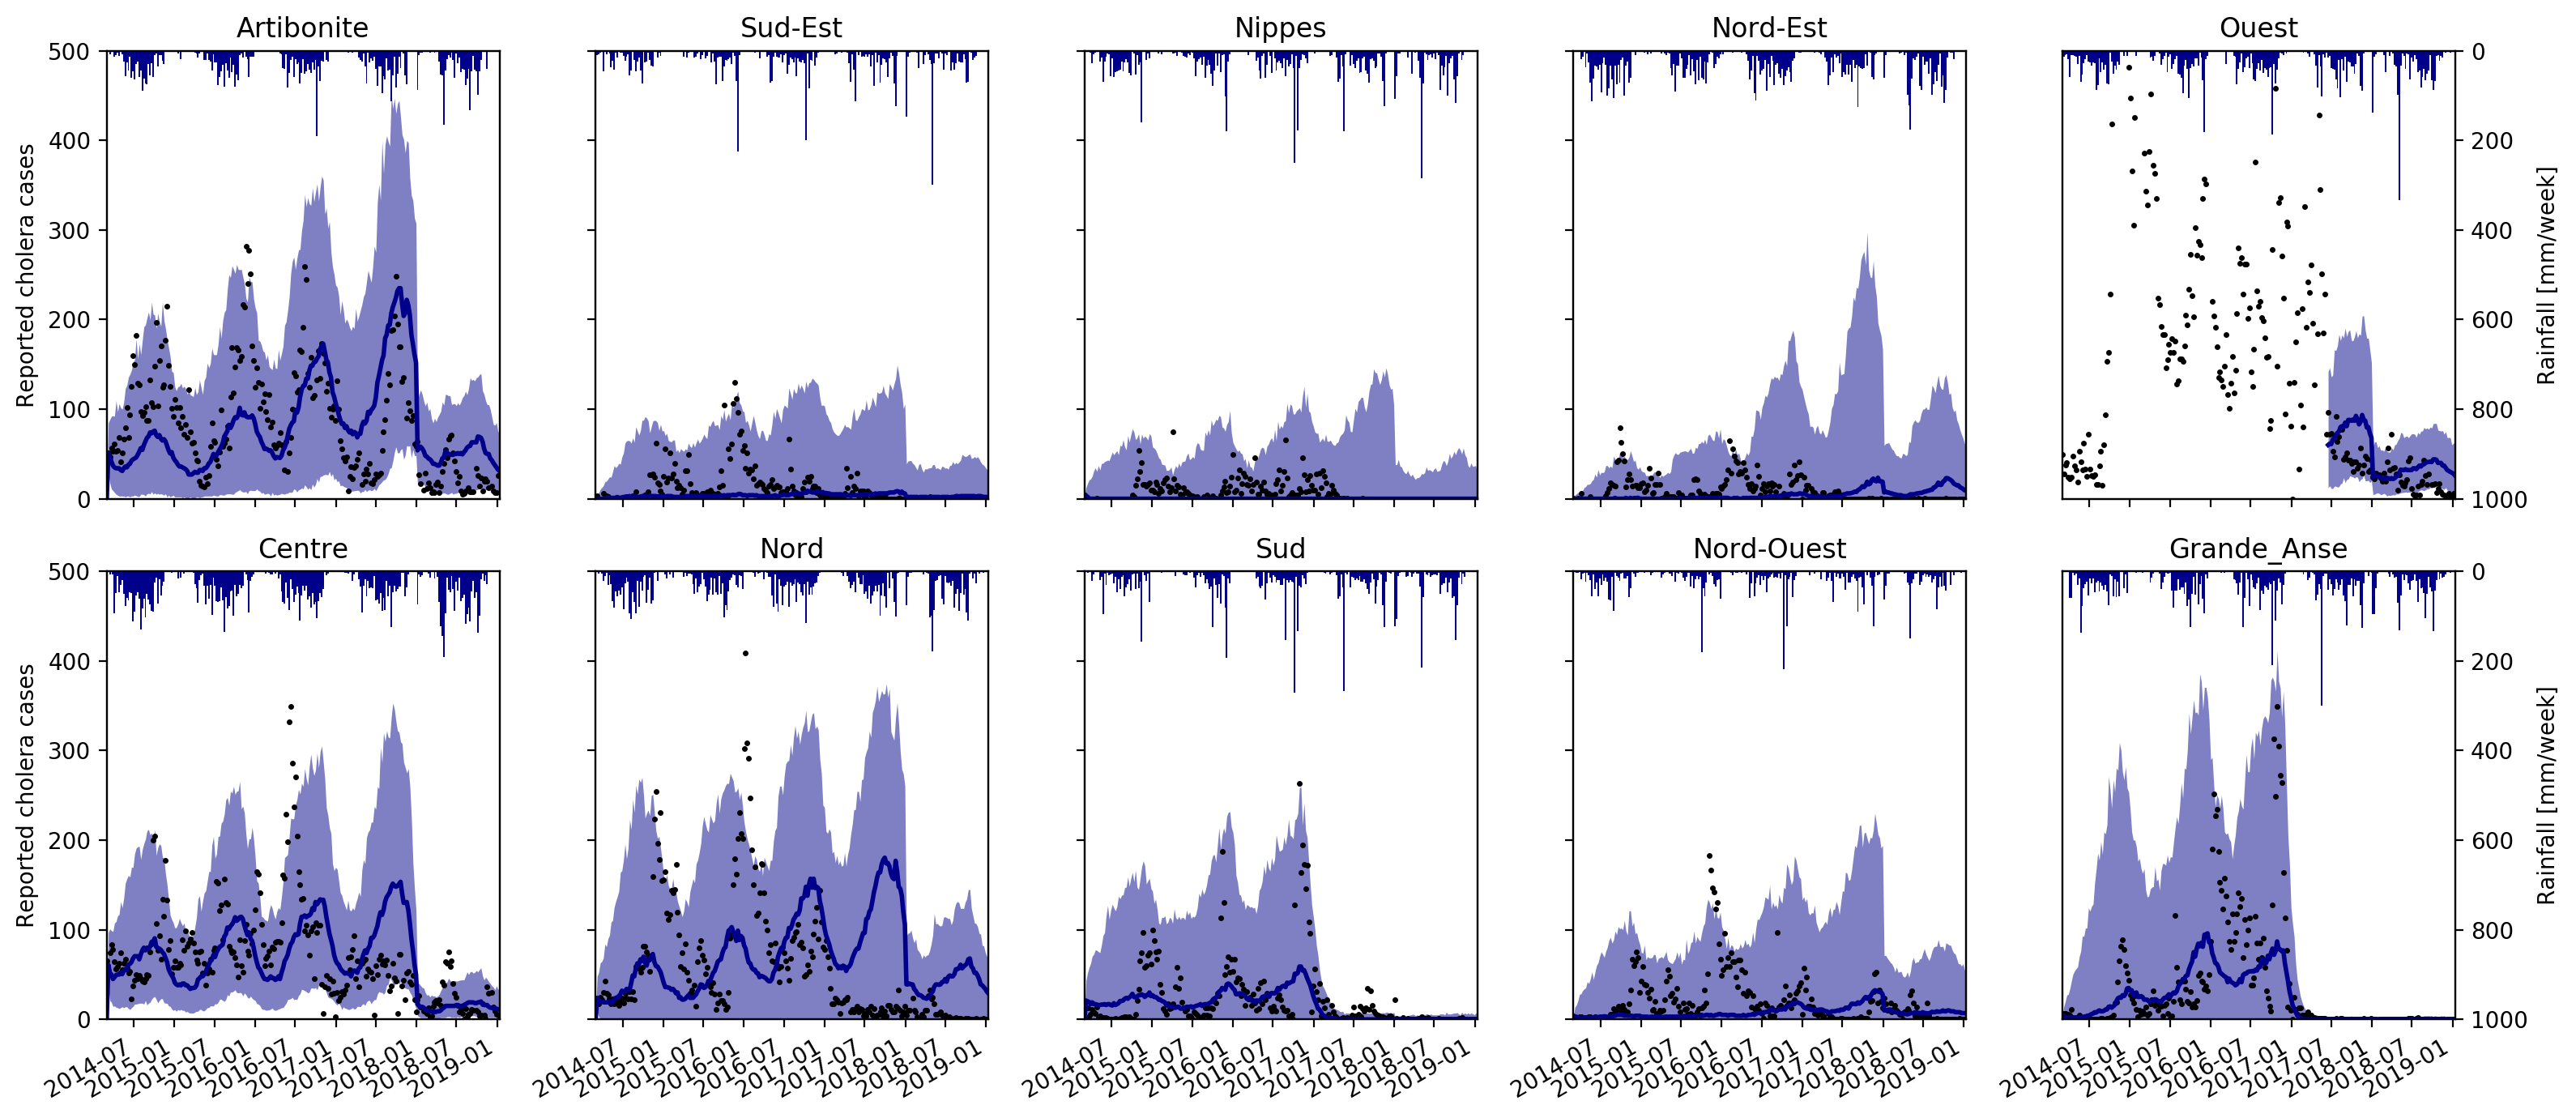
\includegraphics[width=1.0\textwidth]{fig_cholera-haiti-ocv/fit.png}
\caption[Visual assessement of model fit for the selected parameters set]{Visual assessement of model fit for the selected parameters set. The median (blue line) and the q025 and q975 quantiles (shaded area) over 1000 realization of the stochastic model are shown. Weekly reported cholera cases are shown as black dots.}
\label{fitEPFL}
\end{center}
\end{figure*}
After visual convergence is reached in each departements, the departmental best fits is taken as starting points for a country-wide calibration. This mainly affects the mobility parameter $c_i$, which governs the departmental interdependence, as it now calibrated on the actual simulated incidence from other departments. The resulting model fit is shown in fig.~\ref{fitEPFL}. 

\section{Results and discussion}
The common outputs for the exercise are the distribution of time to elimination and probability of elimination in different scenarios. The results are presented below for the six following scenarios, common across modeling teams:
\begin{itemize}
	\item \textsc{No vaccination} status quo.
	\item \textsc{National over 2 years} a nation-wide OCV campaign to reach a coverage 70\% double dose coverage, 10\% single dose and 20\% without any vaccine after 2 years.
	\item 	 \textsc{National over 5 years} a nation-wide OCV campaign with the same coverage, but with a slower deployement over 5 years.
	\item \textsc{2 Departments over 2 years} Campaign focusing only on Centre and Artibonite, the two departments with the highest recent incidence of cholera. Vaccines are deployed to reach the same coverage over 2 years.
	\item \textsc{3 Departments over 2 years} Same as above, but with the addition of Ouest department.
	\item \textsc{National over 2 years, high coverage} same as the National over 2 years, but with a much higher coverage of 95\% two doses, 1.67\% one doses and 3.33\% no vaccination.
\end{itemize}
These scenarios are summarized in in fig.~\ref{fig:deploy} in terms of cumulative number of doses deployed.

\begin{figure}
\begin{center}
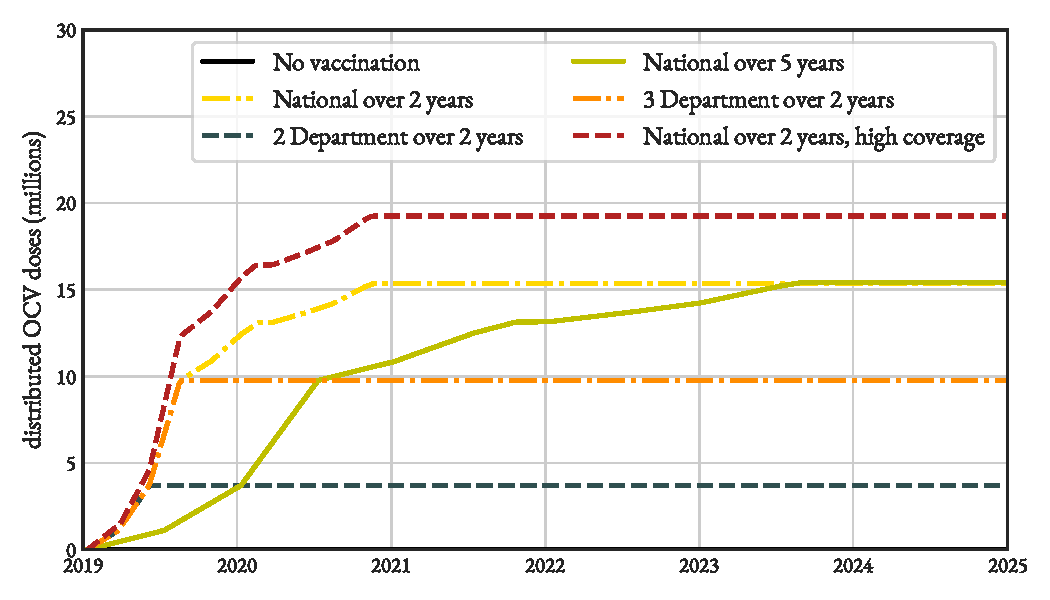
\includegraphics{fig_cholera-haiti-ocv/haiti-deploy.pdf}
\caption[Rate of vaccine doses deployment in each considered scenarios][5\baselineskip]{Rate of vaccine doses deployment in each considered scenarios.}\label{fig:deploy}
\end{center}
\end{figure}

The results in terms of probability of elimination and incidence are shown in fig.~\ref{fig:OCVresults}\marginnote{Only results from our model are presented here. Due to the difficulty of the exercise, the results across teams were quite different, and the reader is referred to \textcite{Lee:AchievingCoordinatedNational:2020} and its supplement to compare the results with the other modeling teams.}. Only a limited long-term impact of the \textsc{2 departments} scenarios is projected. However, all \textsc{national} scenarios considered were projected to lead to elimination, despite the limited vaccine efficacy and coverage. The \textsc{2 departments} and \textsc{3 departments} scenarios exhibit a probability of elimination of about 9.6\% and 48\% respectively (compared to 4.1\% in the status quo scenario). The important impact of adding Ouest to the campaign is due to the department's population, around 4\textsc{m}, which represents about 40\% of the Haitian population. While a slower timing decreases slightly the probability of elimination, it is noted that coverage is far more important than speed for these vaccination campaigns.

\begin{figure*}[h!]%[htbp]
\begin{center}
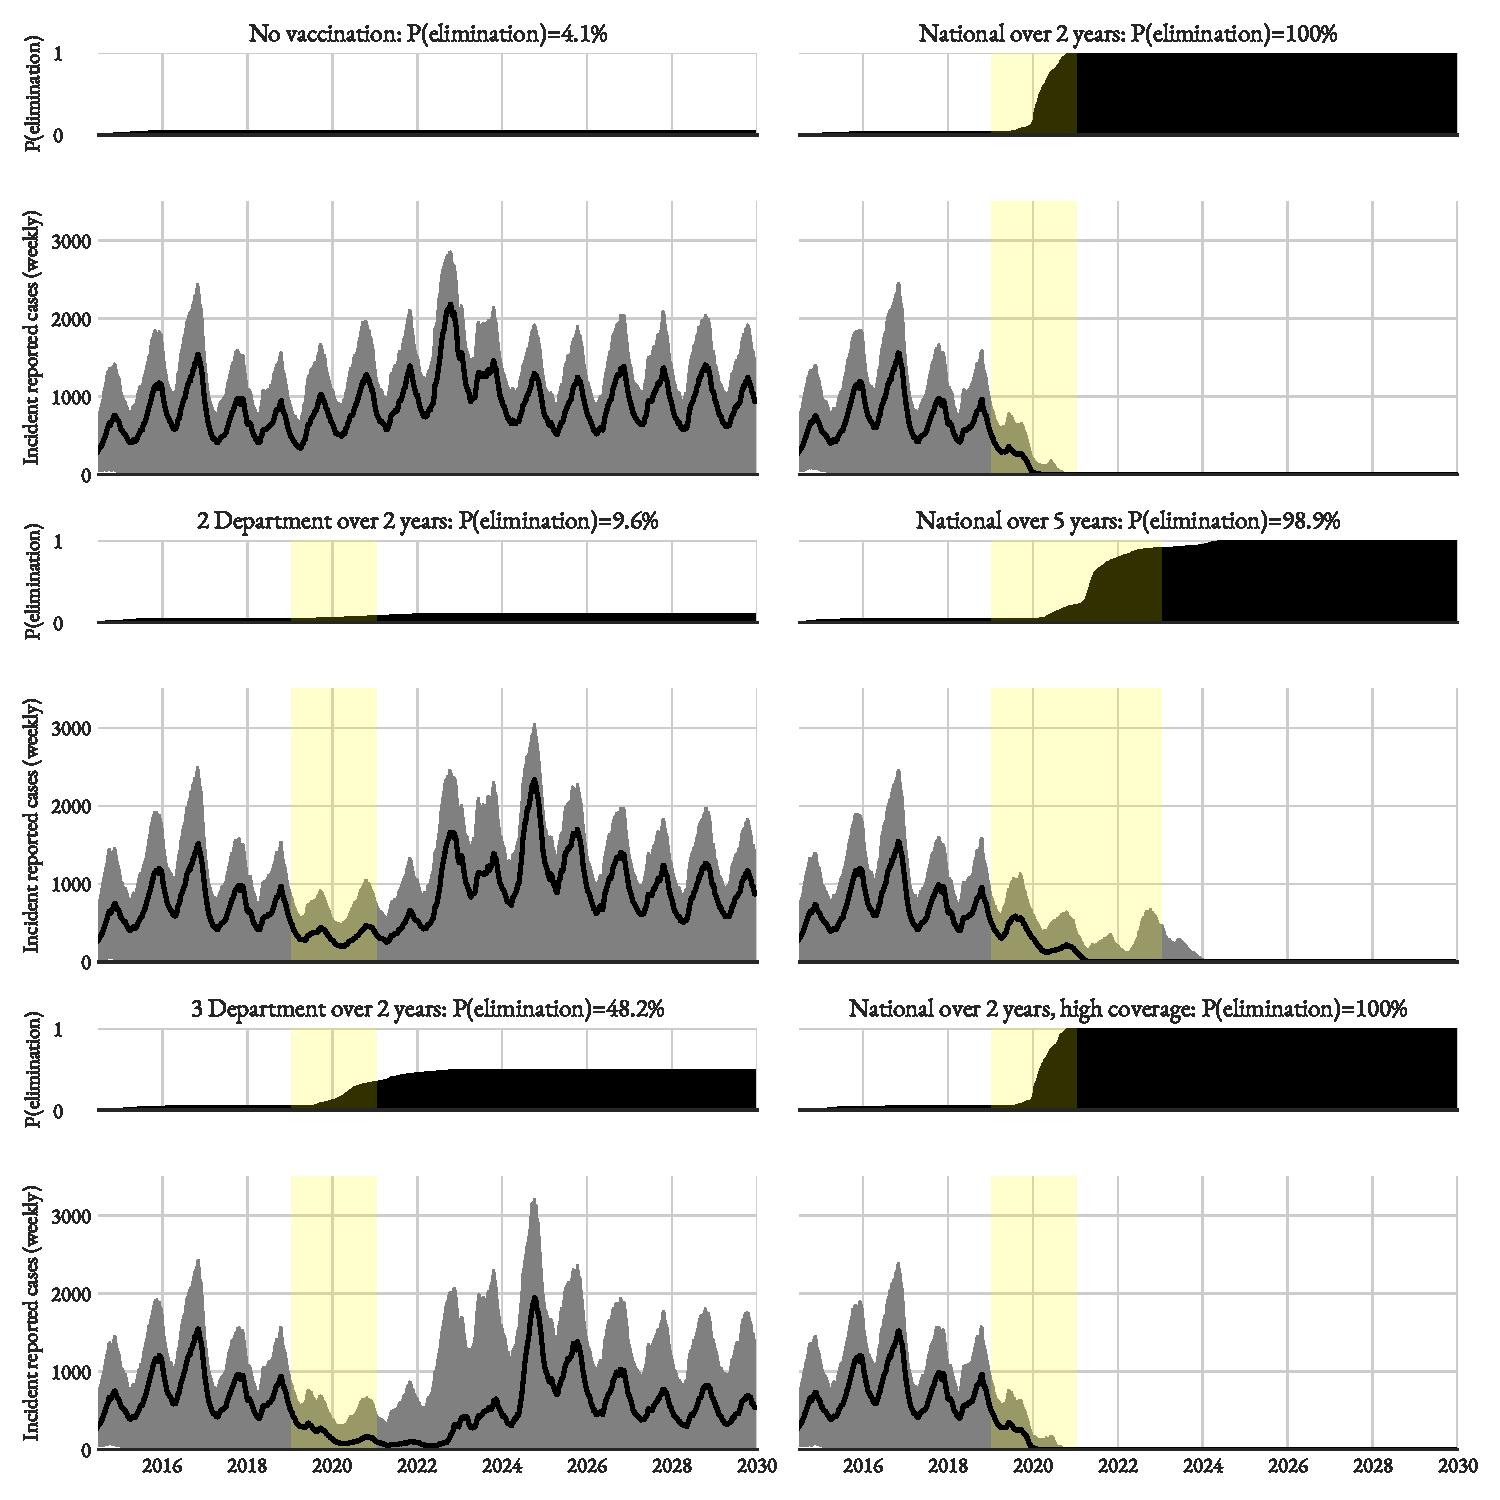
\includegraphics{fig_cholera-haiti-ocv/haiti-scn.pdf}
\caption[Model results: probability of cholera elimination after mass vaccination campaigns]{Modeling results for the considered mass vaccination campaign scenarios, with the weekly reported cases (median and 95\% confidence interval), and cumulative probability of elimination over time. The timing of the vaccine distribution in each scenario is highlighted in yellow.}
\label{fig:OCVresults}
\end{center}
\end{figure*}
 
Haiti has seen no laboratory-confirmed cases of cholera from February 2019. This has sparked claims of cholera elimination, which would mean that the Americas would be free from Cholera. However in the model results, the probability of elimination in the no vaccination scenario is very low (4.1\%). It is always very difficult to predict or explain disease transmissions, and it is even harder for elimination. Possible explanations for the discrepancy observed between what is projected by the model and what happened are (i) issues in the model design, especially concerning the mobility acting as a constant additive pressure for the introduction of cholera cases, hence lowering the probability of extinction; this was done purposefully to sustain transmission as it improved model fit and it was not believed Haiti to be close to elimination at that time, (ii) transmission parameters values error might have biased the estimate of the susceptible population on March 1, 2014, as the absence of serosurvey makes the correct estimation of this quantity critical, (iii) not giving enough weight to the decrease in reported cases from 2017\footnote[][-1.5\baselineskip]{a 90\% decrease of reporting is necessary for the model to replicate the decline in cases. However, it is highly unlikely that the observed decrease in cases is solely due to changes in the reporting process.}, (iv) WaSH interventions and rapid response teams that have been put in place in Haiti and of which have intensified in the last few years\cite{Rebaudet:CaseareaTargetedRapid:2019} might have played a role in disease elimination.
  
 Further work must be performed to study the reasons behind the surprising (to us and other modeling groups, one year before) elimination of cholera from Haiti, and to assess all factors, including WaSH interventions, environmental drivers and socio-economic changes in an unified modeling framework. Effort to investigate this (using the same methods presented for \textsc{covid}-19 in \textsc{Chapter~5}) have been started, but the project has been disrupted owing to \textsc{covid}-19 pandemic, which is the focus of the three remaining chapters.
 


%\part{Scientific and Public-Health response to the COVID-19 pandemic}
%\begin{fullwidth}
\chapter[Assessing the impact of non-pharmaceutical interventions on SARS-CoV-2 transmission in Switzerland]{Assessing the impact of non-pharmaceutical\\ interventions on SARS-CoV-2 transmission\\ in Switzerland}
\chaptermark{Assessing the impact of non-pharmaceutical interventions on covid-19 transmission}
\label{ch:covid-switzerland-npi}

Following the rapid dissemination of \textsc{covid}-19 in Switzerland, large-scale non-pharmaceutical interventions (NPIs) were implemented by the cantons and the federal government between February 28 and March 20, 2020. Estimates of the impact of these interventions on SARS-CoV-2 transmission are critical for decision making in the present and future outbreaks. The aim of this chapter is to assess the impact of these NPIs on disease transmission by estimating changes in the basic reproduction number $R_0$ at national and cantonal levels in relation to the timing of these NPIs. For the whole country and eleven cantons, the time-varying $R_0$ is estimated by fitting a stochastic transmission model explicitly simulating within-hospital dynamics. The dataset includes individual-level data from more than 1000 hospitalised patients in Switzerland and public daily reports of hospitalisations and deaths. The national $R_0$ is estimated to be 2.8 (95\% confidence interval 2.1–3.8) at the beginning of the epidemic. Starting from around March 7, a strong reduction of the time-varying $R_0$ is found, with a 86\% median decrease (95\% quantile range [QR] 79–90\%) to a value of 0.40 (95\% QR 0.3–0.58) in the period of March 29 to April 5. At the cantonal level, $R_0$ decreased by between 53\% and 92\% over the course of the epidemic. Reductions in time-varying $R_0$ were synchronous with changes in mobility patterns as estimated through smartphone activity, which started before the official implementation of NPIs. Most of the reduction of transmission is inferred to be attributable to behavioural changes as opposed to natural immunity, the latter accounting for only about 4\% of the total reduction in effective transmission. As Switzerland considers relaxing some of the restrictions of social mixing, current estimates of time-varying $R_0$ well below one are promising. However, as of April 24, 2020, at least 96\% (95\% QR 95.7–96.4\%) of the Swiss population remains susceptible to SARS-CoV-2. These results warrant a cautious relaxation of social distance practices and close monitoring of changes in both the basic and effective reproduction numbers.

This chapter is based on:
\longfullcite{Lemaitre:AssessingImpactNonpharmaceutical:2020}, and J. Perez-Saez shares co-authorship of the work. It  is referred in the following as the postprint (and its supplementary information \textsc{si})
\end{fullwidth}

\section{Introduction}
As of May 13, 2020, the ongoing coronavirus disease 2019 (\textsc{covid}-19) pandemic caused by severe acute respiratory syndrome coronavirus 2 (SARS-CoV-2) has resulted in more than 4.1 million cases and 280,000 deaths globally\cite{WHO:WHOSituationReport:2020}. Independent estimates of the basic reproduction number $R_0$ for SARS-CoV-2 from the initial phases of the epidemic in China, Europe and the United States have generally ranged from 2–3\cite{Riou:PatternEarlyHumantohuman:2020} with doubling times on the order of 2–4 days. In response to the rapid increase in reported cases and hospitalisations, most countries have implemented non-pharmaceutical interventions (NPIs), including compulsory face mask use, border and school closures, quarantine of suspected and confirmed cases, up to population-wide home isolation\cite{HITCOVIDTeam:HealthInterventionsTracking:2020}. An observation study conducted in Hong Kong during this pandemic estimated that social distancing measures and school closures reduced \textsc{covid}-19 transmission, as characterised by the effective reproductive number, by 44\%\cite{Cowling:ImpactAssessmentNonpharmaceutical:2020}. Comparable reductions have been observed in many different settings\cite{Flaxman:Report13Estimating:2020}. Making decisions around relaxing NPIs requires both a careful assessment of the level of pre-relaxation transmission (e.g., $R_0$) and quantification of the expected increase in transmission from relaxation of different NPIs. 

From the initial reported case on February 24 to April 29, Switzerland reported more than 24'400 laboratory confirmed COVID-19 cases and 1'408 official deaths affecting all 26 cantons\cite{OFSP:RapportSituationEpidemiologique:2020}. The federal government issued a series of special decrees from February 28 banning gatherings of more than 1'000 people culminating on March 20 recommended home isolation (fig.~\ref{fig:covid-ch-data}). One month after the first NPI, daily confirmed case incidence had decreased from a peak of more than 1000 to a daily average of under 170 in the week of April 20–26 (fig.~\ref{fig:covid-ch-data}). Initial reports have suggested a basic reproduction number ($R_0$) of 3.5 at the start of the epidemic, with a decrease of 85\% by March 20\cite[-3\baselineskip]{Flaxman:Report13Estimating:2020}.
\begin{figure*}\centering
  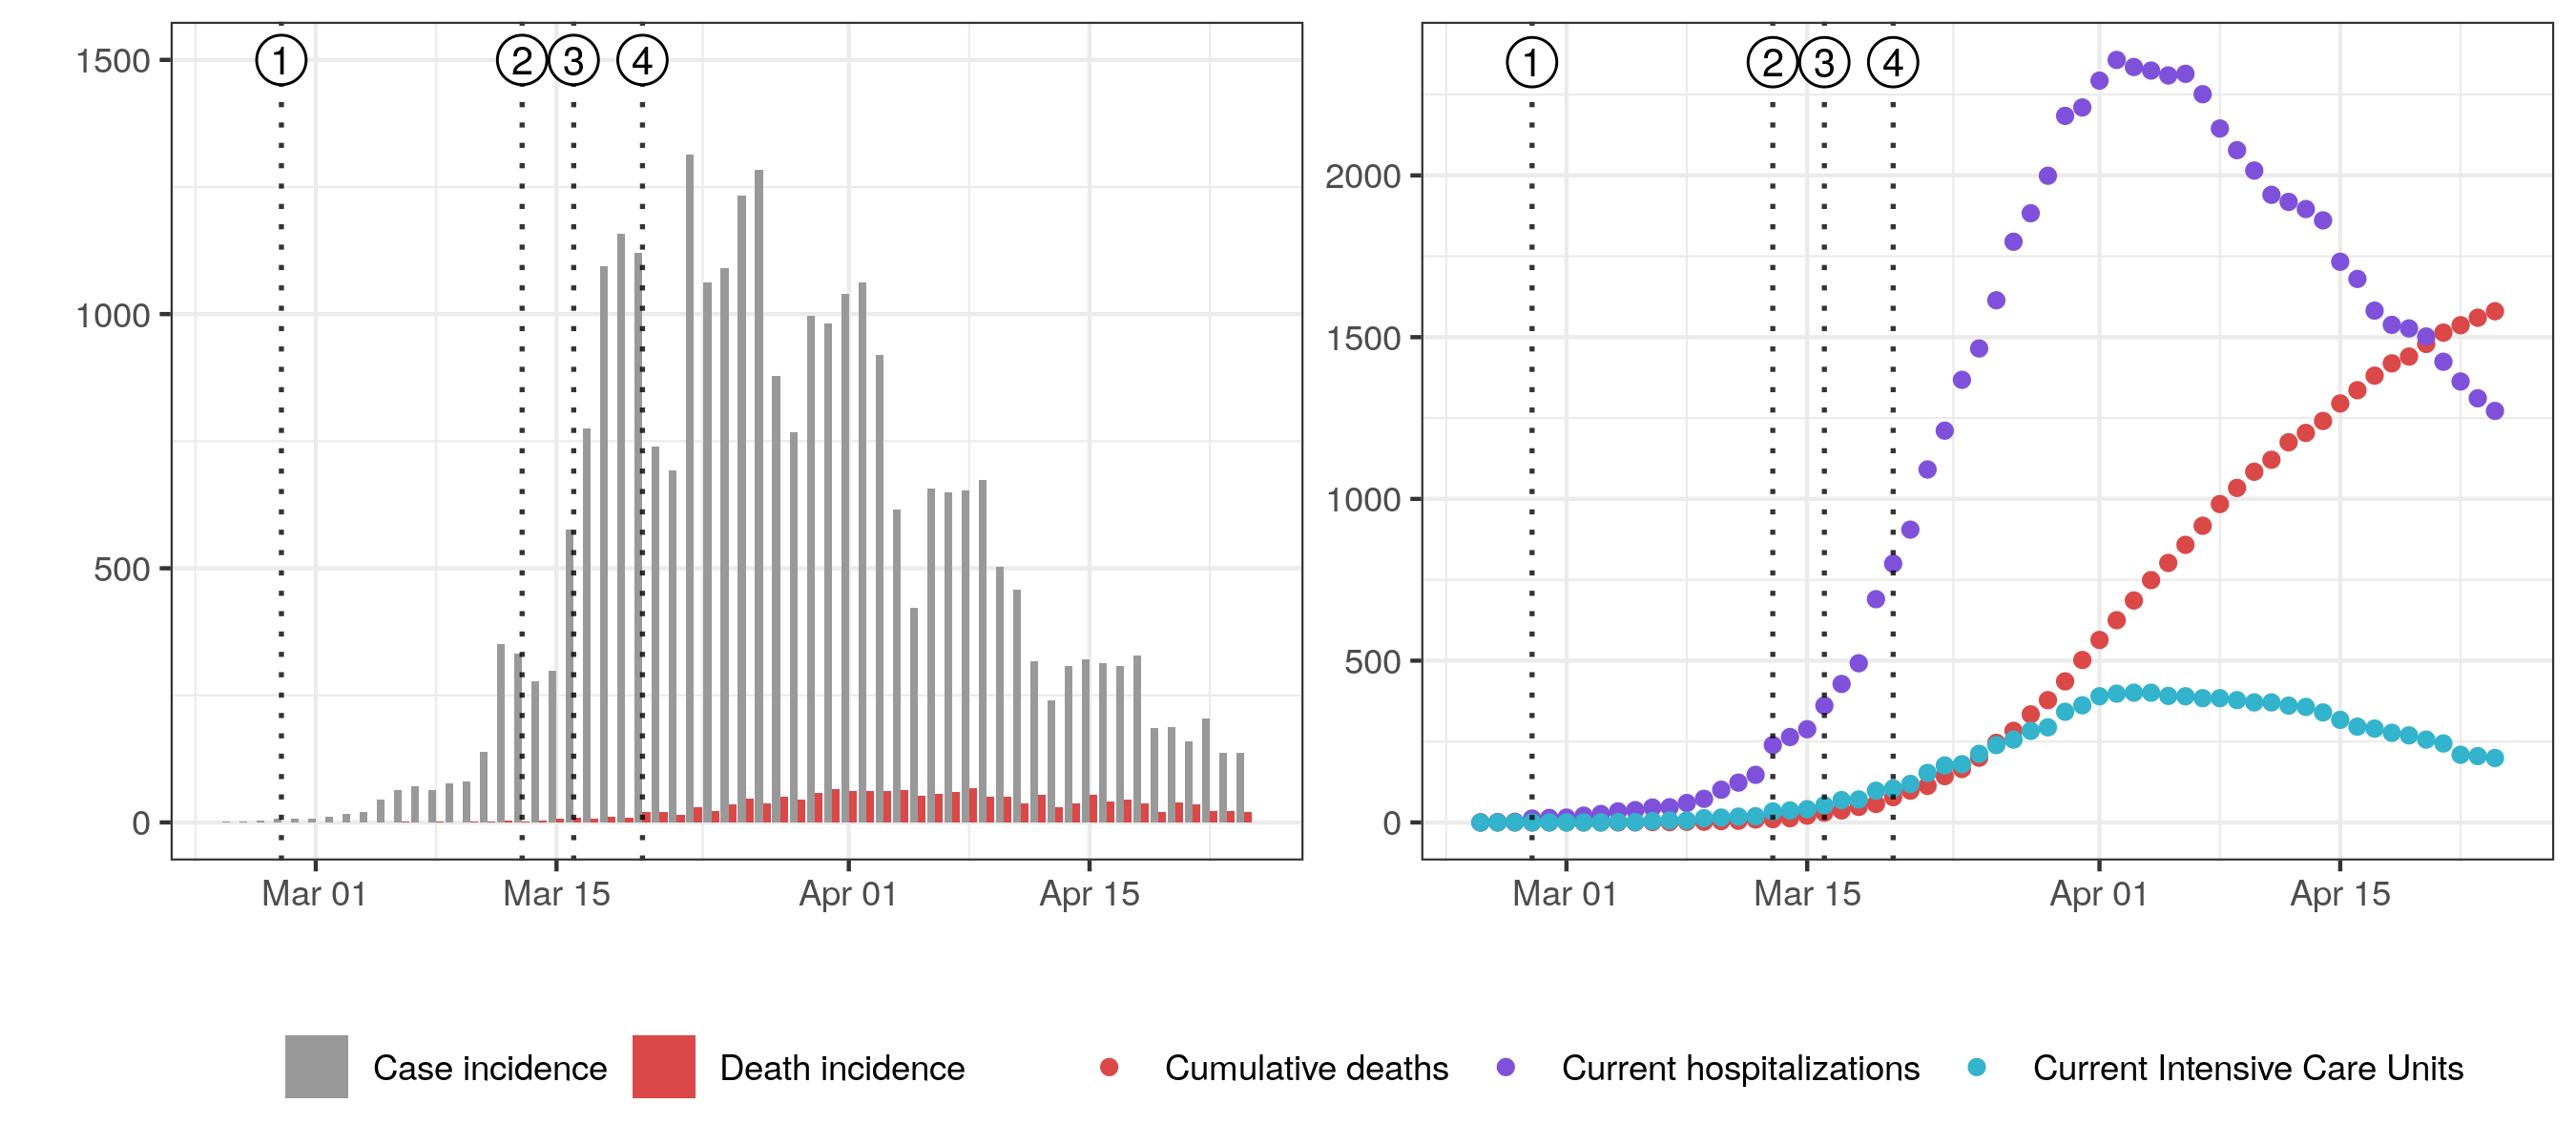
\includegraphics[width=\textwidth]{fig_covid-switzerland-npi/FIGURE_1.png}
  \caption[\textsc{covid}-19 epidemic curve in Switzerland and timing of interventions]{\textsc{covid}-19 epidemic curve in Switzerland and timing of non-pharmaceutical interventions. Dotted lines indicate the issuing of NPIs: (1) ban on gatherings of more than 1'000 people, (2) school closure, (3) closure of non-essential activities, and (4) ban on gatherings of more than five people. Left: Daily case incidence at time of reporting along with death incidence. Right: Current hospitalisations, intensive care units (ICUs) and cumulative deaths. Data from \textcite{Probst:DaenuprobstCovid19casesswitzerland:2020}, and may therefore present inconsistencies with official reports from the Federal Office of Public Health% due to reporting delays.
  }
  \label{fig:covid-ch-data}
\end{figure*}
 However, these estimates, part of a multicountry analysis of NPIs, relied on death incidence and did not account for specifics of the hospitalisation processes in Switzerland. Moreover, changes in $R_0$ were assumed to be on the date of NPI implementation, thus not allowing for the exploration of the relative timing between NPIs and changes in transmission. Furthermore, such delays likely bias the estimate $R_0$. 

NPIs affecting daily activities such as school closures and gathering bans aim at having a direct impact on mobility patterns to reduce potentially infectious social contacts. In other terms, the causal pathway from NPIs to transmission reduction is mediated by changes in mobility. Recent releases of mobility data from smartphone software providers give the possibility to study the associations between the implementation of movement-limiting measures, behavioural change and the related changes in $R_0$. Context-specific data on the degree and speed of compliance with these types of NPIs and associations with the observed decreases in $R_0$ could inform scenario-building should the future reinstatement of measures become necessary. Given that $R_0$ directly represents transmission potential, its quantification enables us to estimate the proportion of reduction in transmission attribuable to behavioral changes. In this sense, tracking of $R_0$ is more suited to study the impact of NPIs than the effective reproduction number $R_{eff}$, which is an aggregate measure of transmission capturing aspects of both infectious contacts and of population susceptibility. 

Here, the goal is to estimate the changes in $R_0$ over the course of the epidemic at both the national and cantonal levels using detailed data on hospitalisations and deaths from Switzerland between February 24 and April 24. In order to understand the estimated changes in $R_0$, its relationship with the timing of NPIs and human mobility estimates derived from cell phone data is explored.

\section{Methods}
The setting for the present chapter arose while providing scenario modeling reports, as presented in \textsc{Chapter~4}. CHUV, the hospital coordinating Canton de Vaud response, provided access to individual hospitalization data. The dataset and processing to account for right-censoring are presented in the \textsc{Appendix to Chapter~5}. This dataset allowed for refined estimates of stays in hospital and death processes, which in turn were used as assumptions in a \textsc{covid}-19 model; giving said model sufficient stiffness to estimate $R_0$ in time. Model equations and fixed and inferred parameter values are left in the postprint \textsc{si}.

\subsection{Model and assumptions}
\paragraph{Model Structure} A stochastic compartmental model of the \textsc{covid}-19 epidemic and hospitalisation processes is developed for each canton of Switzerland. The model is structured around the classical S, E, I and R compartments\cite{Kermack:ContributionMathematicalTheory:1927}, and the model diagram is shown in fig.~\ref{fig:covid-ch-diagram}. %Namely, the population is divided in compartments depending on their status with regard to \textsc{covid}-19. 
A susceptible individual $S$ might be exposed after contact with infectious $I$ individuals. Upon exposure, a formerly susceptible individual goes through an incubation period $E$ before becoming infectious $I$. The individual then recovers $R$ and does not participate in transmission anymore. 
%In addition to these dynamics, some proportion of infectected invididuals develop severe disease and among those, some are hospitalised and may advance to needing the intensive care unit. 
In addition to these dynamics, infected individuals have some probability of developing severe symptoms. Estimates derived from data from the canton of Vaud, as shown in the  show a high proportion of deaths outside of hospitals ($\approx 50\%$) hence two pathways are modeled depending if the individual seek  or has access to hospital care.  Some severly infected will be treated in a hospitals after a delay from symptom onset $I_h$. In this case, hospitalization lead to discharge (recovery) or death, either through normal hospitalization ($H_{s}$ and $H_d$ respectively) or passing through Intensive Care Units (ICUs, compartments $U_{s}$ and $U_d$ respectively). Otherwise, severly infected may recover or die without passing through hospitalization, going into compartment $I_d$. There is no need to explicitly model a latent stage where individuals are still asymptomatic but infectious\cite[-8\baselineskip]{Ganyani:EstimatingGenerationInterval:2020,He:TemporalDynamicsViral:2020, Liu:ContributionPresymptomaticInfection:2020} as only hospitalisation and death data is used. The model is implemented as a hidden markov model using the pomp R package\cite[-3\baselineskip]{King:StatisticalInferencePartially:2015}. 
 \begin{figure}[!htb]
\begin{center}
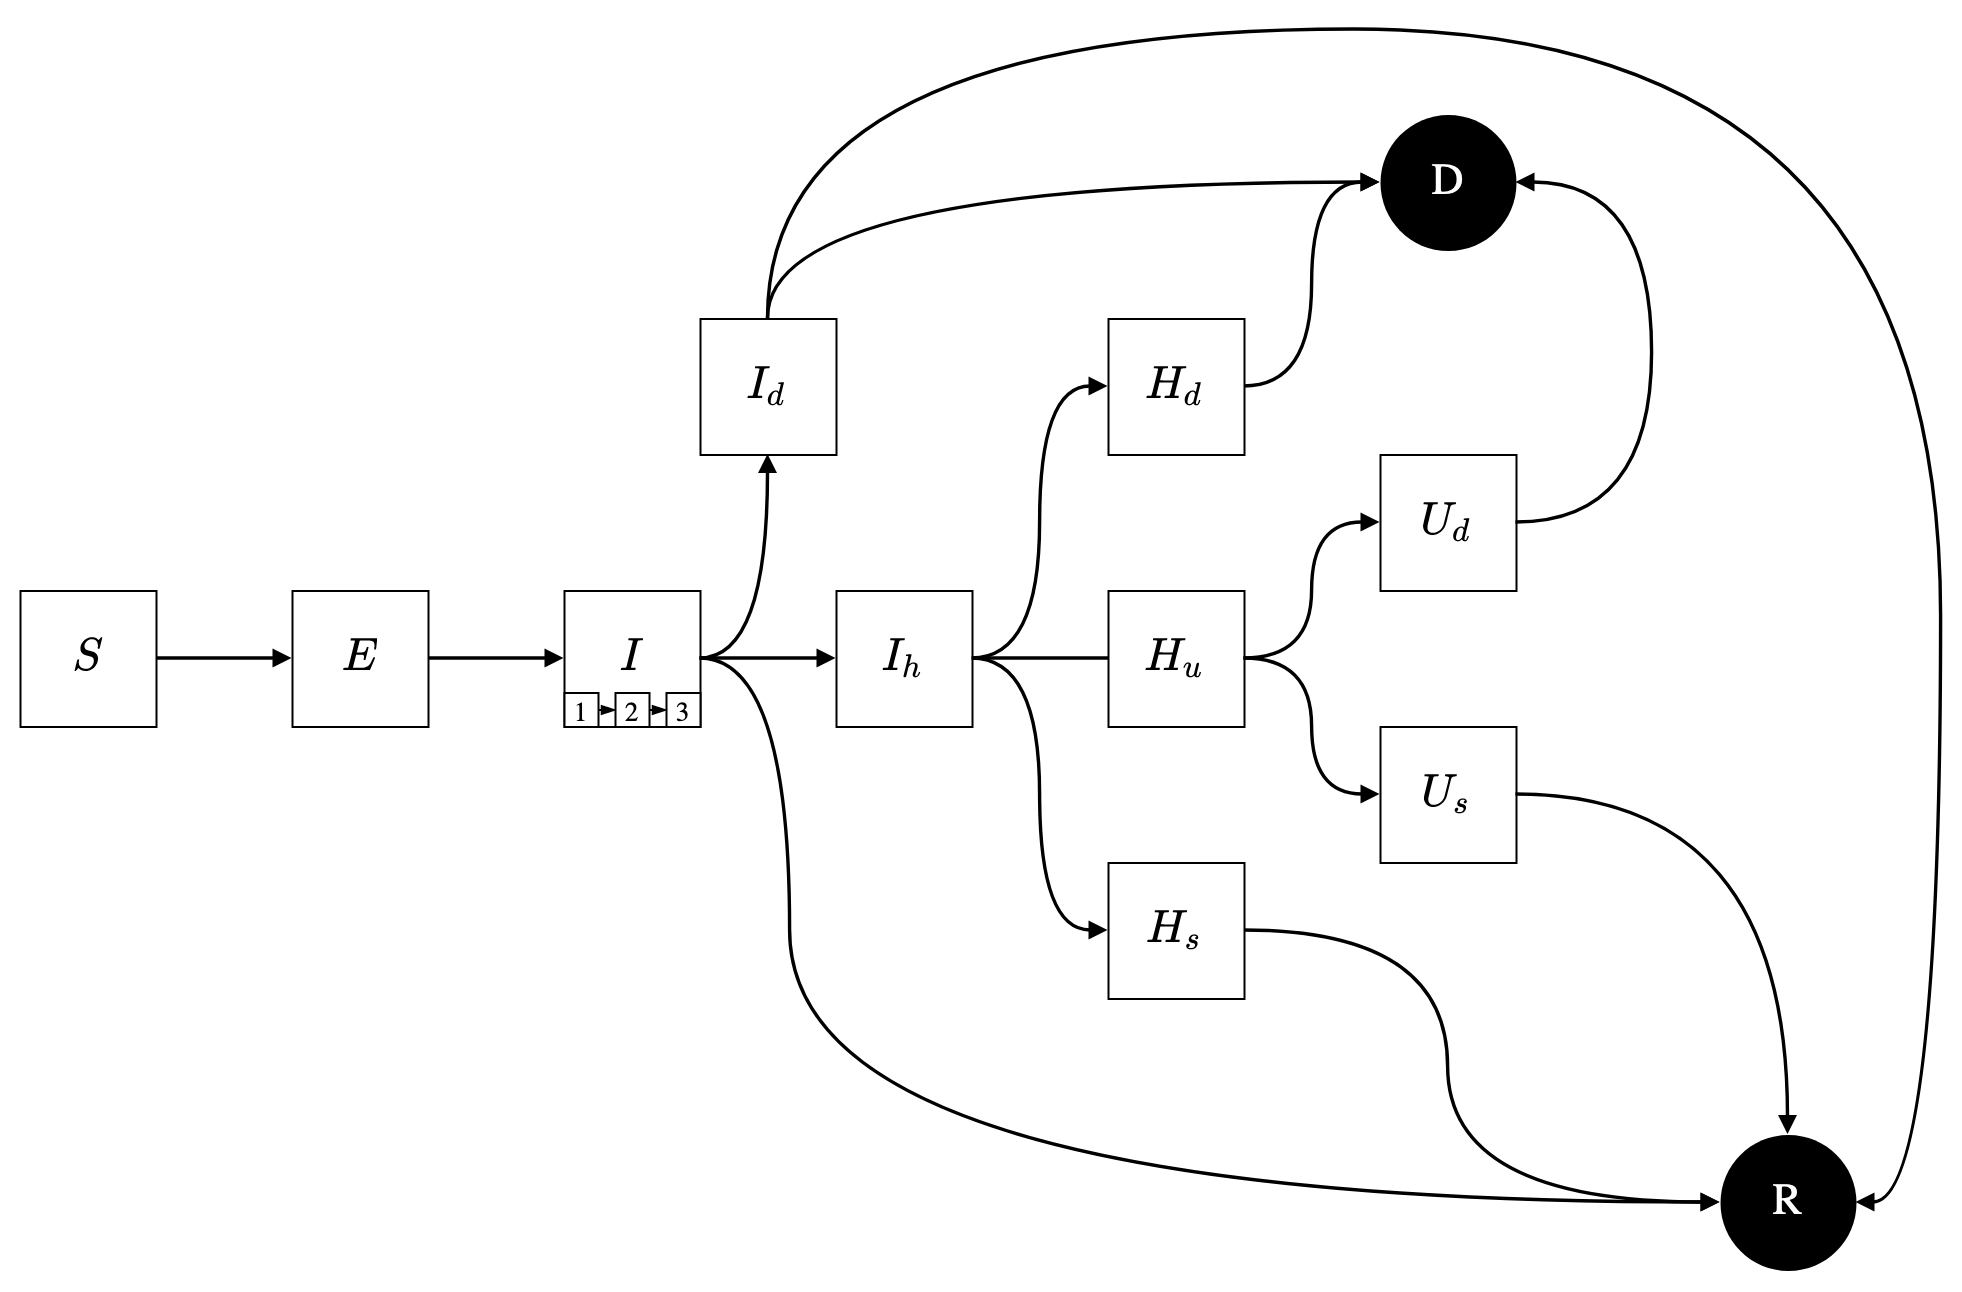
\includegraphics{fig_covid-switzerland-npi/fig_supp/diagram.png}
\caption[Schematic diagram of \textsc{covid}-19 transmission and hospitalization processes]{Schematic diagram of \textsc{covid}-19 transmission and hospitalization processes. There are two sinks: Death $D$ and recovered $R$. Each stage with regard to the disease may be implemented with several compartments (subscript numbered boxes) to better represent the time distribution spent in that stage.}
\label{fig:covid-ch-diagram}
\end{center}
\end{figure}

\paragraph{Assumptions} The reader is referred to the postprint \textsc{si} for the exhaustive description of model transitions and parameters. As parameter indentifiability is needed to capture the dynamics of $R_0$, most of the parameters were fixed to values from the litterature or obtained analyzing the data from Canton de Vaud\footnote[][-3\baselineskip]{As noted by Gostic et al., the accuracy of $R_0$ estimates obtained with the method presented here is sensible to assumptions on model structure and parameters; see \fullcite{Gostic:PracticalConsiderationsMeasuring:2020a}.}.
The transmission model is parameterized assuming a mean generation time of 5.2 days\cite{Ganyani:EstimatingGenerationInterval:2020}, and an exposed and non-infectious duration of 2.9 days\cite{He:TemporalDynamicsViral:2020}, yielding a mean duration of 4.6 days in the infectious compartments.  It is assumed that 7.5\% of infections were severe and would require hospitalisation, that 50\% of deaths happened outside of hospitals (from data on Canton de Vaud described in the \textsc{Appendix}, and data from Geneva collected from OpenZH), that 16\% of those hospitalised would die (data from Vaud, see \textsc{Appendix}), and that the infection fatality ratio (IFR) was 0.75\%, which is in the range of published estimates\cite{Verity:EstimatesSeverityCoronavirus:2020, Russell:EstimatingInfectionCase:2020}. Individual-level data on hospitalised cases from the canton of Vaud is used to estimate the distribution of time spent in the hospital and in the intensive care unit (ICU). Times to discharge and death are estimated using survival models that account for right-censoring of observations (see \textsc{Appendix}). The number of compartments for the linear-chain trick (\ie the shape parameter for the erlang distributed residence time) for each observable hospitalization state was obtained by fitting Erlang distributions to the data of canton de Vaud. To account for right-censoring the model is fitted to the estimated log-normal distributions described in the \textsc{Appendix} instead directly to observed times to events but rather. The rate parameter of the Erlang distributions is calibrated for shape parameters between $1$ and $10$ by minimizing the Kullback-Leibler (KL) divergence between the Erlang and estimated log-normal distributions. The final fit was taken to be the one with the smallest KL-divergence. We found that all hospitalization processes were best represented with exponential distributions (Erlang with shape parameter of $1$)\footnote{In the first preprinted version without the survival analysis, the shape parameters were estimated to be around 2, which highlights the importance of carefully processing data and reasoning about potential biases before using it.}.

\subsection{Data and Inference} 
\paragraph{Dataset} Curated data from OpenZH\cite[3\baselineskip]{openZH:OpenZHCovid19:2020} up to April 24 is used. This dataset included, by canton, the number of hospitalised \textsc{covid} patients, and the cumulative numbers of deaths, cases and hospital discharges; the latter not available for all cantons. The cantonal estimate is focused on cantons that had enough cases and data to obtain meaningful results, keeping 11 of the 26 cantons (Bern, Basel-Landschaft, Basel-Stadt, Fribourg, Geneva, Jura, Neuchâtel, Ticino, Vaud, Valais and Zurich). These cantons account for 66\% of the Swiss population. The national estimate uses curated national aggregate data and thus encompassed all cantons\cite{Probst:DaenuprobstCovid19casesswitzerland:2020}. Unknown parameters the model are fitted using maximum likelihood inference through iterated filtering\cite{Ionides:InferenceDynamicLatent:2015}. No attempt to include confirmed case data into the observation model were made because of the heterogeneous testing strategies adopted across cantons and over time. The model is therefore fitted to death incidence and changes in current hospitalisations using appropriate likelihood functions:
\begin{equation}
\begin{split}
 \text{deaths}(t) &\sim \text{Poisson}(\Delta D(t)) \\
\Delta  \text{hosp}(t) &\sim \text{Skellam}(\Delta H(t), \Delta D_H(t) + \Delta R_H(t)) \\
\end{split}
\end{equation}
\noindent where, $\Delta D(t)$, $\Delta H(t)$, $\Delta D_H(t)$, $\Delta R_H(t)$ are respectively the number of new deaths, hospitalized, and deaths and discharged from hospitals at time $t$, and $\Delta \text{hosp}(t)$ is the difference between the number of current hospitalizations at times $t$ and $t-1$, for which a Skellam distribution\footnote{which represents the difference between two independent random variables, each Poisson-distributed. See \fullcite{Skellam:FrequencyDistributionDifference:1946}.} is choosen. The full log-likelihood of the observation model was taken as the sum of the individual log-likelihoods of the $\Delta \text{hosp}(t)$ and of the $\text{deaths}(t)$. 
The model is calibrated separately for each canton on the daily death and hospitalization until April 24. Hospitalisation incidence data at the cantonal level would have provided more information, but this data was not accessible. Fitting to hospitalisation incidence data, which access was granted in the canton of Vaud, yielded similar results to those when changes in current hospitalisations were used. The majority of model parameters was either derived from Vaud data or from the litterature (see postprint \textsc{si}), it enables the identifiability of the reproduction number $R_0$.
 
 \paragraph{Reproduction number estimation} Time-varying basic reproduction numbers $R_0$ were estimated following a similar approach to Cazelles et al.\cite{Cazelles:AccountingNonstationarityEpidemiology:2018}, recently applied to \textsc{covid}-19 transmission in Hubei\cite{Kucharski:EarlyDynamicsTransmission:2020}. The method aims at inferring the time series of $R_0$\footnote{As mentionned, $R_0$, not $R_{eff}$ is computed as the presented method estimates the basic reproduction number, \ie the expected number of infections generate by one infected individual in a fully susceptible population. To do so, the susceptible and recovered population explicity modeled while other methods usually compute the effective reproduction number in the population by deconvolution on observed data.} that yields model dynamics that are in best agreement with the whole set of available observations. As such, the value of $R_0$ at a given point in time is informed by the whole data, and therefore does not have the limitations of being either “forward looking” or “backwards looking” as it is the case of commonly used statistical methods applied for this purpose\cite{Wallinga:DifferentEpidemicCurves:2004,Cori:NewFrameworkSoftware:2013,Lipsitch:CommentPanLiu:2020}. 
 
The model equations are similar to the previously presented partially-observed Markov Processes models, and are left in the postprint \textsc{si}. The difference lies in the force of infection. Given the state of the system at time \(t\), \(\mathcal{X}_t\), and using the same notations as in \textsc{Chapter~3}, the transition $S \longrightarrow E$ model reads:

\begin{gather}
\begin{aligned}
    \mathbb{P}\left[ \Delta N_{SE}(t) = 1 \mid\mathcal{X}_t\right] &=  \underbrace{\beta(t)  \frac{I_1(t) + I_2(t) + I_3(t)}{P}}_{\text{Force of infection} S(t)} \Delta t + o(\Delta t)\\
    \end{aligned}
\end{gather}

Time-varying $R_0(t) = \beta(t)/(3r_I)$ is modelled as a geometric random walk defined by its calibrated variance, where $\beta$ is the transmission parameter and $1/(3r_I)$ is the mean duration spent in the infectious compartments $I_1$ to $I_3$. Once the time series was inferred, the timing and slope of changes in $R_0$ is evaluated by using linear changepoint models\cite{Lindelov:McpPackageRegression:2020}. The null model corresponded to a linear decrease between two plateaus corresponding to the baseline value at the start of the epidemic and a low value after the implementation of NPIs. To allow for different slopes in the decreasing phase of $R_0$, models with one and two additional breakpoints (corresponding to two and three different slopes) are also fitted, and the best model was selected using Bayesian model selection based on leave-one-out cross-validation (details in section 6 of the postprint \textsc{si}). 

The estimated changes in $R_0$  were constrasted with changes in activity-related mobility data produced by Google\cite{GoogleLLC:GoogleCOVID19Community:2020}. Changes in activity were expressed as relative changes with respect to a baseline computed as the median over a 5-week period from January 3 to February 6. Mobility changes were computed for different categories: grocery and pharmacy, parks, transit stations, retail and recreation, residential, and workplace. Mobility estimates were based on smartphone-based geo-location location data (GPS, WiFi connections, Bluetooth) from users who activated Location History for their Google Account. These data were used to determine changes in the number of visits to and length of stays in locations categorized into the above-mentioned types. The dataset therefore only covers a sample of the Swiss population who use smartphones, the latter representing around 80\% of the total population in 2020\cite{ODea:SmartphoneUsersSwitzerland:2020}. Gaps in the dataset were filled with linear interpolation and a 7-day moving average was applied to smooth out weekly seasonality in activities. The cross-correlation between changes in $R_0$ and the averaged changes in each type of activity was computed with lags up to 10-days. Changes in $R_0$ were computed based on location-specific baselines taken as the mean value of $R_0$ from the beginning of the simulations, 5 days before the first reported case in each canton, until March 8. Changepoint models are employed identify dates of change in mobility patterns and in $R_0$. \marginnote[-5\baselineskip]{All data and code except for individual hospitalisation data from Canton of Vaud have been deposited on Zenodo (\url{doi.org/10.5281/zenodo.3862075}). The change point analysis, model fit and additional results are omitted from this thesis and may be found in the supplementary information of \parencite{Lemaitre:AssessingImpactNonpharmaceutical:2020}}


\section{Results}
\begin{figure*}\centering
  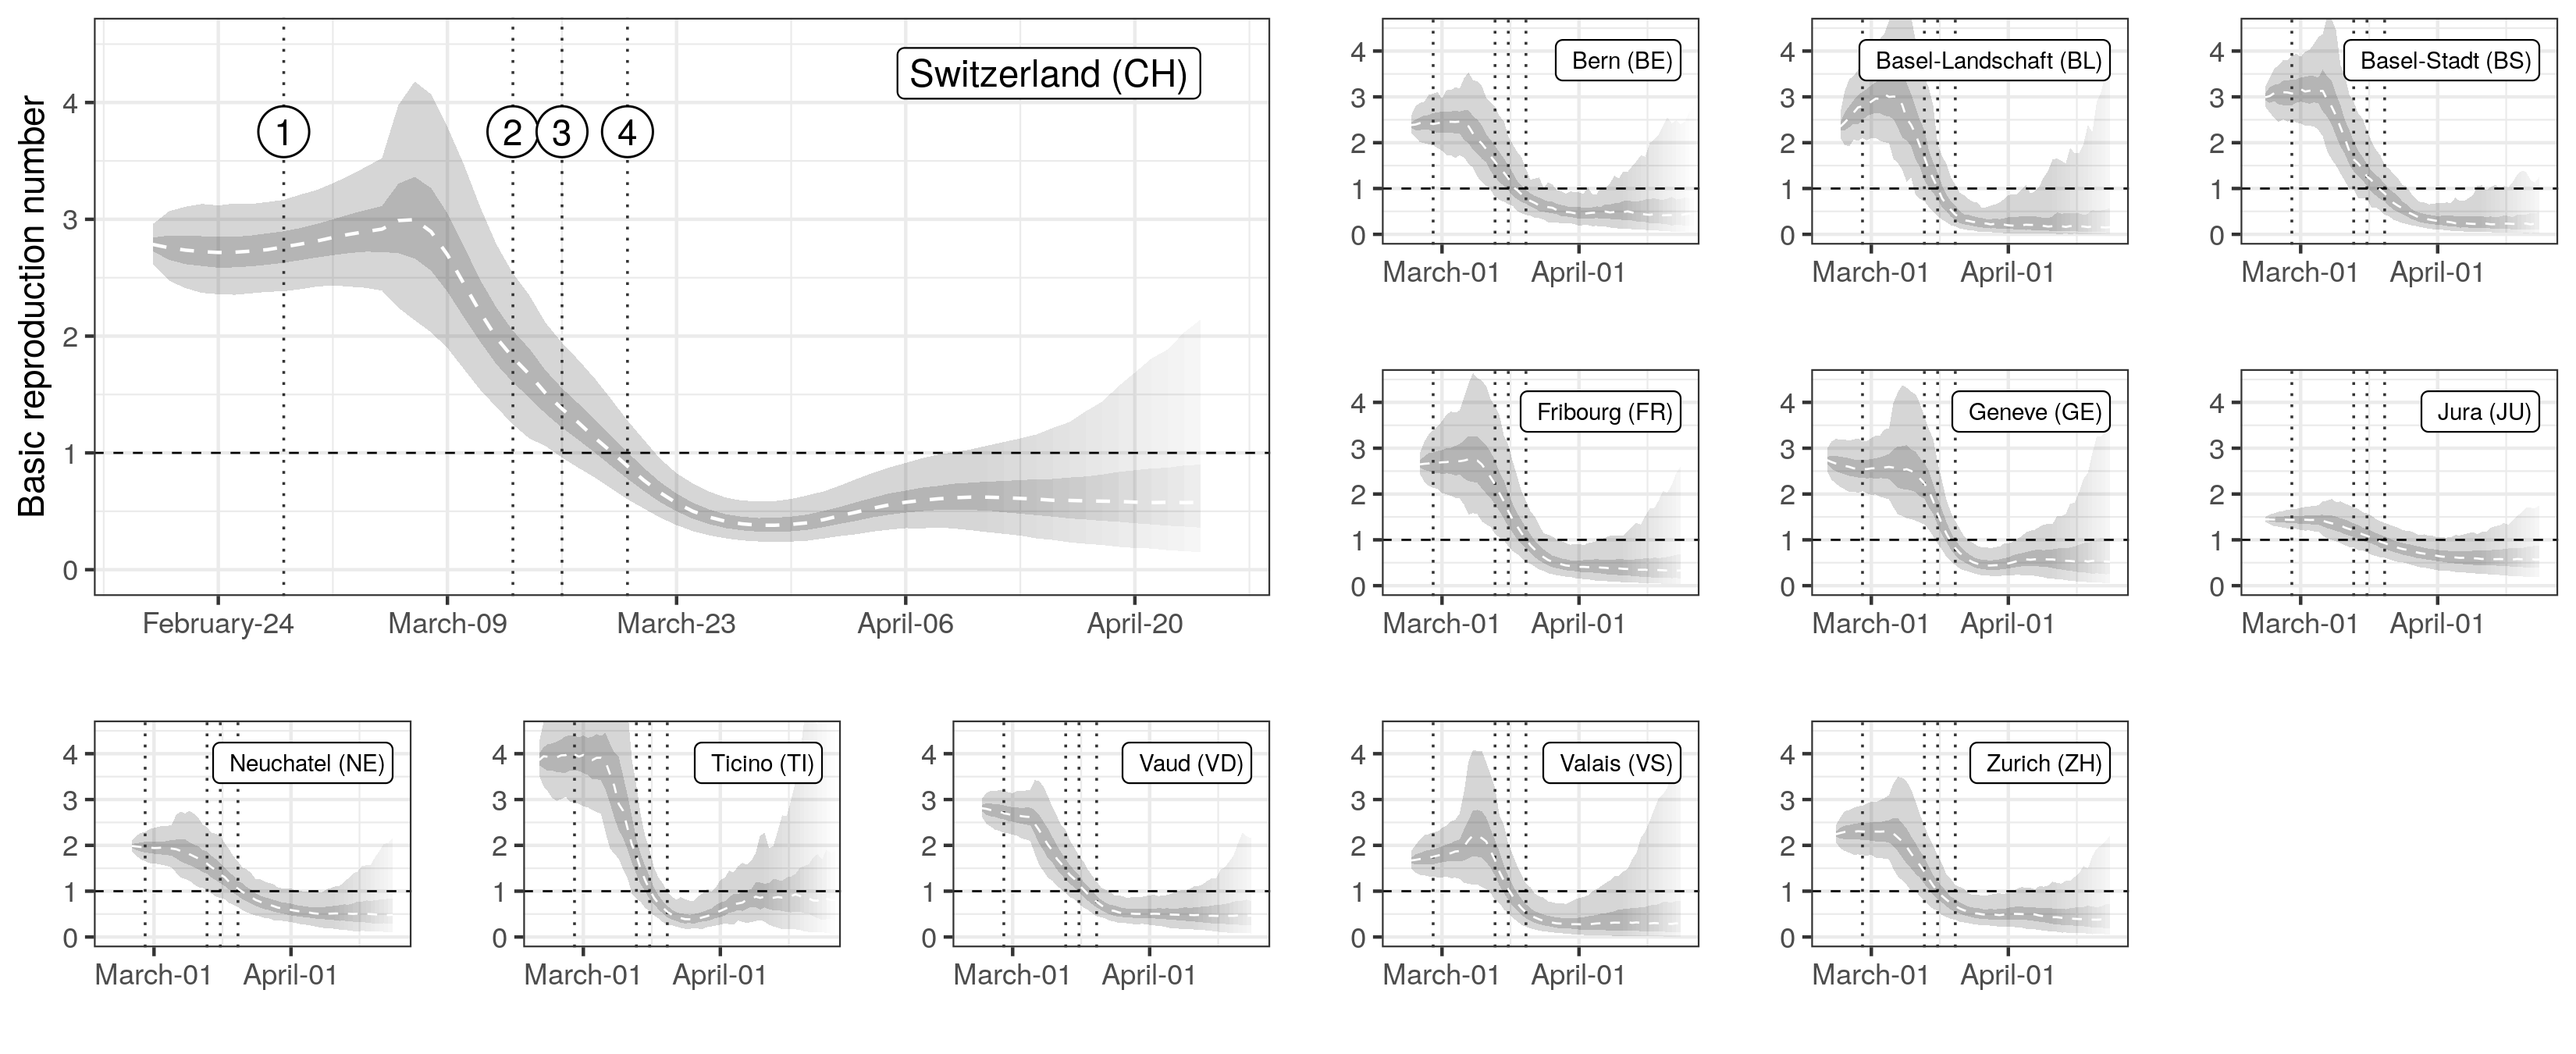
\includegraphics[width=\textwidth]{fig_covid-switzerland-npi/FIGURE_2.png}
  \caption[Estimates of changes in the basic reproduction number $R_0$][-1\baselineskip]{Estimates of changes in the basic reproduction number $R_0$. Median (dashed line), IQR (dark gray) and the 95\% QR (light gray) of the estimated time series of $R_0$ are shown for each canton. Vertical dotted lines indicate the issuing of NPIs as described in fig.~\ref{fig:covid-ch-data}. Transparency at the end of the time series indicates increasing uncertainty (style inspired by the reports of CMMID.}
  \label{fig:covid-ch-r0}
\end{figure*}
Over the study period $R_0$ trends follows a common trajectory nationally and across cantons, starting with a high plateau ($R_0 >2$) in the early stage of the epidemic followed by a rapid reduction starting at the beginning of March, and reaching a low and stable value ($R_0 <1$) from end of March onwards (fig.~\ref{fig:covid-ch-r0}). 

At the beginning of the epidemic, $R_0$ is estimated at 2.8 (95\% confidence interval [CI] 2.06–3.83) at the national level, with cantonal-level values ranging from 2.5 to 3.1 (postprint \textsc{si} tab. 5). The onset of the reduction was estimated to be between March 4 (Basel-Stadt and Vaud) and March 11 (Geneva and Valais) at the cantonal level and on March 7 at the national level (postprint \textsc{si} fig. 11). Overall a strong support is found for the reduction in $R_0$ starting before school closures on March 13 (probability 0.99 at the national level, postprint \textsc{si} fig. 11). Once started, a strong decrease in $R_0$ is estimated at the national (reduction of 0.16/day) and cantonal levels (between 0.14/day in Jura to 0.18/day in Basel-Landschaft) (fig.~\ref{fig:covid-ch-r0}). No strong support was found for changes of slope during the decrease phase at either at the national or cantonal levels except for Bern, Basel-Stadt and Vaud, for which additional changes in slopes were inferred towards the stabilisation of $R_0$ at low values (postprint \textsc{si} tab. 7).\marginnote[0\baselineskip]{Additional results may be found in the supplementary informations of \fullcite{Lemaitre:AssessingImpactNonpharmaceutical:2020}.} $R_0$ in Switzerland has been estimated to drop below 1 on March 19 (95\% CI March 16–22) with individual cantons meeting this threshold between March 16 (Basel-Stadt) and March 20 (Neuchâtel) (postprint \textsc{si} fig. 10). The probability that $R_0$ had already fallen below one was low when schools closed on March 13 (national 0.006, cantonal from $0$ in Geneva to 0.23 in Basel-Landschaft), and high by the time gatherings of five people or more were banned on March 20 (national 0.92, cantonsal from 0.52 in Neuchâtel to 0.99 in Ticino) (postprint \textsc{si} fig. 9). The estimated plateau value of $R_0$ after the reduction, that is, from March 29 to April 10, was of 0.4 (95\% quantile range [QR] 0.3–0.6) at the national level, with median values at the cantonal level ranging from 0.2–0.7 (postprint \textsc{si} tab. 5). At the national level, $R_0$ was reduced by 86\% (95\% QR 79–90\%), with median reductions ranging from 53\% (Jura) to 92\% (Basel-Stadt) at the cantonal level. A gradual reduction in $R_0$ leading to values below one around the third week of March is consistent with the observed reduction of confirmed case incidence in early April, when tarking into consideration the delays due to the incubation period, with median of 5.2 days\cite[-6\baselineskip]{Lauer:IncubationPeriodCoronavirus:2020}, and between symptom onset and reporting\cite[-2\baselineskip]{Bi:EpidemiologyTransmissionCOVID19:2020}. Similarly, the inflection in the number of current hospitalisations and ICU usage in early April also supports $R_0$ dropping below one in mid-March. 

\begin{figure*}\centering
  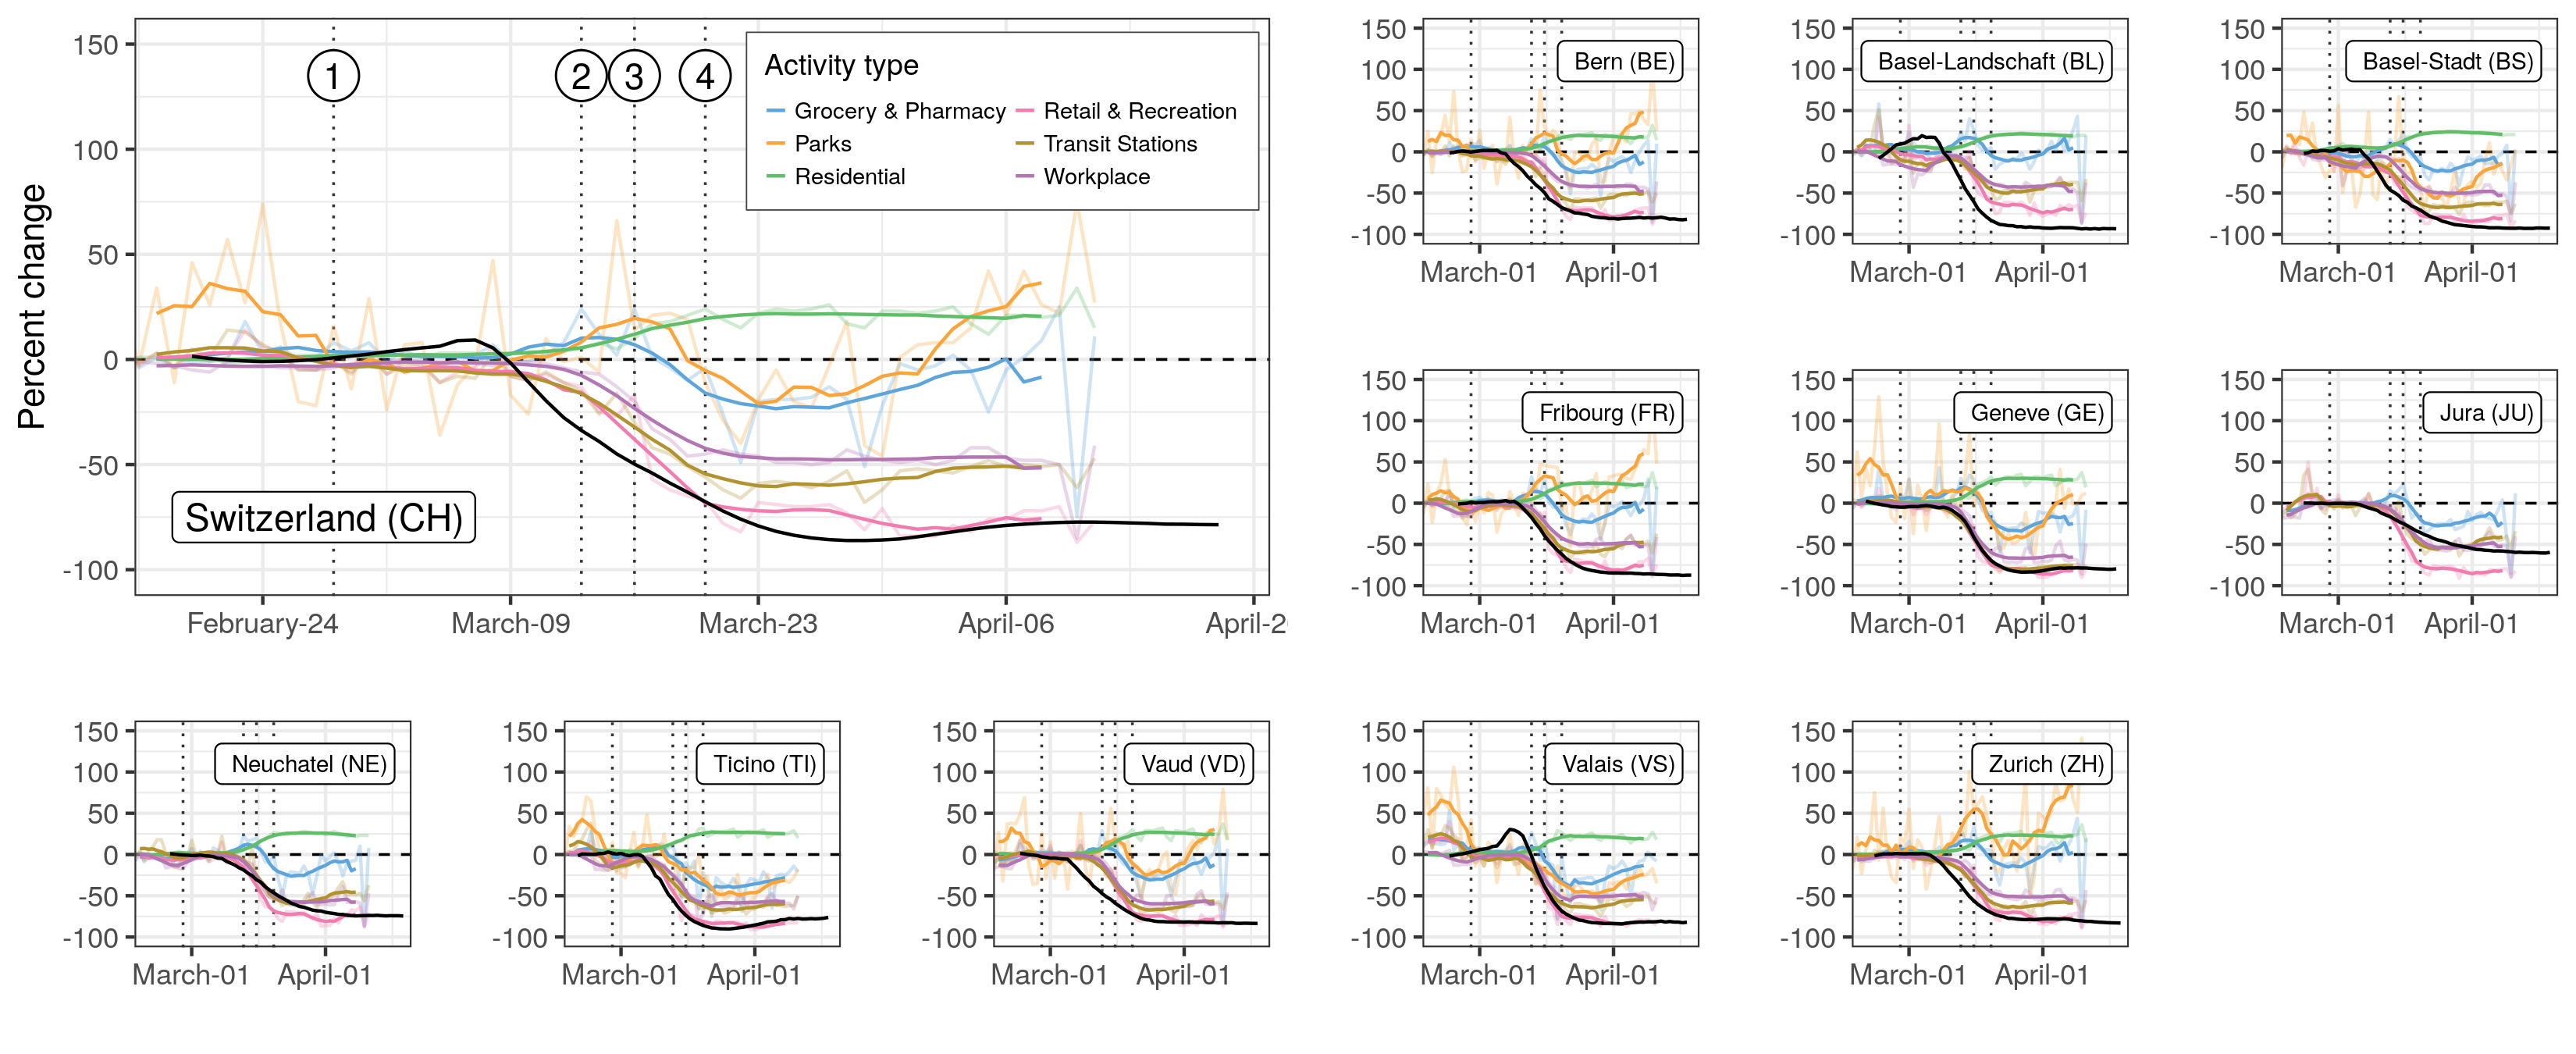
\includegraphics{fig_covid-switzerland-npi/FIGURE_3.png}
  \caption[Changes in mobility patterns and $R_0$][-1\baselineskip]{Changes in mobility patterns and $R_0$.Changes in mobility with respect to baseline are shown by activity type in terms of the daily values (transparent lines) and 7-day rolling mean (full lines), against the median estimate of $R_0$ (black line). Vertical dotted lines indicate the issuing of NPIs as described in fig.~\ref{fig:covid-ch-data}.}
  \label{fig:covid-ch-mobility}
\end{figure*}

Activity-related mobility patterns changed markedly in all cantons since the beginning of the epidemic (fig.~\ref{fig:covid-ch-mobility}). Mobility related to work, retail and recreation, and transit stations dropped by 50\% to 75\% at the national level, with cantonal-level reductions ranging from 30\% to 80\% depending on activities. Residential-related mobility increased across cantons between 20\% and 30\%. Strong support is found for mobility changes starting simultaneously for all activity types within each canton. Changes in mobility are estimated to have started between March 6 to 14 for all cantons (postprint \textsc{si} fig. 12), thus finding strong support for changes starting before school closure on March 13 (national-level mean probability across activities 0.70, cantonal range 0.55–0.99). 

Based on the changepoint models, reductions in $R_0$ likely started (probability 0.76) before observed reductions in mobility at the national level and across cantons (fig.~\ref{fig:covid-ch-mobility}). Changes in $R_0$ were highly correlated with changes in mobility, the strongest associations being with mobility related to work, transit stations, retail and recreation, and residential (cross-correlations >0.9 in all cantons and nationally, fig.~\ref{fig:covid-ch-timing}). 
\begin{figure*}\centering
  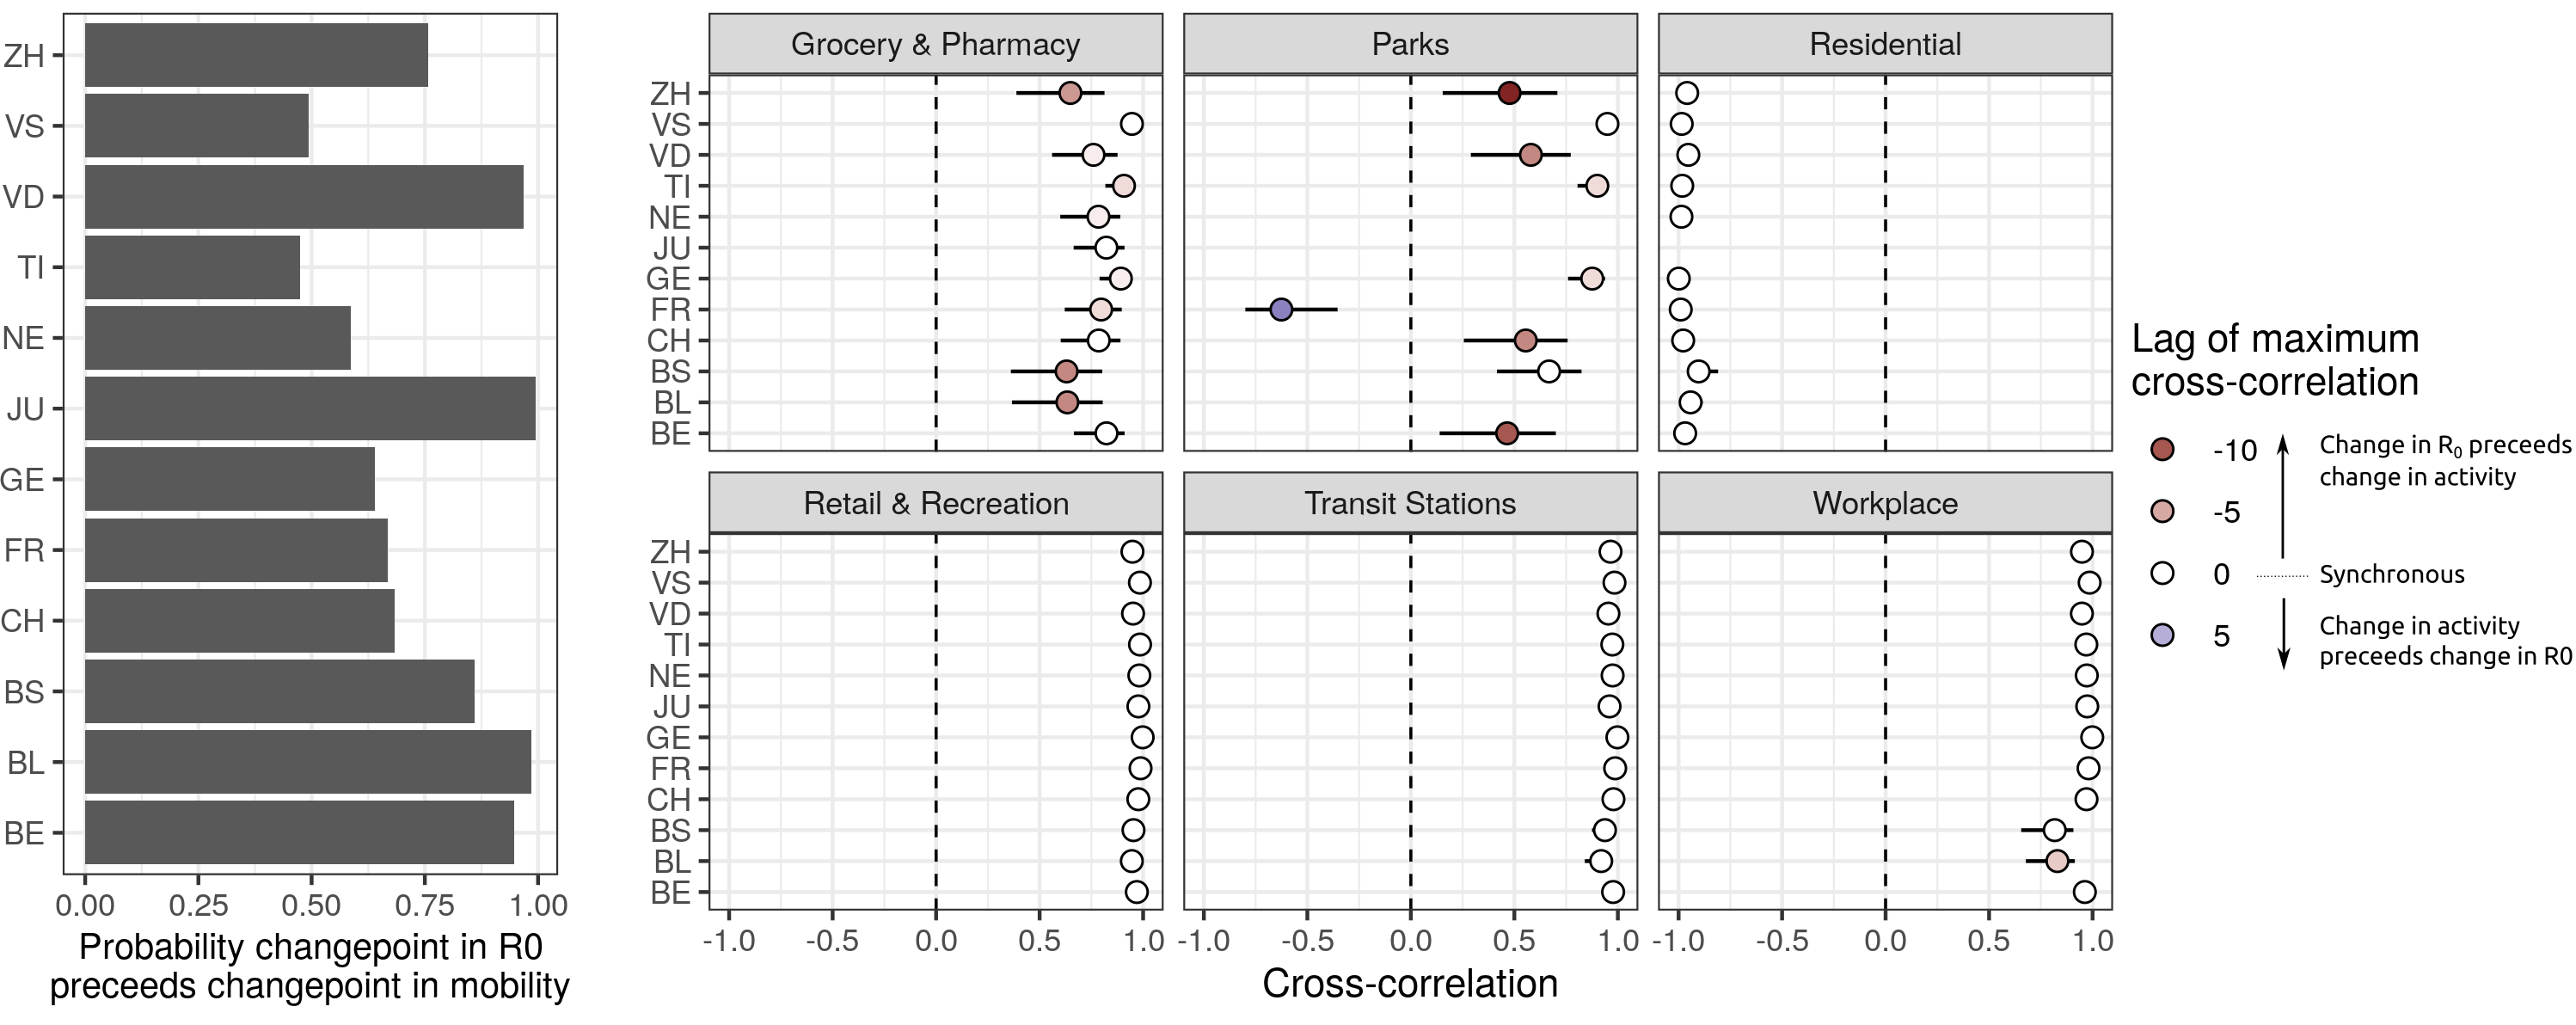
\includegraphics[width=\textwidth]{fig_covid-switzerland-npi/FIGURE_4.png}
  \caption[Timing between changes in $R_0$ and mobility][-2\baselineskip]{Timing between changes in $R_0$ and mobility. Left: probability that the first changepoint in $R_0$ occured before the first changepoint in mobility-related activity. Right: Maximum cross-correlations between time series of changes in $R_0$ and changes in mobility (bars 95\% CI). Lags refer to the delay between changes in mobility-related activity and changes in $R_0$ (positive lag k indicates that current changes in mobility have maximal cross-correlation with changes in $R_0$ $k$ days in the past).}
  \label{fig:covid-ch-timing}
\end{figure*}
In the majority of cases, correlation between mobility and $R_0$ was strongest with no lag between the two. However, changes in mobility to workplaces lagged behind changes in $R_0$ in Basel-Stadt and Basel-Landschaft. Correlations between changes in $R_0$ and grocery and pharmacy mobility were less marked (national level 0.65), with changes in mobility occurring after changes in $R_0$ (negative lags in fig.~\ref{fig:covid-ch-timing}). In most cantons, a strong increase in park mobility after March 25 resulted in a positive correlation with changes in $R_0$, but with negative lags (change in activity after change in $R_0$, fig.~\ref{fig:covid-ch-timing}). 
The linear associations between the level of reduction in mobility and maximum reduction in $R_0$ across cantons was found to be not significant, except for a small effect size for reduced park mobility (regression coefficient of 0.15, 95\% CI 0.02–0.25) (postprint \textsc{si} fig. 8). 

The effective reproduction number $R_{eff}$, a common mesure which is an aggregate measure of transmission capturing aspects of both infectious contacts and of population susceptibility was estimated. Across cantons, $R_{eff}$ was extremely close to $R_0$, indicating that a small fraction of the population is expected to have natural immunity to SARS-CoV-2. 
As of April 24, an estimated 3.9\% (95\% QR 3.6–4.3\%) of the population nationally had been infected, with median estimates ranging from 1.9\% (Bern) to 16\% (Ticino) (fig.~\ref{fig:covid-ch-map}). 
Modelled estimates of the proportion infected of people infected in the canton of Geneva are in agreement with preliminary results from ongoing serological studies, which have estimated the seroprevalence to be 9.7\% (95\% CrI 6.1–13.1\%) in the third week of April\cite[-3\baselineskip]{Stringhini:RepeatedSeroprevalenceAntiSARSCoV2:2020}, compared with modeled estimates of 8.9\% (95\% QR 7.8–10.1\%) after accounting for the time from infection to seroconversion\cite{Wolfel:VirologicalAssessmentHospitalized:2020}(postprint \textsc{si} fig. 7).

\begin{figure}\centering
  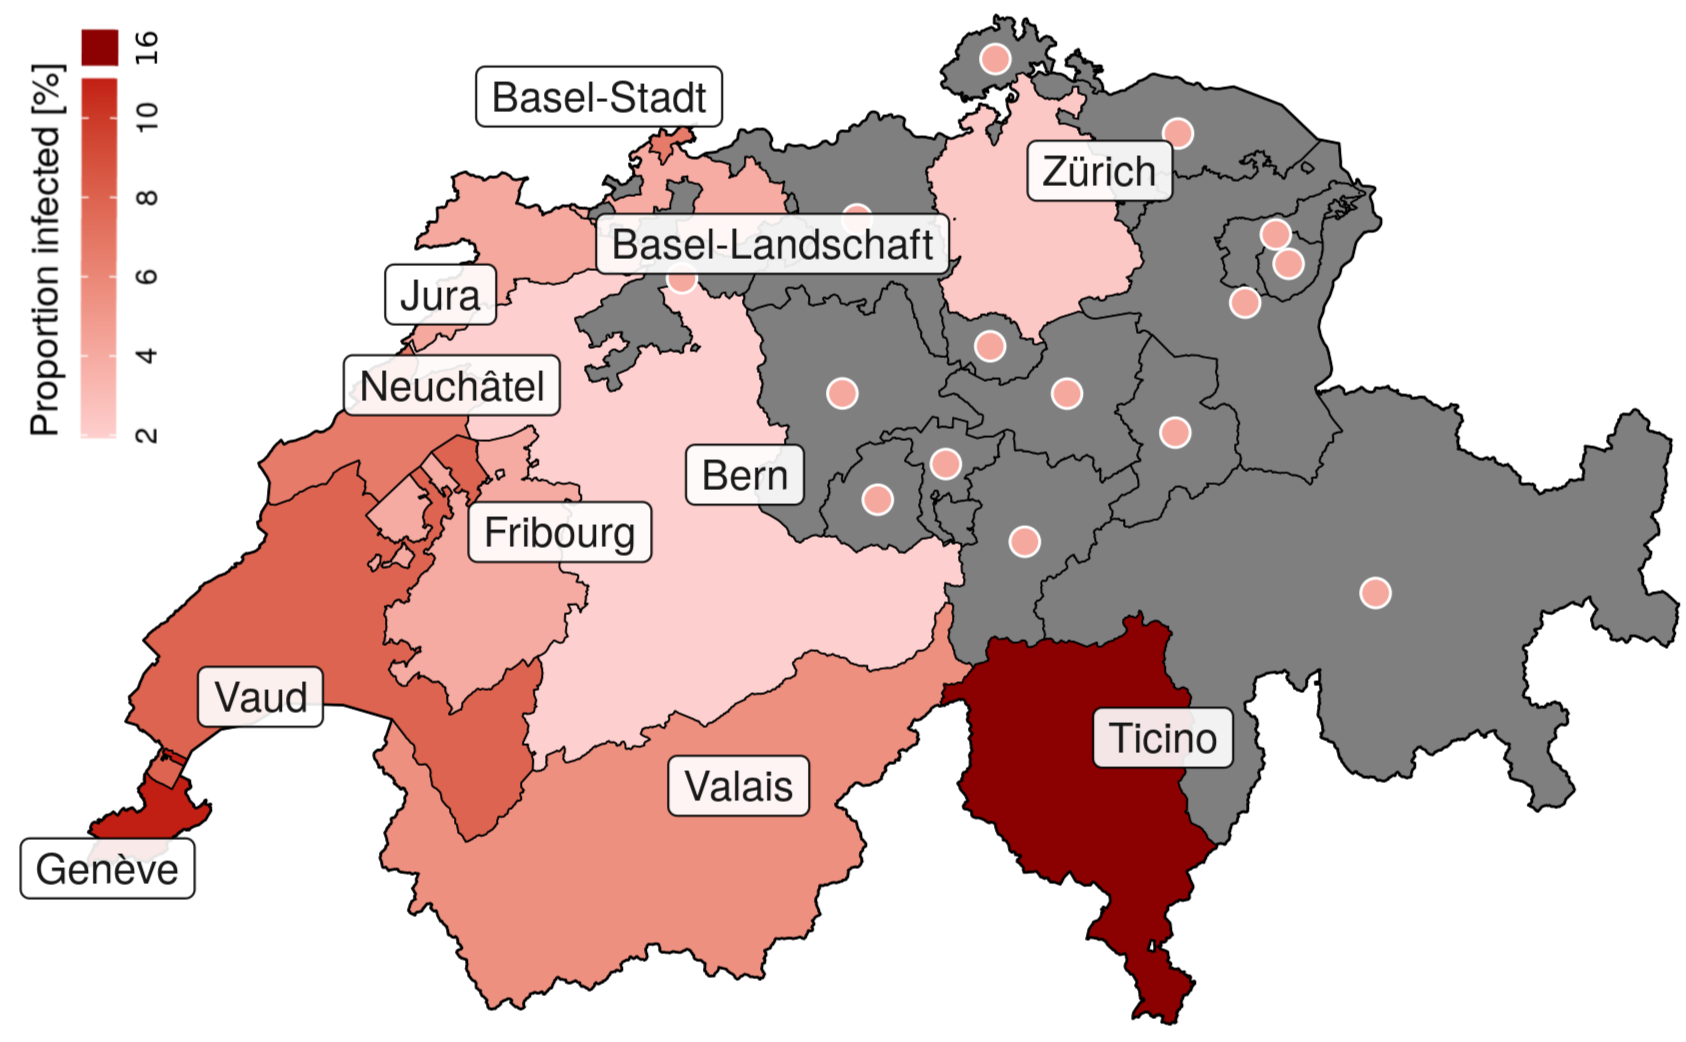
\includegraphics[width=\textwidth]{fig_covid-switzerland-npi/FIGURE_5_mod.png}
  \caption[Modelled proportion of people infected with SARS-CoV-2 in Switzerland][2\baselineskip]{Modelled proportion of people infected with SARS-CoV-2 in Switzerland up to April 24. Estimates were produced for 11 of 26 cantons for which enough data were available (unmodelled cantons are shown in gray with points indicating the national-level estimated incidence proportion of 3\%). Values are reported in the postprint \textsc{si} tab. 6.}
  \label{fig:covid-ch-map}
\end{figure}

\section{Discussion}
Our results suggest a strong reduction of $R_0$ across Switzerland since the start of the epidemic. The reduction in $R_0$ started around March 7, thus about 1 week before the implementation of lockdown-type NPIs. Analysis of activity-related mobility data also showed strong support for changes in mobility starting prior to the implementation of most NPIs. Estimated reductions of viral transmission were strongly correlated and mostly synchronous with observed changes in mobility patterns, although the initiation of changes in transmission preceded measurable changes in activity-related mobility. 

The methods used to infer the time series of $R_0$ do not rely on assumptions on the shape of how it changed in time, nor on the dates at which change started. Alternative methods that rely on fixed dates (such as that of the Imperial College \textsc{covid}-19 Response Team\cite[-6\baselineskip]{Flaxman:Report13Estimating:2020}) might be biased as changes in transmission are not synchronous with policy changes. Distribution based methods such as provided by R package EpiEstim\cite[-4\baselineskip]{Wallinga:DifferentEpidemicCurves:2004,Cori:NewFrameworkSoftware:2013} are flexible but subject to bias when misused\cite{Lipsitch:CommentPanLiu:2020}. In addition, the present approach enables the estimation of $R_0$, which is a direct quantification of transmission potential, as opposed to the effective reproduction number $R_{eff}$, which also accounts for the effect of susceptible depletion as done in the above-mentioned statistical approaches. This enabled us to estimate the proportion of reduction in transmission attribuable to behavioural changes, which is therefore more suited to study the impact of NPIs. Aside from these methodological differences, the present estimates are in line with other estimates in Switzerland: Althaus et al.\cite{Althaus:RealtimeModelingProjections:2020} estimated a reduction of 89 \% (83–94\%) from a baseline of 2.78 (2.51–3.11), Scire et al.\cite{Scire:ReproductiveNumberCOVID19:2020} estimated a reduction of 76 \% (70–82\%) from a baseline of 1.88 (1.80–1.98) and Imperial College estimated a reduction of 60\% (50–80\%) from a baseline of 3.5 (2.8–4.3)\cite{Flaxman:Report13Estimating:2020}. 

The presented results provide strong support for a reduction of transmission starting about 1 week prior to school closure, the first national-level NPI targeting daily activities, which was ordered on March 13. Moreover, initiation of transmission reduction was found to precede changes in mobility patterns as detectable from the Google dataset. A possible explanation for this initial decrease in transmission could be linked to the strong increase in public interest in \textsc{covid}-19 in February as measured by Google searches for \textsc{covid}-19-related keywords (fig.~\ref{fig:googlemob}).
\begin{marginfigure}[1\baselineskip]
%\centering
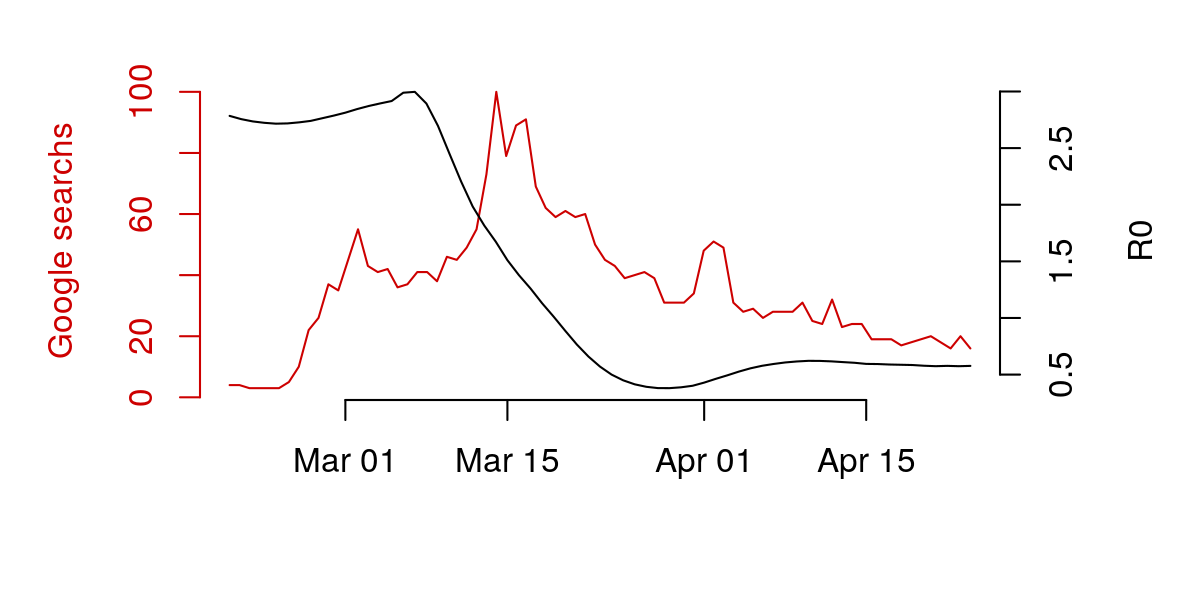
\includegraphics{fig_covid-switzerland-npi/fig_supp/google_trends.png}
\margincaption[Google trends for \textsc{covid}-19 and changes in R$_0$ in Switzerland]{\footnotesize Google trends for \textsc{covid}-19 and changes in R$_0$ in Switzerland. Trends corresponds to amount of searches for the keyword "coronavirus" (red line) between February 15 and April 30 and are given as a percent of the maximum number of searches in the period, time evolution of R$_0$.}\label{fig:googlemob}
\end{marginfigure}
 In fact, a second sharp rise in Google searches is estimated to have started on March 7 (95\% CrI March 3–9), which overlaps with the estimated start of national level decrease in $R_0$ on March 7 (probability that changepoints coincide 0.76). The Federal Office for Public Health issued an information campaign on \textsc{covid}-19 on February 28, which was updated on March 2 to stress basic hygiene rules\cite{OFSP:NouvellesReglesHygiene:2020}. This may have resulted in voluntary social distancing as well as increased hygiene early on without noticeable changes in mobility patterns. This type of proactive change in behaviour would be in line with early changes in mobility patterns, which were estimated to precede school closures and subsequent measures. The present results suggest that the value of $R_0$ was likely already below one on March 20, when the federal government banned gatherings of more than five people and recommended voluntary home isolation for the whole population. This result should however be taken within context, as the announcement was anticipated on social networks earlier that week, and so was probably already impacting social distancing behaviour. 
Therefore caution is recommend in any causal interpretation of these results on the role of this last NPI on driving $R_0$ below one.

Despite the strong association between the changes in mobility and reductions in $R_0$ within each canton, the lack of cross-cantonal associations between the level of reduction in mobility types and the level of reduction in $R_0$ suggests context-specific pathways between \textsc{covid}-19 transmission and mobility intensity. This warrants caution in attempting to apply general relations between mobility and transmission reduction. Investigation of general associations will require more in-depth studies controlling for other factors such as population density, economic activities and social mixing patterns, and inter-cantonal mobility patterns, in addition to incorporation of potential environmental drivers of transmission such as temperature and relative humidity\cite{Neher:PotentialImpactSeasonal:2020, Kissler:ProjectingTransmissionDynamics:2020}. 
  
  Several limitations to this work are noted. First, due to the relatively recent introduction of SARS-CoV-2 in Switzerland compared with the length of hospital and ICU stays, the time distribution of hospital in- and out-patients is biased towards shorter duration (see \textsc{Appendix}), which is addressed by accounting with right-censoring using survival models. In addition, because of the limited data available in some places, it was only possible to fit the model for 11 of the 26 cantons. Modelling results presented in this work are subject to hypothesis on yet uncertain parameters of \textsc{covid}-19, including the infection fatality rate and the proportion of severe infections requiring hospitalisation. An important uncertainty is the fraction of asymptomatic infections and their relative contribution to disease transmission. It is assumed that all infected individuals contribute equally to transmission, which means the estimation of the proportion of people infected would under-estimate true cumulative incidence if there were a large fraction of asymptomatic infections with a relatively low contribution to transmission. Evidence from South Korea, however, suggests that only a small fraction (2\%) of confirmed \textsc{covid}-19 infections are totally asymptomatic, and none of the household members of these asymptomatic carriers were infected\cite[-4\baselineskip]{Park:EarlyReleaseCoronavirus:2020}. Moreover, model results are in agreement with preliminary results from ongoing serological studies in Switzerland\cite[-2\baselineskip]{Stringhini:RepeatedSeroprevalenceAntiSARSCoV2:2020}.  The presented estimates of time-varying basic reproduction numbers assume that the generation interval for \textsc{covid}-19 in Switzerland remained unchanged, thus potentially ignoring the joint role of $R_0$, the infectious period and contact rates in determining the disease’s intrinsic growth rate\cite{Yan:SeparateRolesLatent:2008}. If the generation interval increased with the reduction of social contact then these estimates are conservative overestimates of the “true” value of $R_0$, which is encouraging from a public health perspective. Inferred disease dynamics and estimated time-varying $R_0$ also depend on the values of the incubation period, which is set to the estimates currently available in the literature. 
  In the present modelling framework, the initial conditions were estimated along with changes in $R_0$, which could, however, be influenced by the role of imported cases in driving disease dynamics, especially in cantons bordering regions with strong \textsc{covid}-19 transmission in early February (Eastern France for Basel-Stadt and Basel-Landschaft and Northern Italy for Ticino). 
  Since importations were not modeled, this could yield an overestimation of the initial value of $R_0$, which warrants caution in interpreting specific values of $R_0$ in these cantons. This potential overestimation would, however, not affect the strong inferred reduction in $R_0$. Another limitation of this study is that it was not possible to disentangle the individual contribution of each NPI on $R_0$ in this analysis owing to the early onset of changes in $R_0$ and in mobility patterns, as well as the very close spacing between the different types of NPI. This information would, however, be extremely valuable in supporting decisions on NPI strategies against \textsc{covid}-19. Efforts to constitute a global database of NPIs will provide the opportunity to extend this type of analysis to other settings and produce evidence for the effect of different types of NPIs\cite{HITCOVIDTeam:HealthInterventionsTracking:2020}. 
  
  As the Swiss government plans to gradually lift restrictions, close monitoring of changes in $R_0$ is critical, given that the reductions in transmission appear to be almost entirely driven by changes in behaviour, not through herd immunity. Near real-time estimates of $R_0$ may serve as a critical tool for public health and political decision makers in the months to come, and efforts should be made to refine models like ours using new data, including those from population-based serological studies, mobility data and more detailed individual-level data on \textsc{covid}-19 cases across the spectrum of severity.\marginnote[-4\baselineskip]{While relying on hospitalization and death allowed for an early robust identification of the basic reproduction number, it would be necessary to add a reporting process and case data to update this estimate through 2020-2021. Methods based on observed data are easier to maintain, and reliable continuous updates of the reproduction number in Switzerland available on the Swiss National \textsc{covid}-19 Task Force website \url{sciencetaskforce.ch/en/current-situation/}. It is provided by the ETHZ, with method described in \fullcite{Huisman:EstimationWorldwideMonitoring:2021}. The modeled incidence from the present Chapter has been later used as "truth" to compare waste-water data with reported cases, see: \fullcite{Fernandez-Cassi:WastewaterMonitoringOutperforms:2021}.}





%%
% The back matter contains appendices, bibliographies, indices, glossaries, etc.

\backmatter

%\bibliography{sample-handout}
%\bibliographystyle{plainnat}
%\printbibliography

\printindex

\end{document}

